\documentclass{book}
\usepackage[english]{babel}     
\usepackage[utf8]{inputenc}     % accent symbols
\usepackage[T1]{fontenc}
\usepackage{lmodern}
\usepackage{microtype}
\usepackage{natbib}
\usepackage{tocbibind}          
\usepackage{amsmath}            % math symbols
\usepackage{amsthm}             % math symbols
\usepackage[colorlinks=true,linkcolor=red]{hyperref} % hyper link

% for code
\usepackage{listings}
\usepackage{color,xcolor}
\definecolor{mygreen}{rgb}{0,0.6,0}
\definecolor{mygray}{rgb}{0.9,0.9,0.9}
\definecolor{mymauve}{rgb}{0.58,0,0.82}
\lstset{
backgroundcolor=\color{mygray},
numbers=left,                    
columns=fullflexible,
breaklines=true,      
captionpos=b,         
tabsize=4,            
commentstyle=\color{mygreen}, 
escapeinside={\%*}{*)},       
keywordstyle=\color{blue},    
% stringstyle=\color{mymauve}\monaco,
frame=single,                        
rulesepcolor=\color{red!20!green!20!blue!20},
% identifierstyle=\color{red},
%% language=c++,
basicstyle=\tiny
}

\usepackage{indentfirst}
\setlength{\parindent}{2em}
\usepackage[onehalfspacing]{setspace}
% graph
\usepackage{pdfpages}
\usepackage{graphicx}
% box
\usepackage{booktabs}
\usepackage{tcolorbox}

%% user defined command
\newcommand{\keyword}[1]{\textbf{#1}}
\newcommand{\keywords}[1]{\textbf{#1}}
\newcommand{\lcmd}[1]{\texttt{#1}}
\newcommand{\head}[1]{\textnormal{\textbf{#1}}}
\newcommand{\itwords}[1]{\textit{#1}}

\usepackage{float}
% all symbols
\usepackage{tipa}
\usepackage{tipx}

\usepackage{datetime}
% \usepackage{movie15}


% variable
% TODO
\newcommand{\pdfauthor}{Mike Chyson (Li Mingming)}
\newcommand{\pdftitle}{Principles of Economics}
\newcommand{\pdfsubject}{Principles of Economics}
\newcommand{\pdfkeywords}{Principles of Economics}
\newcommand{\bookname}{Principles of Economics}
\newcommand{\bookoneword}{Citation and interpreation of principles of economics}
\newcommand{\timeandcompany}{Dec, 5, 2020}

\usepackage{bm}
\usepackage{amsfonts}
\hypersetup{
  pdfauthor={\pdfauthor},   
  pdftitle={\pdftitle},     
  pdfsubject={\pdfsubject}, 
  pdfkeywords={\pdfkeywords}
}
% \includeonly{}
\begin{document}
\frontmatter
\begin{titlepage}
  \raggedleft
      {\Large 作者\\ 李明明\\[1in] }
  % {\large 关于\\}
  {\Huge\scshape 法语学习\\[.2in]}
  {\large 从零学习法语的笔记整理 \\}
  \vfill
  {\itshape \today{}}
\end{titlepage}


\chapter*{Dedication}

读《经济学原理》的笔记。


\mainmatter
\tableofcontents


% \listoftables
% \listoffigures


\chapter{Introduction}

\section{Creating and running Pyton programs}

Be default, Python files are assumed to use the UTF-8 character encoding.
Python files normally have an extension of \verb|.py|.
Python GUI (Graphical User Interface) programs usually have an extension of \verb|.pyw|.



\begin{lstlisting}
  #!/usr/bin/env python3

  print("Hello", "world")
\end{lstlisting}



The first line is a comment.
In Python,comments begin with a \verb|#| and continue to the end of the line.
The second line is blank.
Python ignores blank lines, but they are often useful to humans to break up large blocks of code to make them easier to read.
The third line is Python code.


Each statement encountered in a \verb|.py| file is executed in turn, starting with the first one and progressing line by line.
Python programs are executed by the Python interpreter, and normally this is done inside a console window.



On Unix, when a program is invoked in the console, the file's first two bytes are read.
If these bytes are the ASCII chracters \verb|#!|, the shell assume that the file is to be executed by an interpreter and that the file's first line specifies which interpreter to use.
This line is called the \keyword{shebang} (shell execute) line, and if the present must be the first line in the file.



The shebang line is commonly written in one of two forms, either:
\begin{lstlisting}
#!/usr/bin/python3
\end{lstlisting}

or

\begin{lstlisting}
#!/usr/bin/env python3
\end{lstlisting}


If written using the first form, the specified interpreter is used.
If written using the second form, the first \verb|python3| interpreter found in the shell's current environment is used.
The second form is more versatile because it allows for the possibility that the Python 3 interpreter is ont located in \verb|/usr/bin|



\section{Python's "Beautiful Heart"}


\subsection{Data types}


One fundamental thing that any programming language must be able to do is represent items of data.

The size of Python's integers is limited only by machine memory, not by a fixed number of bytes.
Strings can be delimited by double or single quotes, as long as the same kind are used at both ends.


\begin{lstlisting}
210624583337114373395836055367340864637790190801098222508621955072
0
"hello"
'world'
\end{lstlisting}


Python uses square brackets ([]) to access an item from a sequence such as a string.

\begin{lstlisting}
'Hello World'[4]
\end{lstlisting}


In Python, both \verb|str| and the basic numeric types such as \verb|int| are \keyword{immutable}.
At first this appears to be a rather strange limitation, but Python's syntax means that this is a nonissue in practice.
The only reason for mentioning it is that although we can use square brackets to retrieve the character at a given index position in a string, we cannot use them to set a new character.



To convert a data item from one type to another we can use the syntax \verb|datatype(item)|.
\begin{lstlisting}
int("45")
str(123)
\end{lstlisting}



\subsection{Object references}

Once we have some data types, the next thing we need are variables in which to store them.
Python doesn't have variables as such, but instead has \keyword{object references}.
When it comes to immutable objects like \verb|int|s and \verb|str|s, there is no discernable difference between a variable and an object reference.
As for mutable objects, there is a difference, but it rarely matters in practice.



\begin{lstlisting}

x = "blue"
y = "green"
z = x
\end{lstlisting}


The syntax is simply \verb|object_reference = value|.
The \verb|=| operator is not the same as the variable assignment operater in some other languages.
The \verb|=| operater binds an object reference to an object in memory.
If the object reference already exists, it is simply re-bound to refer to the object on the right of the \verb|=| operator;
if the object reference does not exist it is created by the \verb|=| operator.


Python uses \keyword{dynamic typing}, which means that an object reference can be rebound to refer to a different object at any time.
Languages that use strong typing (such as C++ and Java) allow only those operations that are defined for the data types involved to be performed.
Python also applies this constraint, but it isn’t called strong typing in Python’s case because the valid operations can change --- for example, if an object reference is re-bound to an object of a different data type.

\begin{lstlisting}

route = 123
print(route, type(route))

route = "North"
print(route, type(route))
\end{lstlisting}



The \verb|type()| function returns the data type (also known as the ``class'') of the data item it is given --- this function can be very useful for testing and debugging, but would not normally appear in production code.


\subsection{Collection data types}

To hold entire collections of data items, Python provides several collection data types that can hold items.
Python tuples and lists can be used to hold any number of data items of any data types.
Tuples are imuutable while lists are mutable.


Tuples are created using commas (,), as these examples show:
\begin{lstlisting}

>>> "hello", "world", "mike", "chyson"
("hello", "world", "mike", "chyson")
>>> "one",
("one",)
\end{lstlisting}


When Python ouptuts a tuple it encloses it in parentheses.
An empty tuple is created by using empty parentheses, ().
The comma is also used to separate arguments in function calls, so if we want to pass a tuple literal as an argument we must enclose it in parentheses to avoid confusion.


\begin{lstlisting}

[1,2,3]
[]
\end{lstlisting}

One way to create a list is to use square brackets ([]).
An empty list is create by using empty brackets, [].


Under the hood, lists and tuples don't store data items at all, but rather object references.
When lists and tuples are created (and when items are inserted in the case of lists), they take copies of the object references they are given.
In the case of literal items such as integers or strings, an object of the appropriate data type is created in memory and suitably initialized, and then an object reference referring to the object is created, and it is this object reference that is put in the list or tuple.



In precedural programming we can function and often pass in data items as arguments.
\begin{lstlisting}

>>> len(("one",))
1
>>> len([1, 2, "hell", 3])
4
\end{lstlisting}



All Python data items are \keyword{objects} (also called \keyword{instances}) of a particular data type (also called a class).



\begin{lstlisting}

>>> x = ["zebra", 49, -879, "aardvark", 200]
>>> x.append("more")
>>> x
['zebra', 49, -879, 'aardvark', 200, 'more']

>>> list.append(x, "extra")
>>> x
['zebra', 49, -879, 'aardvark', 200, 'more', 'extra']
\end{lstlisting}


Python has conventional functions called like this \verb|function_name(arguments)|;
and methods which are called like this \verb|ojbect_name.method_name(arguments)|.

The dot (``access attribute'') operator is used to access an object's attributes.

\section{Logical operations}

Python provides four sets of logical operations.


\subsection{The identity operator}

The \verb|is| operator is a binary operator that returns \verb|True| if its left-hand object reference is referencing to the same object as its right-hand object reference.


\begin{lstlisting}
>>> a = ["Retention", 3, None]
>>> b = ["Retention", 3, None]
>>> a is b
False
>>> b = a
>>> a is b
True
\end{lstlisting}



One benefit of identity comparisons is that they are very fast.
This is because the objects referred to do not have to be examined themselves.
The is operator needs to compare only the memory addresses of the objects --- the same address means the same object.



The most common use case for \verb|is| is to compare a data item with the built-in null object, \verb|None|.



The purpose of the identity operator is to see whether two object references refer to the same object, or to see whether an object is \verb|None|.
If we want to compare object values we should use a comparison operator instead.

\subsection{Comparison operators}

Python provides the standard set of binary comparison operators:

\begin{itemize}
\item <
\item <=
\item ==
\item !=
\item >=
\item >
\end{itemize}

These operators compare object values, that is, objects that the object references used in the comparison refer to.


In some cases, comparing the identity of two strings or numbers will return \verb|True|, even if each has been assigned separately.
This is because some implementations of Python will reuse the same object (since the value is the same and is immutable) for the sake of efficiency.
The moral of this is to use \verb|==| and \verb|!=| when comparing \keyword{values}, and to use \verb|is| and \verb|is not| only when comparing with \verb|None| or when we really do want to see if two object references, rather than their values, are the same.



One particularly nice feature of Python’s comparison operators is that they can be chained.
For example:
\begin{lstlisting}

>>> a = 9
>>> 0 <= a <= 10
True
\end{lstlisting}



This is a nicer way of testing that a given data item is in range than having to do two separate comparisons joined by logical \verb|and|.
It also has the additional virtue of evaluating the data item only once (since it appears once only in the expression), something that could make a difference if computing the data item's value is expensive, or if accessing the data item causes side effects.


\subsection{The membership operator}

For data types that are sequences or collections such as strings, lists, and tuples, we can test for membership using the \verb|in| operator, and for nonmembership using the \verb|not in| operator. For example:
\begin{lstlisting}

>>> p = (4, "frog", 9, -33, 9, 2)
>>> 2 in p
True
>>> "dog" not in p
True
\end{lstlisting}



For lists and tuples, the \verb|in| operator uses a linear search which can be slow for very large collections (tens of thousands of items or more).
On the other hand, \verb|in| is very fast when used on a dictionary or a set.



\subsection{Logical operators}

Python provides 3 logical operators:
\begin{itemize}
\item and
\item or
\item not
\end{itemize}


Both \verb|and| and \verb|or| use short-circuit logic and return the operand that determined the result -- they do not return a Boolean (unleass they actually have Boolean operands).


\begin{lstlisting}

>>> five = 5
>>> two = 2
>>> zero = 0
>>> five and two
2
>>> two and five
5
>>> five and zero
0
\end{lstlisting}



If the expression occurs in a Boolean context, the result is evaluated as a Boolean, so the preceding expressions would come out as \verb|True|, \verb|True|, and \verb|False|.

\begin{lstlisting}

>>> nought = 0
>>> five or two
5
>>> two or five
2
>>> zero or five
5
>>> zero or nought
0
\end{lstlisting}



The \verb|or| operator is similar; here the results in a Boolean context would be \verb|True|, \verb|True|, \verb|True|, and \verb|False|.


The \verb|not| unary operator evaluates its argument in a Boolean context and always returns a Boolean result.


\section{Control flow statements}

A Boolean expression is anything that can be evaluated to produce a Boolean value (\verb|True| or \verb|False|).
In Python, such an expression evaluate to \verb|False| if it is the predefined constant \verb|False|, the special object \verb|None|, an empty sequence or collection, or a numeric data item of value 0; anything else is considered to be \verb|True|.


In Python-speak a block of code, that is, a sequence of one or more statements, is called a \keyword{suite}.
Because some of Python's syntax requires that a suite be present, Python provides the keyword \verb|pass| which is a statement that does nothing and that can be used where a suite is required but where no precessing is necessary.



\subsection{The if statement}

\begin{tcolorbox}
\begin{verbatim}
if boolean_expression1:
    suite1
elif boolean_expression2:
    suite2
...
elif boolean_expressionN:
    suiteN
else:
    else_suite
\end{verbatim}
\end{tcolorbox}


Colons are used with \verb|else|, \verb|elif|, and essentially in any other place where a suite is to follow.
Unlike most other programming languages, Python uses indentation to signify its block structure.


\subsection{The while statement}

\begin{tcolorbox}
\begin{verbatim}
while boolean_expression:
    suite
\end{verbatim}
\end{tcolorbox}


\subsection{The for ... in statement}

\begin{tcolorbox}
\begin{verbatim}
for variable in iterable:
    suite
\end{verbatim}
\end{tcolorbox}


The \verb|variable| is set to refer to each object in the \verb|iterable| in turn.


\subsection{Basic exception handling}

An exception is an object like any other Python object, and when converted to a string, the exception produces a message text.
A simple form of the syntax for exception handlers is this:
\begin{tcolorbox}
\begin{verbatim}
try:
    try_suite
except exceptions1 as variable1:
    exception_suite1
...
except exceptionN as variableN:
    exception_suiteN
\end{verbatim}
\end{tcolorbox}

The \verb|as variable| part is optional.


\begin{verbatim}
s = input("enter an integer: ")
try:
    i = int(s)
    print("valid integer entered:", i)
except ValueError as err:
    print(err)
\end{verbatim}


\section{Arithmetic operators}

Four basic mathematical operations:
\begin{itemize}
\item +
\item -
\item *
\item /
\end{itemize}

In addition, many Python data types can be used with augmented assignment operators such as:
\begin{itemize}
\item +=
\item -=
\item *=
\item /=
\end{itemize}


The \verb|+|, \verb|-|, and \verb|*| operators all behave as expected when both of their operands are integers.
Where Python differs from the crowd is when it comes to division:
\begin{lstlisting}

>>> 12/3
4.0
\end{lstlisting}


The division operator produces a floating-point value, not a integer.
If we nned an integer result, we can always convert using \verb|int()| or use the truncating devision operator \verb|//|.


\begin{lstlisting}

>>> a = 5
>>> a
5
>>> a += 8
>>> a
13
\end{lstlisting}


Comparing to C-like languages, there are two important subtleties, one Python-specific and one to do with augmented operators in any language.


The first point to remember is that the \verb|int| data type is immutable.
So, what actually happens behind the scenes when an augmented assignment operator is used on an immutable object is that the operation is performed, and an object holding the result is created; and then the target object reference is re-bound to refer to the result object rather than the object it referred to before.


The second subtlety is that \verb|a operator= b| is not quite the same  as  \verb|a = a operator b|.
The augmented version looks \verb|a|'s value only once, so it is potentially faster.


\begin{lstlisting}

>>> name = 'mike'
>>> name + 'chyson'
'mikechyson'
>>> name += ' chyson'
>>> name
'mike chyson'
>>> a = [1, 2, 3]

>>> a + [4]
[1, 2, 3, 4]
>>> a += [4]
>>> a
[1, 2, 3, 4]
\end{lstlisting}


Python overloads the \verb|+| and \verb|+=| operators for both strings and lists, the former mearning concatenation and the latter meaning append for strings and extend (append another list) for lists.


\section{Input/output}

Rediction:
\begin{itemize}
\item > (output)
\item < (input)
\end{itemize}


Function:
\begin{itemize}
\item input()
\item print()
\end{itemize}



\section{Creating and calling functions}

\begin{tcolorbox}
\begin{verbatim}
def function_name(arguments):
    suite
\end{verbatim}
\end{tcolorbox}

The \verb|arguments| are optional and multiple arguments must be comma-separated.
Every Python function has a return value; this defaults to \verb|None| unless we return from the function using the syntax \verb|return value|, in which case \verb|value| is returned.



\verb|def| is a statement that works in a similar way to the assignment operator.
When \verb|def| is executed a function object is created and an object reference with the specified name is created and set to refer to the function object.
Since functions are objects, they can be stored in collection data types and passed as arguments to other functions.



Although creating our own functions can be very satisfying, in many cases it is not necessary.
This is because Python has a lot of functions built in, and a great many more functions in the modules in its standard library, so what we want may well already be available.


A Python module is just a \verb|.py| file that contains Python code.
To access the functionality in a module we must import is.
For example:
\begin{lstlisting}

import sys
\end{lstlisting}



To import a module we use the \verb|import| statement followed by the name of the \verb|.py| file, but omitting the extension.
Once a module has been imported, we can access any functions, classes, or variables that it contains. For example:

\begin{lstlisting}

print(sys.argv)
\end{lstlisting}




In general, the syntax for using a function from a module is \\
$\mathtt{module\_name.function\_name(arguments)}$.
It makes use of the dot (“access attribute”) operator.




It is conventional to put all the import statements at the beginning of \verb|.py| files, after the shebang line, and after the module’s documentation.
We recommend importing standard library modules first, then third-party library modules, and finally your own modules.


\begin{tcolorbox}
python template:
\begin{verbatim}
--------------------------------
|shebang part                  |
|(like /usr/bin/env python3)   |
|                              |
|------------------------------|
|                              |
|documentation part            |
|                              |
|------------------------------|
|                              |
|import part                   |
|  ----------------------------|
|  | import standard library   |
|  | import third-party library|
|  | import own library        |
|  ----------------------------|
|------------------------------|
|                              |
|code                          |
|                              |
--------------------------------
\end{verbatim}
\end{tcolorbox}

\chapter{Data types}

\section{Identifiers and keywords}

The name we give to our object references are called \keyword{identifiers} or just plain \keyword{names}.



A valid Python identifier is a \keyword{nonempty} sequence of characters of any length that consists of a ``start character'' and zero or more ``continuation characters''.
Such an identifier must obey a couple of rules and ought to follow certain conventions.


Rules:
\begin{itemize}
\item The start character can be anything that Unicode considers to be a letter.
\item Each continuation character can be any character that is permitted as a start character, or any nonwhitespace character.
\item No identifier can have the same name as one of Python's keywords.
\end{itemize}


Python has a built-in function called \verb|dir()| that returns a list of object's attributes.


Conventions:
\begin{itemize}
\item Don't use the name of any of Python's predefined identifiers for your own identifiers.
\item Names that begin and end with two underscores should not be used.
\end{itemize}


\section{Integral types}

Python provides two built-in integral types, \verb|int| and \verb|bool|.
Both integers and Boolean are imuutable.
When used in Boolean expressions, 0 and \verb|False| are \verb|False| and any other integer and \verb|True| are \verb|True|.
When used in numerical expressions \verb|True| evaluates to 1 and \verb|False| to 0.



\subsection{Integers}

Integer literals are written using base 10 by default, but other number bases can be used.

\begin{lstlisting}

>>> 14600926                      # decimal
14600926
>>> 0b110111101100101011011110    # binary
14600926                          
>>> 0o67545336                    # octal
14600926
>>> 0xDECADE                      # hexadecimal
14600926
\end{lstlisting}



Binary numbers are written with a leading \verb|0b|,
octal numbers with a leading \verb|0o|, and
hexadecimal numbers with a leading \verb|0x|.
Uppercase letters can also be used.



All the usual mathematical functions and operators can be used with integers.
Some of the functionality is provided by functions and other functionality is provided by \verb|int| operators.


Provided by operators:
\begin{description}
\item[x + y] 
\item[x - y]
\item[x * y] 
\item[x / y] Divdes $x$ by $y$; always produces a \verb|float| (or a \verb|complex| if $x$ or $y$ is \verb|complex|)
\item[x // y] Divdes $x$ by $y$; truncates any fractional part so always produces an \verb|int| result
\item[x \% y]   
\item[x ** y] Same to $x^y$
\item[-x] Negates x;
\item[+x] Does nothing; is sometimes used to clarify code
\item[x | y] Bitwise \verb|OR| 
\item[x \^{} y] Bitwise \verb|XOR|
\item[x \&{} y|] Bitwise \verb|AND|
\item[i $>>$ j] Shifts \verb|i| left by \verb|j|; like \verb|i * (2 ** j)| without overflow checking
\item[i $<<$ j] Shifts \verb|i| right by \verb|j|; like \verb|i // (2 ** j)| without overflow checking
\item[\~{}i]  Inverts \verb|i|'s bits
\end{description}

Provided by functions:
\begin{description}
\item[abs(x)] Return the absolute value of $x$
\item[divmod(x, y)] Return the quotient and remaninder of dividing $x$ by $y$ as a tuple of two \verb|int|s
\item[pow(x, y)] Same to $x^y$
\item[pow(x, y, z)] A faster alternative to $(x ** y) \% z$
\item[round(x, n)] Return $x$ rounded to $n$ integral digits if $n$ is a negative \verb|int| or return $x$ rounded to $n$ decimal places if $n$ is a positive \verb|int|; the returned value has the same type as x;
\item[bin(i)] Return the binary representation of \verb|int i| as a string
\item[hex(i)] 
\item[int(x)] Convert object $x$ to an integer
\item[int(s, base)] Convert \verb|str s| to an integer. \verb|base| should be an integer between 2 and 36 inclusive.
\item[oct(i)] 
\end{description}



All the binary numeric operators (+, -, /, //, \%, and **) have augmented assignment versions (+=, -=, /=, //=, \%=, and **=) where \verb|x op= y| is logically equivalent to \verb|x = x op y| in the normal case when reading x’s value has no side effects.

All the binary bitwise operators (|, \^{}, \&{}, $<<$, and $>>$) have augmented assignment versions (|=, \^{}=, \&{}=, $<<=$, and $>>=$) where \verb|i op= j| is logically equivalent to \verb|i = i op j| in the normal case when reading \verb|i|’s value has no side effects.


\begin{tcolorbox}
When an object is created using its data types there are 3 possible use cases:
\begin{enumerate}
\item When a data type is called with no arguments an object with a default value is created.
\item When the data type is called with a sinle argument, if an argument of the same type is given, a new object which is a shallow copy of the original object is created. If argument of a different type is given, a conversion is attempted.
\item If two or more arguments are given --- not all types support this, and for those that do the argument types and their meanings vary.
\end{enumerate}
\end{tcolorbox}


\subsection{Booleans}

There are two built-in Boolean objects: \verb|True| and \verb|False|.

\section{Floating-point types}

Python provides three kinds of floating-point values:
\begin{itemize}
\item the built-in \verb|float|
\item the built-in \verb|complex|
\item the \verb|decimal.Decimal| type from the standard library
\end{itemize}
All three are immutable.


\verb|decimal.Decimal| perform calculations that are accurate to the level of precision we specify (by default, to 28 decimal places) and can represent periodic numbers like 0.1 exactly; but processing is a lot slower than with \verb|float|s.
Because of their accuracy, \verb|decimal.Decimal| numbers are suitable for financial calculations.



\subsection{Floating-point numbers}

\begin{tcolorbox}
  \begin{lstlisting}

import sys

# the samllest difference that the machine can distinguish 
# between two floating-point numbers
sys.float_info.epsilon 

help(sys.float_info)
  \end{lstlisting}
\end{tcolorbox}

The \verb|math| module provides many functions that operate on \verb|float|s.
The \verb|math| module is very dependent on the underlying math library that Python was compiled against.
This means that some error conditions and boundary cases may behave differently on different platforms.


\begin{description}
\item[math.copysign(x, y)] Returns \verb|x| with \verb|y|'s sign
\item[math.e] 
\item[math.pi] 
\item[math.exp(x)] 
\item[math.factorial(x)] Returns $x!$
\item[math.floor(x)] 
\item[math.ceil(x)] 
\item[math.hypot(x, y)] Returns $\sqrt(x^2 + y^2)$
\item[math.isinf(x)] Returns \verb|True| if \verb|float x| is $\pm \mathrm{inf}(\pm \infty)$
\item[math.isnan(x)] Returns \verb|True| if \verb|float x| is nan (``not a number'')
\item[math.log(x, b)] Returns $\log_bx$
\item[math.log10(x)] Returns $\log_{10}x$
\item[math.sqrt(x)] 
\end{description}




\subsection{Complex numbers}

The \verb|complex| data type is an immutable type that holds a pair of \verb|float|s, one representing the real part and the other the imaginary part of a complex number. 

\begin{lstlisting}

>>> z = 1.0 + 2.0j
>>> z.real, z.imag
(1.0, 2.0)
\end{lstlisting}



The functions in the \verb|math| module do not work with complex numbers while \verb|cmath| module does.



\subsection{Decimal numbers}

\begin{lstlisting}

>>> import decimal
>>> a = decimal.Decimal(1234)
>>> b = decimal.Decimal('54321.012345678987654321')
>>> a + b
Decimal('55555.012345678987654321')
\end{lstlisting}



Numbers of type \verb|decimal.Decimal| work within the scope of a \keyword{context}; the context is a collection of settings that affect how \verb|decimal.Decimal| behave.


\begin{lstlisting}

>>> 23 / 1.05
21.904761904761905
>>> print(23 / 1.05)
21.904761904761905
>>> print(decimal.Decimal(23) / decimal.Decimal(1.05))
21.90476190476190383546015179
>>> decimal.Decimal(23) / decimal.Decimal(1.05)
Decimal('21.90476190476190383546015179')
\end{lstlisting}


When we call \verb|print()| on the result of \\
\verb|decimal.Decimal(23) / decimal.Decimal(1.05)| the bare number is printed --- this output is in \keyword{string form}.
If we simply enter the expression we get a \verb|decimal.Decimal| output --- this output is in \keyword{representational form}.
All Python objects have two output forms. String form is designed to be human-readable. Representational form is designed to produce output that if fed to a Python interpreter would (when possible) reproduce the represented object.



\section{Strings}

Strings are represented by the immutable \verb|str| data type which holds a sequence of Unicode characters.

triple quoted string: 
\begin{lstlisting}

text = """hello world"""
\end{lstlisting}


\begin{tcolorbox}
Python uses newline as its \keyword{statement terminator}, except inside parentheses (()), square brackets ([]), braces ({}), or triple quoted strings.  
\end{tcolorbox}


All of Python's escape sequences are shown in Table \ref{fig:escapes}.

\begin{figure}[!ht]
  \centering
  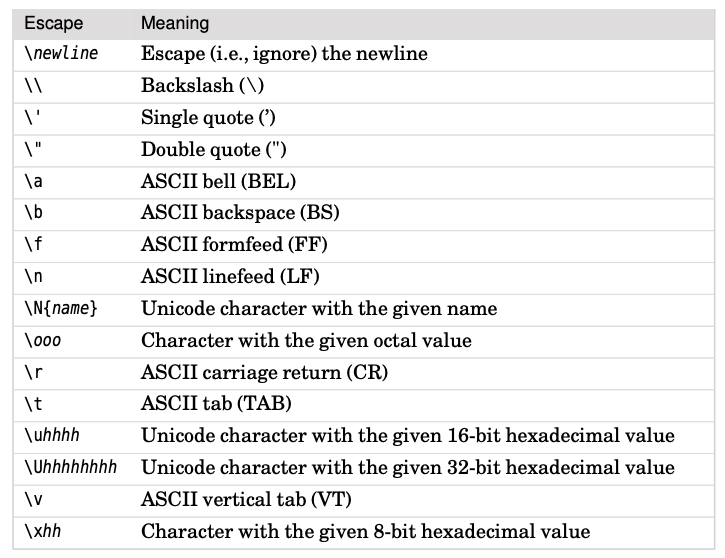
\includegraphics[width=\textwidth]{pics/escapes}
  \caption{Python's string escapes }
  \label{fig:escapes}
\end{figure}

In some situations --- for example, when writing regular expressions --- we need to create strings with lots of literal backslashes.
This can be inconvenient since each one must be escaped:
\begin{lstlisting}

import re
phone1 = re.compile("^((?:[(]\\d+[)])?\\s*\\d+(?:-\\d+)?)$")
\end{lstlisting}


The solution is to use \keyword{raw} strings.
These are quoted or triple quoted strings whose first quote is preceded by the letter \verb|r|.
Inside such strings all characters are taken to be literals, so no escaping is necessary.

\begin{lstlisting}

phone2 = re.compile(r"^((?:[(]\d+[)])?\s*\d+(?:-\d+)?)$")
\end{lstlisting}



\begin{lstlisting}

>>>'\N{euro sign}'
'€'
\end{lstlisting}



If we want to know the Unicode code point for a particular character in a string, we can use the built-in \verb|ord()| function:
\begin{lstlisting}

>>> ord('€')
8364
>>> hex(ord('€'))
'0x20ac'
>>> '\u20ac'
'€'
\end{lstlisting}


we can convert any integer that represents a valid code point into the corresponding Unicode character using the built-in \verb|chr()| function:

\begin{lstlisting}

>>> chr(8734)
'∞'
>>> chr(8364)
'€'
>>> ascii('€')
"'\\u20ac'"
\end{lstlisting}



\subsection{Comparing strings}

Strings support the usual comparison operators <, <=, ==, !=, >, and >=.
These operators compare strings byte by byte in memory.

\subsection{Slicing and striding strings}

\begin{lstlisting}

s = "Light ray"
\end{lstlisting}

Figure \ref{fig:string-index-position} shows all the valid index postions for string \verb|s|.

\begin{figure}[!ht]
  \centering
  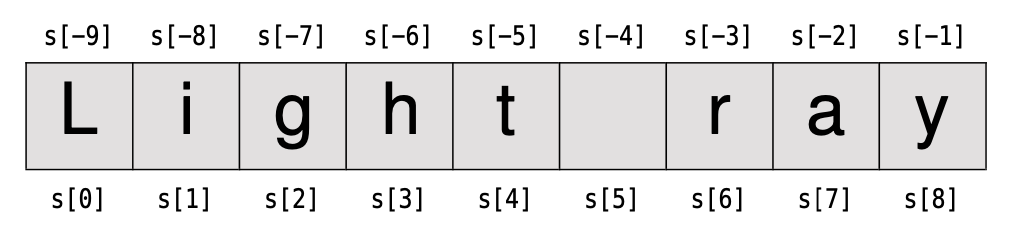
\includegraphics[width=\textwidth]{pics/string-index-position}
  \caption{String index position}
  \label{fig:string-index-position}
\end{figure}

The slice operator has three syntaxes:
\begin{verbatim}
seq[start]
seq[start:end]
seq[start:end:step]
\end{verbatim}


Using \verb|+| to concatenate and \verb|+=| to append is not particularly efficient when String
many strings are involved.
For joining lots of strings it is usually best to use the \verb|str.join()| method.



\subsection{String operators and methods}

Since strings are immutable sequences, all the functionality that can be used with imuutable sequences can be used with strings.

\begin{itemize}
\item membership (in)
\item concatenation (+)
\item appedning (+=)
\item replication (*)
\item augmented assignment replication (*=)
\end{itemize}


There are some common string methods:
\begin{description}
\item[s.capitalize()] 
\item[s.lower()] 
\item[s.title()] 
\item[s.upper()] 
\item[s.swapcase()] 
\item[s.center(width, char)]
\item[s.ljust(width, char)] 
\item[s.rjust(width, char)] 
\item[s.count(t, start, end)] 
\item[s.encode(encoding, err)] 
\item[s.startswith(x, start, end)] 
\item[s.endswith(x, start, end)] 
\item[s.expandtabs(size)] 
\item[s.find(t, start, end)] 
\item[s.index(t, start, end)] 
\item[s.format(...)] 
\item[s.isalnum()] 
\item[s.isalpha()] 
\item[s.isdecimal()] 
\item[s.isdigit()] 
\item[s.isidentifier()] 
\item[s.islower()]
\item[s.istitle()] 
\item[s.isupper()] 
\item[s.isnumeric()] 
\item[s.isprintable()] 
\item[s.isspace()] 
\item[s.join(seq)] 
\item[s.partition(t)] 
\item[s.replace(t, u, n)] 
\item[s.split(t, n)] 
\item[s.splitlines(f)] 
\item[s.strip(chars)] 
\item[s.maketrans()] 
\item[s.translate()] 
\item[s.zfill(w)] 
\end{description}

\subsection{String formatting with the str.format() method}

The \verb|str.format()| method returns a new string with the replacement fields in its string replaced with its arguments suitablely formatted.


\begin{lstlisting}

>>> "{0} {1} {2}".format("Hello", 'world', 'mike')
'Hello world mike'
\end{lstlisting}


Each replacement field is identified by a field name in braces.
If the field name is a simple integer, it is taken to be the index position of one of the arguments passed to \verb|str.format()|.


If we need to include braces inside format strings, we can do so by doubling them up.
\begin{lstlisting}

>>> 'just {{{0}}}'.format('brace')
'just {brace}'
\end{lstlisting}



The replacement field can have any of the following general syntaxes:
\begin{verbatim}
{field_name}
{field_name!conversion}
{field_name:format_specification}
{field_name!conversion:format_specification}
\end{verbatim}


\subsection{Field names}

A field name can be either an integer corresponding to one of the \verb|str.format()| method’s arguments, or the name of one of the method’s keyword arguments.

\begin{lstlisting}

>>> '{who} solve a leetcode problem every {0} days'.format(1, who='Mike')
'Mike solve a leetcode problem every 1 days'
\end{lstlisting}


Notice that in an argument list, keyword arguments always come after positional arguments.



If the arguments are collections data types like lists or dictionaries, or have attributes, we can access the part using [] or . notation.


\begin{lstlisting}

>>> stock = ["paper", "envelopes", "notepads"] 
>>> "We have {0[1]} and {0[2]} in stock".format(stock)
'We have envelopes and notepads in stock'

>>> d = dict(animal="elephant", weight=12000)
>>> "The {0[animal]} weighs {0[weight]}kg".format(d) 
'The elephant weighs 12000kg'

>>> "math.pi=={0.pi}".format(math) 
'math.pi==3.14159265359
\end{lstlisting}




The local variables that are currently in scope are available from the built-in \verb|locals()| function.
This function returns a dictionary whose keys are local variable names and whose values are references to the variables' values.
We can use \keyword{mapping unpacking} to feed this dictionary into the \verb|str.format()| method.
The mapping unpacking operator is \verb|**| and it can be applied to a mapping (such as dictionary) to produce a key-value list suitable for passing to a function.
For example:
\begin{lstlisting}

>>> element = "Silver"
>>> number = 47
>>> "Element {number} is {element}".format(**locals()) 
'Element 47 is Silver'
\end{lstlisting}




\subsection{conversions}

\begin{lstlisting}

>>> decimal.Decimal("3.4084") 
Decimal('3.4084')
>>> print(decimal.Decimal("3.4084")) 
3.4084
\end{lstlisting}


The first is in representational form.
The purpose of this form is to provide a string which if interpreted by Python would re-create the ojbect it represents.
Not all objects can provide a reproducing representation, in which case they provide a string enclosed in angle brackets.
For example \verb|"module 'sys' (built-in)>"|.

The second is in its string form.
This form is aimed at human readers, so the concern is to show something that makes sense to people.
If a data type doesn’t have a string form and a string is required, Python will use the representational form.


Python’s built-in data types know about \verb|str.format()|, and when passed as an argument to this method they return a suitable string to display themselves.
In addition, it is possible to override the data type’s normal behavior and force it to provide either its string or its representational form.
This is done by adding a conversion specifier to the field.
Currently there are three such specifiers:
\begin{itemize}
\item \verb|s| to force string form, 
\item \verb|r| to force representational for
\item \verb|a| to for representational form but only using ASCII characters.
\end{itemize}


\begin{lstlisting}

>>> "{0}  {0!s}  {0!r}  {0!a}  {1!r}  {1!a}".format(decimal.Decimal(1), "你好")
"1  1  Decimal('1')  Decimal('1')  '你好'  '\\u4f60\\u597d'"
\end{lstlisting}



\subsection{Format specifications}

\subsubsection{Specification for string}

For strings, the things that we can control are:
\begin{itemize}
\item the fill character, 
\item the alignment within the field, and 
\item the minimum and 
\item maximum field widths.
\end{itemize}

\begin{tcolorbox}
\begin{verbatim}
: fill     align        min_width   .max_width
            < for left
            > for right
            ^ for center
\end{verbatim}
\end{tcolorbox}


\begin{lstlisting}

>>> s = "The sword of truth"
>>> '{0}'.format(s)
'The sword of truth'
>>> '{0:25}'.format(s)
'The sword of truth       '
>>> '{0:>25}'.format(s)
'       The sword of truth'
>>> '{0:->25}'.format(s)
'-------The sword of truth'
>>> '{0:.<25}'.format(s)     # the left alignment can not be omitted
'The sword of truth.......'
>>> '{0:.10}'.format(s)
'The sword '
\end{lstlisting}


\subsubsection{Specification for integer}

For integers, the format specification allows us to control:
\begin{itemize}
\item the fill character, 
\item the alignment within the field, 
\item the sign, 
\item whether to use a nonlocale-aware comma separator to group digits, 
\item the minimum field width, and 
\item the number base.
\end{itemize}

\begin{tcolorbox}
\begin{verbatim}
: fill  alignment      sign             #      width   ,         type
        = pad between  + force sign;   prifix          use       b,c,d 
        sign and       - sign if       ints            commas    n,o,x,
        digits         needed;         with            for       X  
        for numbers    " " space or    0b, 0o,         grouping  
                       - as            or 0x  
                       appropriate
\end{verbatim}
\end{tcolorbox}


\begin{lstlisting}

>>> '{0:0=12}'.format(-1234)
'-00000001234'

>>> "[{0: }] [{1: }]".format(539802, -539802) # space or - sign 
'[ 539802] [-539802]'
>>> "[{0:+}] [{1:+}]".format(539802, -539802) # force sign 
'[+539802] [-539802]'
>>> "[{0:-}] [{1:-}]".format(539802, -539802) # - sign if needed 
'[539802] [-539802]'

>>> "{0:b} {0:o} {0:x} {0:X}".format(123)
'1111011 173 7b 7B'
>>> "{0:#b} {0:#o} {0:#x} {0:#X}".format(123)
'0b1111011 0o173 0x7b 0X7B'

>>> '{0:,}'.format(1234567890)
'1,234,567,890'
\end{lstlisting}


The last format character \verb|n| has the same effect as d when given an integer.
What makes \verb|n| special is that it respects the current locale and will use locale-specific decimal separator
and grouping separator in the output it produces.
The default locale is called the C locale, and for this the decimal and grouping characters are a period and an empty string.


\begin{lstlisting}

>>> import locale
>>> x = 1234567890
>>> locale.setlocale(locale.LC_ALL, 'C')
'C'
>>> '{:n}'.format(x)
'1234567890'
>>> locale.setlocale(locale.LC_ALL, 'en_US.UTF-8')
'en_US.UTF-8'
>>> '{:n}'.format(x)
'1,234,567,890'
>>> locale.setlocale(locale.LC_ALL, 'de_DE.UTF-8')
'de_DE.UTF-8'
>>> '{:n}'.format(x)
'1234567890'
\end{lstlisting}



\subsubsection{Specification for floating}


For floating-point numbers, the format specification gives us control over:
\begin{itemize}
\item the fill character, 
\item the alignment within the field, 
\item the sign, 
\item whether to use a non-locale aware comma separator to group digits, 
\item the minimum field width, 
\item the number of digits after the decimal place, and 
\item whether to present the number in standard or exponential form, or as a percentage.
\end{itemize}

\begin{tcolorbox}
\begin{verbatim}
: fill  alignment  sign  width  ,  .precision      type
                                   number of       e,E,f,
                                   decimal places  g,G,n,
                                                   %
\end{verbatim}
\end{tcolorbox}


\begin{itemize}
\item e for exponential form with lowercase e
\item E for exponential form with lowercase E
\item f for standard floating-point form
\item g for ``general'' form—this is the same as f unless the number is very large, in which case it is the same as e
\item G is is almost the same as g, but uses either f or E
\item \% for percentage
\end{itemize}


\begin{lstlisting}

>>> '{0:12.2e}'.format(math.pi)
'    3.14e+00'
>>> '{0:12.2f}'.format(math.pi)
'        3.14'
>>> '{:,.6f}'.format(1234567890.1234567890)
'1,234,567,890.123457'
>>> "{:,.4f}".format(3.59284e6-8.984327843e6j) 
'3,592,840.0000-8,984,327.8430j'
\end{lstlisting}





\subsubsection{Character encodings}

Unicode assigns every character to an integer --- called a \keyword{code point} in Unicode-speak.
Nowadays, Unicode is usually stored both on disk and in memory using UTF-8, UTF-16, or UTF-32.
The first of these, UTF-8, is backward compatible with 7-bit ASCII since its first 128 code points are represented by single-byte values that are the same as the 7-bit ASCII character values.
To represent all the other Unicode characters, UTF-8 uses two, three, or more bytes per character.


A lot of other software, such as Java, uses UCS-2 (which in modern form is the same as UTF-16).
This representation uses two or four bytes per character, with the most common characters represented by two bytes.
The UTF-32 representation (also called UCS-4) uses four bytes per character.
Using UTF-16 or UTF-32 for storing Unicode in files or for sending over a network connection has a potential pitfall: If the data is sent as integers then the endianness matters.
One solution to this is to precede the data with a byte order mark so that readers can adapt accordingly.
This problem doesn’t arise with UTF-8, which is another reason why it is so popular.


Python represents Unicode using either UCS-2 (UTF-16) format, or UCS-4 (UTF-32) format.
In fact, when using UCS-2, Python uses a slightly simplified version that always uses two bytes per character and so can only represent code points up to 0xFFFF.
When using UCS-4, Python can represent all the Unicode code points.
The maximum code point is stored in the read-only sys.maxunicode attribute—if its value is 65535, then Python was compiled to use UCS-2; if larger, then Python is using UCS-4.




\chapter{Collection data types}

\section{Sequence types}

\begin{tcolorbox}
  A \keyword{sequence} type is one that support:
  \begin{itemize}
  \item the membership operator (\verb|in|)
  \item the size function (\verb|len()|) 
  \item slices ([]) 
  \item and is iterable.
  \end{itemize}
  Python provides five built-in sequence types:
  \begin{itemize}
  \item bytearray
  \item bytes
  \item list
  \item str
  \item tuple
  \end{itemize}
  When iterated, all of these sequences provide their items in order.
\end{tcolorbox}



\subsection{Tuples}

Tuples are immutable.
Tuples are able to hold any items of any data type, including collection types such as tuples and lists, since what they really hold are object references.

Tuples provide just two methods, \verb|t.count(x)| and \verb|t.index(x)|.

\begin{tcolorbox}
  tuple coding style:
  omit parentheses:
  \begin{itemize}
  \item tuples on the left-hand size of a binary operator
  \item on the right-hand size of a unary statement
  \end{itemize}
  other cases with parentheses.

  \begin{lstlisting}

a, b = (1, 2)  # left of binary operator
del a, b       # right of unary operator
  \end{lstlisting}

\end{tcolorbox}


When we have a sequences on the right-hand side of an assignment, and
we have a tuple on the left-hand side,
we say that the right-hand side has been \keyword{unpacked}.
Sequence unpacking can be used to swap values, for example:
\begin{lstlisting}

a, b = (b, a) # or a, b = b, a
# the parentheses here are for code style

for x, y in ((3, 4), (5, 12), (28, -45):
    print(math.hypot(x, y))
\end{lstlisting}



\subsection{Named tuples}


A named tuple behaves just like a plain tuple, and has the same performance characteristics.
What it adds is the ability to refer to items in the tuple by name as well as by index position.


\begin{lstlisting}

import collections

Fullname = collections.namedtuple('Fullname',
                                  'firstname middlename lastname')
persons = []
persons.append(Fullname('Mike', 'Ming', 'Chyson'))
persons.append(Fullname('Alfred', 'Bernhard', 'Nobel'))
for person in persons:
    print('{firstname} {middlename} {lastname}'.format(**person._asdict()))

\end{lstlisting}



\subsection{Lists}

List are mutable.
Since all the items in a list are really object references, lists can hold items of any data type, including collection types such as lists and tuples.


Although we can use the slice operator to access items in a list, in some situations we want to take two or more pieces of a list in one go.
This can be done by sequence unpacking.
Any iterable (lists, tuples, etc.) can be unpacked using the sequence unpacking operator, an asterisk or star (*).
When used with two or more variables on the left-hand side of an assignment, one of which is preceded by *, items are assigned to the variables, with all those left over assigned to the starred variable.
Here are some examples:

\begin{lstlisting}

>>> a = list(range(10))
>>> first, *last = a
>>> print(first, last)
0 [1, 2, 3, 4, 5, 6, 7, 8, 9]
>>> 
>>> first, *middle, last = a
>>> print(first, middle, last)
0 [1, 2, 3, 4, 5, 6, 7, 8] 9
>>> 
>>> *first, last = a
>>> print(first, last)
[0, 1, 2, 3, 4, 5, 6, 7, 8] 9
\end{lstlisting}



List methods:
\begin{description}
\item[list.append(x)] 
\item[list.count(x)] 
\item[list.extend(m)] 
\item[list += m] 
\item[list.index(x, start, end)] 
\item[list.insert(i, x)] 
\item[list.pop()] Returns and removes the rightmost item of list
\item[list.pop(i)] 
\item[list.remove(x)] Removes the leftmost occurrence of item x from list
\item[list.reverse()] Reverses list in-place
\item[list.sort(...)] Sorts list in-place
\end{description}


Individual items can be replaced in a list by assigning to a particular index position.
Entire slices can be replaced by assigning an iterable to a slice.
The slice and the iterable don't have to be the same length.
In all cases, the slice's items are removed the the iterable's items are inserted.

\begin{lstlisting}

>>> nums = [0, 1, 2, 3, 4, 5, 6]
>>> nums[0] = 100
>>> nums
[100, 1, 2, 3, 4, 5, 6]
>>> nums[2:2] = [200]    # same to nums.insert(2, 200)
>>> nums
[100, 1, 200, 2, 3, 4, 5, 6]
>>> nums[2:4] = [10, 11, 12, 13, 14]
>>> nums
[100, 1, 10, 11, 12, 13, 14, 3, 4, 5, 6]
\end{lstlisting}


In lists, striding allows us to access every n-th item which can often be useful.
For example:
\begin{lstlisting}

>>> x = list(range(1, 11))
>>> x
[1, 2, 3, 4, 5, 6, 7, 8, 9, 10]
>>> x[1::2] = [0] * len(x[1::2])
>>> x
[1, 0, 3, 0, 5, 0, 7, 0, 9, 0]
\end{lstlisting}


\begin{lstlisting}
>>> x = list(range(-5, 5))
>>> x
[-5, -4, -3, -2, -1, 0, 1, 2, 3, 4]
>>> x.sort(key=lambda x: x**2)
>>> x
[0, -1, 1, -2, 2, -3, 3, -4, 4, -5]
\end{lstlisting}




For inserting items, lists perform best when items are added or removed at the end (\verb|list.append(), list.pop()|).
The worst performance occurs when we search for items in a list, for example, using \verb|list.remove()| or \verb|list.index()|, or using \verb|in| for membership testing.
If fast searching or membership testing is required, a \verb|set| or a \verb|dict| may be a more suitable collection choice.
Alternatively, lists can provide fast searching if they are kept in order by sorting them and using a binary search (provided by the \verb|bisect| module), to find items. 


\subsection{List comprehensions}

A \keyword{list comprehension} is an expression and a loop with optional condition enclosed in brackets where the loop is used to generate items for the list, and where the condition can filter out unwanted items.

\begin{verbatim}
[expression for item in iterable]
[expression for item in iterable if condition]
\end{verbatim}


\begin{lstlisting}
  leaps = [y for y in range(1900, 1940)
           if (y % 4) == 0 and y % 100 != 0) or (y % 400 == 0)]
\end{lstlisting}


If the generated list is very large, it may be more efficient to generate each item as it is needed rather than produce the whole list at once.
This can be achieved by using a generator rather than a list comprehension. 



\section{Set types}

\begin{tcolorbox}
A \keyword{set} is a collection data type that supports:
\begin{itemize}
\item the membership operator(\verb|in|),
\item the size function (\verb|len()|),
\item and is iterable.
\end{itemize}
Python provides two built-in set types:
\begin{itemize}
\item the mutable \verb|set| type
\item the immutable \verb|frozenset|
\end{itemize}
When iterated, set types provide their items in an arbitrary order.
\end{tcolorbox}



Only \keyword{hashable} objects may be added to a set.
Hashable objects are objects which have a \verb|__hash__()| special method whose return value is always the same thoughout the ojbect's lifetime, and which can be compared for equality using the \verb|__eq__()| special method.
(Special mehtods are methods whose name begins and ends with two underscores)



\subsection{Sets}

A \keyword{set} is an unordered collection of zero or more object references that refer to hashable objects.
Sets are mutable.
Sets always contain unique items --- adding duplicate items is safe but pointless.


\begin{figure}[!ht]
  \centering
  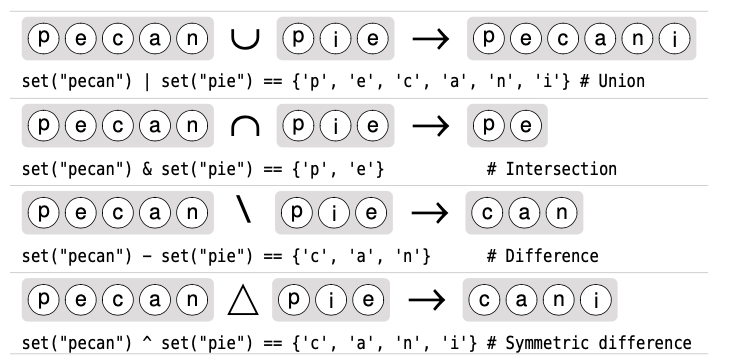
\includegraphics[width=\textwidth]{pics/standard-set-operators}
  \caption{Standard set operators}
  \label{fig:standard-set-operators}
\end{figure}


Set methods:
\begin{description}
\item[s.add(x)] 
\item[s.clear()] 
\item[s.copy()] 
\item[s.difference(t)] Same to s - t
\item[s.difference\_{}update(t)] Same to s -= t
\item[s.discard] Removes item x from set s if it is in s
\item[s.remove()] Removes item x from set s, or raises a KeyError exception if x is not in s
\item[s.intersection(t)] Same to s \& t
\item[s.intersection\_{}update(t)] Same to s \&= t
\item[s.isdisjoint(t)] Returns True if sets s and t have no items in common
\item[s.issubset(t)] Same to s <= t
\item[s.issuperset(t)] Same to s >= t
\item[s.pop()] Returns and remove a random item from set s, or raises a KeyError exception if s is empty
\item[s.symmetric\_{}difference(t)] Same to s \^{} t
\item[s.symmetric\_{}difference\_{}update(t)] Same to s\^{}= t
\item[s.union(t)] Same to s | t
\end{description}


Sets are used used for fast membership test and removring duplicated items.


\subsection{Set comprehensions}

\begin{verbatim}
{expression for item in iterable}
{expression for item in iterable if condition}
\end{verbatim}

\subsection{Frozen sets}

A frozen set is a set that, once created, cannot be changed.
Since frozen set are immutable, sets and frozen sets can contain frozen sets.



\section{Mapping types}

\begin{tcolorbox}
A \keyword{mapping} type is one that supports:
\begin{itemize}
\item the membership operator (in)
\item the size function (len())
\item is iterable 
\end{itemize}

Mappings are collection of key-value items and provide methods for accessing items and their keys and values.
\end{tcolorbox}

When iterated, unordered mapping types provide their items in an arbitrary order.


There are one built-in mapping types and two standard library's mapping types:
\begin{itemize}
\item dict
\item collections.defaultdict
\item collections.OrderedDict
\end{itemize}



\subsection{Dictionaries}

A \verb|dict| is an unordered collection of zero or more key–value pairs whose keys are object references that refer to hashable objects, and whose values are object references referring to objects of any type.
Dictionaries are mutable.

\begin{lstlisting}
>>> d = dict()
>>> d
{}
>>> d = {}
>>> d
{}
>>> d = {"hello": 1, "world": 2}
>>> d
{'hello': 1, 'world': 2}
>>> d = dict(hello=1, world=2)
>>> d
{'hello': 1, 'world': 2}
>>> d = dict([("hello", 1), ("world", 2)])
>>> d
{'hello': 1, 'world': 2}  
\end{lstlisting}



Dictionary methods:
\begin{description}
\item[d.clear()] 
\item[d.copy()] 
\item[d.fromkeys(s, v)] Returns a dict whose keys are the items in sequence s and whose values are None or v if v is given
\item[d.get(k)] Returns key k's associated value or None if k isn't in dict d
\item[d.get(k, v)] Returns key k's associated value, or v if k isn't in dict d
\item[d.items()] 
\item[d.keys()] 
\item[d.values()] 
\item[d.pop(k)] 
\item[d.pop(k, v)] 
\item[d.popitem()] Returns and removes an arbitrary (key, value) pair from dict d
\item[d.setdefault(k, v)] The same as the dict.get() method, except that if the key is not indict d,a new item is inserted with the key k, and with a value of None or of v if v is given
\item[d.update(a)] Adds every (key, value) pair from a that isn’t in dict d to d, and for every key that is in both d and a, replaces the corresponding value in d with the one in a --— a can be a dictionary, an iterable of (key, value) pairs, or keyword arguments
\end{description}



The \verb|dict.items()|, \verb|dict.keys()|, and \verb|dict.values()| methods all return dictionary views.
A dictionary view is effectively a read-only iterable object that appears to hold the dictionary’s items or keys or values, depending on the view we have asked for.


In general, we can simply treat views as iterables.
However, two things make a view different from a normal iterable.
One is that if the dictionary the view refers to is changed, the view reflects the change.
The other is that key and item views support some set-like operations.
Given dictionary view \verb|v| and \verb|set| or dictionary view \verb|x|, the supported operations are:
\begin{verbatim}
v & x  # intersection
v | x  # union
v - x  # difference
v ^ x  # symmetric difference
\end{verbatim}



\begin{lstlisting}
>>> d = {}.fromkeys("abcd", 3)
>>> d
{'a': 3, 'b': 3, 'c': 3, 'd': 3}
>>> s = set("abc")
>>> s
{'a', 'c', 'b'}
>>> d.keys() & s
{'a', 'c', 'b'}
>>> 
>>> d
{'a': 3, 'b': 3, 'c': 3, 'd': 3}
>>> d.setdefault('a')
3
>>> d
{'a': 3, 'b': 3, 'c': 3, 'd': 3}
>>> d.setdefault('z', 100)
100
>>> d
{'a': 3, 'b': 3, 'c': 3, 'd': 3, 'z': 100}  
  
\end{lstlisting}




\subsection{Dictionary comprehensions}

\begin{lstlisting}
{keyexpression: valueexpression for key, value in iterable}
{keyexpression: valueexpression for key, value in iterable if condition}
\end{lstlisting}


\begin{lstlisting}
import os

# filename: filesize
d = {name: os.path.getsize(name) for name in os.listdir('.') if os.path.isfile(name)}
print(d)

# revert dict
inserted_d = {v: k for k, v in d.items()}
print(inserted_d)  
\end{lstlisting}


\subsection{Default dictionaries}

Default dictionaries are dictionaries --- they have all the operators and methods that dictionaries provide.
What makes default dictionaries different from plain dictionaries is the way they handle missing keys.



When a default dictionary is created, we can pass in a \keyword{factory function}.
A factory function is a function that, when called, returns an object of a particular type.
All of Python’s built-in data types can be used as factory functions.
The factory function passed to a default dictionary is used to create default values for missing keys.


\begin{tcolorbox}
  Note that the \keyword{name} of a function is an object reference to the function --- so when we want to pass functions as parameters, we just pass the name.
  When we use a function with parentheses, the parentheses tell Python that the function should be called.
\end{tcolorbox}

\begin{lstlisting}
>>> words = collections.defaultdict(int)
>>> words
defaultdict(<class 'int'>, {})
>>> words['hello'] += 1
>>> words
defaultdict(<class 'int'>, {'hello': 1})
>>> words['hello'] += 1
>>> words
defaultdict(<class 'int'>, {'hello': 2})
>>> 
>>> de = collections.defaultdict(lambda : "Thanks to ")
>>> de
defaultdict(<function <lambda> at 0x7fa999a75a60>, {})
>>> de['Mike'] += 'Mike'
>>> de
defaultdict(<function <lambda> at 0x7fa999a75a60>, {'Mike': 'Thanks to Mike'})  
\end{lstlisting}


\subsection{Ordered dictionaries}
The ordered dictionaries type is \verb|collections.OrderedDict|
Ordered dictionaries store their items in the order in which they were inserted.
If we change an item's value, the order is not changed.


\begin{lstlisting}
d = collections.OrderedDict([('z', -4), ('e', 19), ('k', 7)])
for k in d:
    print(k, d[k])
    
tasks = collections.OrderedDict()
tasks[8031] = "Backup"
tasks[4027] = "Scan Email"
tasks[5733] = "Build System"
for k in tasks:
    print(k, tasks[k])  
\end{lstlisting}


If we want to move an item to the end, we must delete it and then reinsert it.
We can also call \verb|popitem()| to remove and return the last key–value item in the ordered dictionary; or we can call
\verb|popitem(last=False)|, in which case the first item will be removed and returned.



\section{Iterating and copying collections}

\subsection{Iterators and iterable operations and functions}

An \keyword{iterable} data type is one that can return each of its items one at a time.
Any object that has an \verb|__iter__()| method, or any sequence (i.e. an object that has a \verb|__getitem__()| method taking integer arguments starting from 0) is an iterable and can be provide an \keyword{iterator}.
An iterator is an object that provides a \verb|__next__()| method which returns each successive item in turn, and raises a \verb|StopIteration| exception when there are no more items.


The operators and functions that can be used with iterables:
\begin{description}
\item[s + t] Returns a sequence that is the concatenation of sequences s and t
\item[s * t] Returns a sequences that is int n concatenation of sequences s
\item[x in i] Returns True if item x is in iterable i
\item[all(i)] Returns True if every item in iterable i evalueates to True
\item[any(i)] Returns True if any item in iterable i evalueates to True
\item[enumerate(i, start)] Normally used in for ... in loops to provide a sequence of (index, item) tuples with indexes starting at 0 or start
\item[len(x)] 
\item[max(i, key)] Returns the biggest item in iterable i or the item with the biggest key(item) value if a key function is given
\item[min(i, key)] Returns the smallest item in iterable i or the item with the smallest key(item) value if a key function is given
\item[range(start, stop, step)] Returns an integer iterator.
\item[reversed(i)] Returns an iterator that returns the items from iterator i in reverse order
\item[sorted(i, key, reverse)] Return a list of the items from iterator i in sorted order; key is used to provide DSU (Decorate, Sort, Undecorate) sorting. If reverse is True the sorting is done in reverse order.
\item[sum(i, start)] Returns the sum of the items in iterable i plus start (which defaults to 0)
\item[zip(i1, ..., iN)] Returns an iterator of tuples using the iterators i1 to iN
\end{description}


The order in which items are returned depends on the underlying iterable.
In the case of lists and tuples, items are normally returned in sequential order starting from the first item (index position 0), but some iterators return the items in an arbitrary order --- for example, dictionary and set iterators.


The built-in \verb|iter()| function has two quite different behaviors.
\begin{itemize}
\item When given a collection data type or a sequence it returns an iterator for the oject it is passed --- or raise a \verb|TypeError| if the object cannot be iterable.
\item When given a callable (a function or method) and a sentinel value, the function passed in is called once at each iteration, returning teh function'sreturn value each time, or raising a \verb|StopIteration| exception if the return value equals the sentinel.
\end{itemize}




When we use a \verb|for item in iterable| loop, Python in effect calls \verb|iter(iterable)| to get an iterator.
This iterator's \verb|__next__()| method is then called at each loop iteration to get the next item, and when the \verb|StopIteration| exception is raised, it is caughted and the loop is terminated.



\begin{lstlisting}
# manner 1
product = 1
for i in [1, 2, 4, 8]:
    product *= i
print(product)


# manner 2
product = 1
i = iter([1, 2, 4, 8])
while True:
    try:
        product *= i
    except StopIteration:
        break
print(product)  
\end{lstlisting}



Any (finite) iterable, i, can be converted into a tuple by calling \verb|tuple(i)|, or can be converted into a list by calling \verb|list(i)|.




\begin{lstlisting}
>>> x = []
>>> for t in zip(range(-10, 0, 1), range(0, 10, 2), range(1, 10, 2)):
...     x += t
... 
>>> x
[-10, 0, 1, -9, 2, 3, -8, 4, 5, -7, 6, 7, -6, 8, 9]
>>> sorted(x)
[-10, -9, -8, -7, -6, 0, 1, 2, 3, 4, 5, 6, 7, 8, 9]
>>> sorted(x, reverse=True)
[9, 8, 7, 6, 5, 4, 3, 2, 1, 0, -6, -7, -8, -9, -10]
>>> sorted(x, key=abs)
[0, 1, 2, 3, 4, 5, 6, -6, -7, 7, -8, 8, -9, 9, -10]  
\end{lstlisting}


\begin{tcolorbox}
  A function's name is an object reference to the function;
  it is the parentheses that follow the name that tell Python to call the function.
\end{tcolorbox}


Python's sort algorithm is an adaptive stable mergesort that is both fast and smart, and it is especially well optimized for partially sorted lists.
The ``adaptive'' part means that the sort algorithm adapts to circumstances --- for example, taking advantage of partially sorted data.
The ``stable'' part means that the items that sort equally are not moved in relation to each other.
When sorting collections of itegers, strings, or other simple types their ``less than'' operator (<) is used.
Python can sort collections that contain collections, working recursively to any depth.



Lists can be sorted in-place using the \verb|list.sort()| method, which takes the same optinal arguments as \verb|sorted()|.


\subsection{Copying collections}

Since Python uses \keyword{object references}, when we use the assignment operator (+), no copying takes place.
If the right-hand operand is a literal such as a string or a number, the left-hand operand is set to be an object reference that refers to the in-memory object that holds the literal’s value.
If the right-hand operand is an object reference, the left-hand operand is set to be an object reference that refers to the same object as the right-hand operand.
One consequence of this is that assignment is very efficient.



For sequences, when we take a slice, the slice is always an independent copy of the items copied.
For dictionaries and sets, copying can be achived using \verb|dict.copy()| and \verb|set.copy()|.
In addition, the \verb|copy| module provides the \verb|copy.copy()| function that returns a copy of the object it is given.
Another way to copy the built-in collection types is to use the type as a function with the collection to be copied as its argument.




\begin{tcolorbox}
  Note, thought, that all of these copying techniques are \keyword{shallow} --- that is, only object references are copied and not the object themselves.
  For immutable data types like numbers and strings this has the same effect as copying, but for mutable data types such as nested collections this means that the object they refer to are referred to both by the original collection and by the copied collection.


  \begin{lstlisting}
    print('{:.^50}'.format('print(x,y)'))
    x = [53, 68, ['A', 'B', 'C']]
    y = x[:]
    print(x, y, sep='\n')
    
    print('{:.^50}'.format('print(x,y)'))
    y[1] = 40
    x[2][0] = 'Q'
    print(x, y, sep='\n')

    """
    ....................print(x,y)....................
    [53, 68, ['A', 'B', 'C']]
    [53, 68, ['A', 'B', 'C']]
    ....................print(x,y)....................
    [53, 68, ['Q', 'B', 'C']]
    [53, 40, ['Q', 'B', 'C']]
    """
  \end{lstlisting}
\end{tcolorbox}



If we really need independent copies of arbitrarily nested collections, we can deep-copy:
\begin{lstlisting}
import copy

x = [53, 68, ['A', 'B', 'C']]
y = copy.deepcopy(x)
y[1] = 40
x[2][0] = 'Q'
print('{:.^50}'.format('print(x,y)'))
print(x, y, sep='\n')

"""
....................print(x,y)....................
[53, 68, ['Q', 'B', 'C']]
[53, 40, ['A', 'B', 'C']]
"""
\end{lstlisting}







\chapter{Control structures and functions}

\section{Control structures}

\subsection{Conditional branching}
\begin{tcolorbox}
\begin{verbatim}
if boolean_expression1:
    suite1
elif boolean_expression2:
    suite2
...
elif boolean_expressionN:
    suiteN
else:
    else_suite
\end{verbatim}
  
\end{tcolorbox}



\keyword{conditional expression}:
\begin{tcolorbox}
\begin{verbatim}
expression1 if boolean_expression else expression2
\end{verbatim}
  
\end{tcolorbox}

One common programming pattern is to set a variable to a default value, and then change the value if necessary.


\begin{lstlisting}
  width = 100 + (10 if margin else 10)
  print('{} file{}'.format(count if count != 0 else 'no', 's' if count != 1 else ''))
\end{lstlisting}

\subsection{Looping}

\subsubsection{while loops}

\begin{tcolorbox}
\begin{verbatim}
while boolean_expression:
    while_suite
else:
    else_suite
\end{verbatim}
  
\end{tcolorbox}

As long as the \verb|boolean_expression| is \verb|True|, the \verb|while| block's suite is executed.
If the \verb|boolean_expression| is or becomes False, the loop terminates, and if the optional \verb|else| clause is present, its suite is executed.
If the loop does not terminate normally, any optional \verb|else| clause's suite is skipped.
That is, if the loop is broken out of due to a \verb|break| statement, or a \verb|return| statement, or if an exception is raised, the \verb|else| clause's suite is not executed.


\begin{lstlisting}
i = 0
while i < 100:
    i += 1
else:
    last = i
print(last)  # 100
\end{lstlisting}

\begin{lstlisting}
def list_find(lst, target):
    """
    Find the first target's index or -1 if not find.

    :param lst:
    :param target:
    :return: index of the target if found or -1 if not found
    """
    index = 0
    while index < len(lst):
        if lst[index] == target:
            break
        index += 1
    else:
        index = -1
    return index  
\end{lstlisting}




\subsubsection{for loops}
\begin{tcolorbox}

\begin{verbatim}
for expression in iterable:
    for_suite
else:
    else_suite
\end{verbatim}
  
\end{tcolorbox}

The rule to run \verb|else_suite| is same for while loop.

\begin{lstlisting}
def list_find2(lst, target):
    for index, x in enumerate(lst):
        if x == target:
            break
    else:
        index = -1
    return index  
\end{lstlisting}


\section{Exception handling}

\subsection{Catching and raising exceptions}

\begin{tcolorbox}
\begin{verbatim}
try:
    try_suite
except exception_group1 as variable1:
    except_suite1
...
except exception_groupN as variableN:
    except_suiteN
else:
    else_suite
finally:
    finally_suite
\end{verbatim}
  
\end{tcolorbox}


There must be at least one \verb|except| block, but both the \verb|else| and the \verb|finally| blocks are optional.
The \verb|else| block’s suite is executed when the \verb|try| block’s suite has finished normally --- but it is not executed if an exception occurs.
If there is a \verb|finally| block, it is always executed at the end.

Each \verb|except| clause’s exception group can be a single exception or a parenthesized tuple of exceptions. 

If an exception occurs in the \verb|try| block’s suite, each \verb|except| clause is tried in turn.
If the exception matches an exception group, the corresponding suite is executed.
To match an exception group, the exception must be of the same type as the (or one of the) exception types listed in the group, or the same type as the (or one of the) group’s exception types’ subclasses.



\begin{lstlisting}
def lst_find(lst, target):
    try:
        index = lst.index(target)
    except ValueError:
        index = -1
    return index  
\end{lstlisting}




Python offers a simpler \verb|try...finally| block:
\begin{tcolorbox}
\begin{verbatim}
try:
    try_suite
finally:
    finally_suite
\end{verbatim}
  
\end{tcolorbox}



\begin{lstlisting}
# remove black lines
def read_data(filename):
    lines = []
    fh = None
    try:
        fh = open(filename)
        for line in fh:
            if line.strip():
                lines.append(line)
    except (IOError, OSError) as err:
        print(err)
        return []
    finally:
        if fh is not None:
            fh.close()
    return lines  
\end{lstlisting}



\subsubsection{Rasing exceptions}

Exceptions provide a useful means of changing the flow of control.

There are three syntaxes for raising exceptions:
\begin{tcolorbox}

\begin{verbatim}
raise exception(args)
raise exception(args) from original_exception
raise
\end{verbatim}
  
\end{tcolorbox}

If we give the exception some text as its argument, this text will be output if the exception is printed when it is caught.
When the third syntax is used, \verb|raise| will reraise the currently active exception --- and if there isn't one it will raise a \verb|TypeError|.


\subsection{Custom exceptions}

Custom exceptions are custom data types (classes).
\begin{tcolorbox}
\begin{verbatim}
class exceptionName(baseException): pass
\end{verbatim}
  
\end{tcolorbox}

The base class should be \verb|Exception| or a class that inherits from \verb|Exception|.



One use of custom exceptions is to break out of deeply nested loops.

\begin{lstlisting}
def find_word(table, target):
    found = False
    for row, record in enumerate(table):
        for column, field in enumerate(record):
            for index, item in enumerate(field):
                if item == target:
                    found = True
                    break
            if found:
                break
        if found:
            break

    if found:
        print('found at ({}, {}, {})'.format(row, column, index))
    else:
        print('not found')


def find_word2(table, target):
    class FoundException(Exception):
        pass

    try:
        for row, record in enumerate(table):
            for column, field in enumerate(record):
                for index, item in enumerate(field):
                    if item == target:
                        raise FoundException
    except FoundException:
        print('found at ({}, {}, {})'.format(row, column, index))
    else:
        print('not found')  
\end{lstlisting}


\begin{verbatim}
BaseException
 +-- SystemExit
 +-- KeyboardInterrupt
 +-- GeneratorExit
 +-- Exception
      +-- StopIteration
      +-- StopAsyncIteration
      +-- ArithmeticError
      |    +-- FloatingPointError
      |    +-- OverflowError
      |    +-- ZeroDivisionError
      +-- AssertionError
      +-- AttributeError
      +-- BufferError
      +-- EOFError
      +-- ImportError
      |    +-- ModuleNotFoundError
      +-- LookupError
      |    +-- IndexError
      |    +-- KeyError
      +-- MemoryError
      +-- NameError
      |    +-- UnboundLocalError
      +-- OSError
      |    +-- BlockingIOError
      |    +-- ChildProcessError
      |    +-- ConnectionError
      |    |    +-- BrokenPipeError
      |    |    +-- ConnectionAbortedError
      |    |    +-- ConnectionRefusedError
      |    |    +-- ConnectionResetError
      |    +-- FileExistsError
      |    +-- FileNotFoundError
      |    +-- InterruptedError
      |    +-- IsADirectoryError
      |    +-- NotADirectoryError
      |    +-- PermissionError
      |    +-- ProcessLookupError
      |    +-- TimeoutError
      +-- ReferenceError
      +-- RuntimeError
      |    +-- NotImplementedError
      |    +-- RecursionError
      +-- SyntaxError
      |    +-- IndentationError
      |         +-- TabError
      +-- SystemError
      +-- TypeError
      +-- ValueError
      |    +-- UnicodeError
      |         +-- UnicodeDecodeError
      |         +-- UnicodeEncodeError
      |         +-- UnicodeTranslateError
      +-- Warning
           +-- DeprecationWarning
           +-- PendingDeprecationWarning
           +-- RuntimeWarning
           +-- SyntaxWarning
           +-- UserWarning
           +-- FutureWarning
           +-- ImportWarning
           +-- UnicodeWarning
           +-- BytesWarning
           +-- ResourceWarning
\end{verbatim}


\section{Costom functions}

Functions are a means by which we can package up and parameterize functionality.
Four kinds of functions can be created in Python:
\begin{itemize}
\item global functions
\item local functions
\item lambda functions
\item methods
\end{itemize}


Global objects (including functions) are accessible to any code in the same module (i.e., the same .py file) in which the object is created.
Global objects can also be accessed from other modules.

Local functions (also called nested functions) are functions that are defined inside other functions.
These functions are visible only to the function where they are defined.




Lambda functions are expressions, so they can be created at their point of use; however, they are much more limited than normal functions.

Methods are functions that are associated with a particular data types and can be used only in conjunction with the data type.



The general syntax for creating a (global or local) function is:
\begin{tcolorbox}
\begin{verbatim}
def function_name(parameters):
    suite
\end{verbatim}
\end{tcolorbox}

\begin{lstlisting}
def my_sum(a, b, c=1):
    return a + b + c


print(my_sum(1, 2, 3)) # 6
print(my_sum(1, 2))    # 4
\end{lstlisting}


\verb|a,b| is called \keyword{positional arguments}, because each argument passed is set as the value of the parameter in the corresponding position.
\verb|c| is called \keyword{keyword arguments}, because each argument is passed by keyword not order.


When default values are given they are created at the time the \verb|def| statement is executed (i.e., when the function is created), not when the function is called.
For immutable arguments like numbers and strings this doesn’t make any difference, but for mutable arguments a subtle trap is lurking.

\begin{lstlisting}
def append_if_even(x, lst=[]):
    if x % 2 == 0:
        lst.append(x)
    return lst


def append_if_even2(x, lst=None):
    lst = [] if lst is None else lst
    if x % 2 == 0:
        lst.append(x)
    return lst


for i in range(3):
    result1 = append_if_even(i)
    result2 = append_if_even2(i)
    print(f'{result1=},{i=}')
    print(f'{result2=},{i=}')  

# result1=[0],i=0
# result2=[0],i=0
# result1=[0],i=1
# result2=[],i=1
# result1=[0, 2],i=2
# result2=[2],i=2
\end{lstlisting}


This idiom of having a default of \verb|None| and creating a fresh object should be used for dictionaries, lists, sets, and any other mutable data types that we want to use as default arguments.


\subsection{Names and docstrings}

\begin{tcolorbox}
  A few rules of good names:
  \begin{itemize}
  \item Use a naming scheme, and use it consistently.
    For example:
    \begin{itemize}
    \item \verb|UPPERCASE| for constants
    \item \verb|TitleCase| for classes
    \item \verb|camelCase| for GUI functions and methods
    \item \verb|lowercase| or \verb|lowercase_with_underscores| for everything else
    \end{itemize}
  \item For all names, avoid abbreviations, unless they are both standardized and widely used.
  \item Be proprotional with variable and parameter names: \verb|x| is a perfectly good name for an x-coordinate and \verb|i| is fine for a loop counter, but in general the name should be long enough to be descriptive.
  \item Functions and methods should have names that say what they do or what they return, but never how they do it --- since that might change.
  \end{itemize}
\end{tcolorbox}



We can add documentation to any function by using a \keyword{docstring} --- this is simply a string that comes immediately after the \verb|def| line, and before the function’s code proper begins.

\begin{lstlisting}
def shorten(text, length=25, indicator="..."):
    """Returns text or a truncated copy with the indicator added

    text is any string; length is the maximum length of the returned
    string (including any indicator); indicator is the string added at
    the end to indicate that the text has been shortened

    >>> shorten("Second Variety")
    'Second Variety'
    >>> shorten("Voices from the Street", 17)
    'Voices from th...'
    >>> shorten("Radio Free Albemuth", 10, "*")
    'Radio Fre*'
    """
    if len(text) > length:
        text = text[:length - len(indicator)] + indicator
    return text  
\end{lstlisting}

\begin{tcolorbox}
It is not unusual for a function or method’s documentation to be longer than the function itself.
One convention is to make
the first line of the docstring a brief one-line description,
then have a blank line followed by a full description, and then
to reproduce some examples as they would appear if typed in interactively.
\end{tcolorbox}


\subsection{Argument and parameter unpacking}
We can use sequence unpacking operator(*) to supply positional arguments and or mapping unpacking operator(**) to keyword arguemnts.
\begin{lstlisting}
def my_sum(a, b, c=1):
    return a + b + c

print(my_sum(*[1, 2, 3, 4][:3]))    # 6
print(my_sum(*[1, 2], **{'c': 3}))  # 6  
\end{lstlisting}


We can also use the sequence unpacking operator in a function's parameter list.
This is useful when we want to create functions that can take a variable number of positional arguments.

\begin{lstlisting}
def product(*args):
    result = 1
    for arg in args:
        result *= arg
    return result  
\end{lstlisting}

Having the * in front means that inside the function the \verb|args| parameter will be a \keyword{tuple} with its itmes set to however many positional arguments are given.


\begin{lstlisting}
def product(*args):
    result = 1
    for arg in args:
        result *= arg
    return result


print(product(*list(range(1, 10))))  # 362880
print(math.factorial(9))             # 362880
\end{lstlisting}



\begin{lstlisting}
# It is also possible to use * as a “parameter” in its own right.
# This is used to signify that there can be no positional arguments after the *.
def heron(a, b, c, *, units='square meters'):
    s = (a + b + c) / 2
    area = math.sqrt(s * (s - a) * (s - b) * (s - c))
    return f'{area} {units}'


print(heron(25, 24, 7))
print(heron(41, 9, 40, units="sq. inches"))
print(heron(25, 24, 7, "sq. inches"))   # TypeError
\end{lstlisting}



We can also use the mapping unpacking operator with parameters.
This allows us to create functions that will accept as many keyword arguments as are given.

\begin{lstlisting}
def print_dict(**kwargs):
    for key in sorted(kwargs):
        print(f'{key:10} : {kwargs[key]}')


print_dict(**{str(i): f'{100 * i:3}%' for i in range(10)})  

# 0          :   0%
# 1          : 100%
# 2          : 200%
# 3          : 300%
# 4          : 400%
# 5          : 500%
# 6          : 600%
# 7          : 700%
# 8          : 800%
# 9          : 900%
\end{lstlisting}

\begin{lstlisting}
def print_args(*args, **kwargs):
    for i, arg in enumerate(args):
        print("positional argument {0} = {1}".format(i, arg))
    for key in kwargs:
        print("keyword argument {0} = {1}".format(key, kwargs[key]))


print_args(*list(range(10)), **locals())  
\end{lstlisting}




\subsection{Accessing variables in the global scope}

\begin{tcolorbox}
There are two ways to create a global variable:
\begin{itemize}
\item Object defined in \verb|.py| level is global variables.
\item variables defined with \verb|global| keyword.
\end{itemize}
Others are local variables.
\end{tcolorbox}

\begin{lstlisting}
AUTHOR = 'Mike'  # global


def say_hello():  # global
    global language  # global
    language = 'fr'
    text = 'hello'  # local
    print(text)


class MyException(Exception):  # global
    pass


say_hello()
print(language)  
\end{lstlisting}


\subsection{Lambda functions}

Lambda functions are functions created using the following syntax:
\begin{tcolorbox}
\begin{verbatim}
lambda parameters: expression
\end{verbatim}
\end{tcolorbox}


The \keyword{parameters} are optinal, and if supplied they are normally just comma-separated variable names, that is, positional arguments, although the complement argument syntax supported by \verb|def| statements can be used.
The \verb|expression| can not contain \keyword{branches} or \keyword{loops} (although conditional expressions are allowed), and can not have a \verb|return| (or \verb|yield|) statment.
The result of a \verb|lambda| expression is an anonymous function.
When a lambda function is called it returns the result of computing the \verb|expression| as its result.



\begin{lstlisting}
lst = list(range(-3, 3))
print(lst)
print(sorted(lst, key=lambda x: x ** 2))
print(sorted(lst, key=lambda key=None: key ** 2))  # seldom used

# [-3, -2, -1, 0, 1, 2]
# [0, -1, 1, -2, 2, -3]
# [0, -1, 1, -2, 2, -3]
\end{lstlisting}


\begin{lstlisting}
s = lambda x: '' if x == 1 else 's'  # use def instead
print(s(1))  #
print(s(2))  # s

p = lambda key='hello': print(key)  # use def instead
p('world')  # world  
\end{lstlisting}


There are two common usage for lambda functions:
\begin{itemize}
\item key function
\item default value
\end{itemize}

\begin{lstlisting}
  sorted(lst, key=lambda x: x ** 2))
  message_dict = collections.defaultdict(lambda: 'No message avaiable')
\end{lstlisting}





\subsection{Assertions}

Preconditions and postconditions can be specified using \verb|assert| statements:
\begin{tcolorbox}
\begin{verbatim}
assert boolean_expression, optional_expression
\end{verbatim}
\end{tcolorbox}



If the \verb|boolean_expression| evaluates to \verb|False| an \verb|AssertionError| exception is raised.
If the optional \verb|optional_expression| is given, it is used as the argument to the \verb|AssertionError| exception.


\begin{lstlisting}
def product(*args):
    assert all(args), "0 argument"
    result = 1
    for arg in args:
        result *= arg
    return result

\end{lstlisting}

\begin{tcolorbox}
  Note:
  Assertions are designed for developers, not end-users.
  Once a program is readly for public release, we can tell Python not to execute \verb|assert| statements.
  This can be done with:
  \begin{itemize}
  \item -0 option in commandline, python -O program.py
  \item set the \verb|PYTHONOPTIMIZE| environment variable to O.
  \end{itemize}

  We can use -OO option to strip out both \verb|assert| statements and docstrings.
  However, there is no environment variable for setting this option.
\end{tcolorbox}




















































































\chapter{Modules}

\begin{itemize}
\item Functions allow us to parcel up pieces of code so that they can be reused throughout a program.
\item Modules provides a means of collecting sets of functions together so that they can be used by any number of programs.
\item Packages group sets of modules because their moduels provide related functionality or because they depend on each other.
\end{itemize}


\begin{tcolorbox}
  It is important to be aware of what the library has to offer, since using predefined functionality makes programming much faster than creating everything from scratch.
\end{tcolorbox}


\section{Modules and packages}

Several syntaxes can be used when importint:
\begin{tcolorbox}
\begin{verbatim}
import importable
import importable1, importable2, ..., importableN
import importable as preferred_name

from importable import object as preferred_name
from importable import object1, object2, ..., objectN
from importable import *
\end{verbatim}
\end{tcolorbox}


In the last syntex, the * means ``import everything that is not private'',
which in practical terms means
either every object in the module is imported except for those whose names begin with a leading underscore, or,
if the module has a global \verb|__all__| variable that holds a list of names, that all the objects named in the \verb|__all__| variable are imported.






\begin{tcolorbox}
  How does Python know where to look for the modules and packages that are imported?

  The built-in \verb|sys| module has a list called \verb|sys.path| that holds a list of the directories that consistutes the \keyword{Python path}.
  The first directory is the directory that contains the program itself, even if the program was invoked from another directory.
  If the PYTHONPATH environment variable is set, the paths specified in it are the next ones in the list.
  The final paths are those needed to access Python’s standard library --- these are set when Python is installed.

  When we first import a module, if it isn’t built-in, Python looks for the module in each path listed in \verb|sys.path| in turn. 
\end{tcolorbox}


\begin{figure}[!ht]
  \centering
  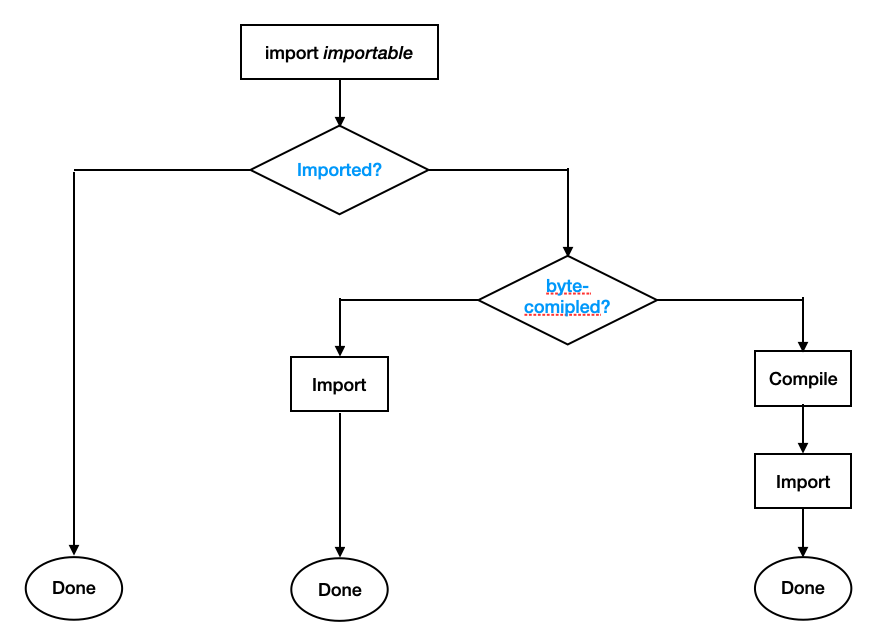
\includegraphics[width=\textwidth]{pics/import}
  \caption{Import}
\end{figure}


Using byte-code compiled files leads to faster start-up times since the interpreter only has to load and run the code, rather than load, compile, (save if possible),and run the code;runtimes are not affected, though.
WhenPythonis installed, the standard library modules are usually byte-code compiled as part of the installation process.


\subsection{Packages}

A package is simply a directory that contains a set of modules and a file called \verb|__init__.py|.



In some situations it is convenient to load in all of a \keyword{package}’s modules using a single statement.
To do this we must edit the \keyword{package}’s \verb|__init__.py| file to contain a statement which specifies which modules we want loaded.
This statement must assign a list of module names to the special variable \verb|__all__|.



This syntax can also be applied to a module in which case all the functions, variables, and other object defined in the module (appart from those whose names begin with a leading underscore) will be imported.
If we want to control exactly what is imported, we can define an \verb|__all__| list in the module itself.




\subsection{Custom modules}

\subsubsection{The TextUtil module}



\keyword{TextUtil.py}:

\begin{lstlisting}
#!/usr/bin/env python3
# Copyright
"""
This module provides a few string manipulation functions.

>>> is_balanced("(Python (is (not (lisp))))")
True
>>> shorten("The Crossing", 10)
'The Cro...'
>>> simplify(" some  text   with spurious   whitespace   ")
'some text with spurious whitespace'
"""

import string


def simplify(text, whitespace=string.whitespace, delete=''):
    r"""Returns the text with multiple spaces reduced to single spaces

    The whitespace parameter is a string of characters, each of which
    is considered to be a space.
    If delete is note empty it should be a string, in which case any
    characters in the delete string are excluded from the resultant
    string.

    >>> simplify(" this    and\n that\t too")
    'this and that too'
    >>> simplify("  Washington    D.C.\n")
    'Washington D.C.'
    >>> simplify("  Washington   D.C.\n", delete=',;:.')
    'Washington DC'
    >>> simplify(" disemvoweled ", delete="aeiou")
    'dsmvwld'
    """
    result = []
    word = ""
    for char in text:
        if char in delete:
            continue
        elif char in whitespace:
            if word:
                result.append(word)
                word = ""
        else:
            word += char
    if word:
        result.append(word)
        return " ".join(result)


def is_balanced(text, brackets="()[]{}<>"):
    """Returns True if all the brackets in the text are balanced

    For each pair of brackets, the left and right bracket characters
    must be different.

    >>> is_balanced("no brackets at all")
    True
    >>> is_balanced("<b>bold</b>")
    True
    >>> is_balanced("[<b>(some {thing}) goes</b>]")
    True
    >>> is_balanced("<b>[not (where {it}) is}]</b>")
    False
    >>> is_balanced("(not (<tag>(like) (anything)</tag>)")
    False
    """
    counts = {}
    left_for_right = {}
    for left, right in zip(brackets[::2], brackets[1::2]):
        assert left != right, "the bracket characters must differ"
        counts[left] = 0
        left_for_right[right] = left
    for c in text:
        if c in counts:
            counts[c] += 1
        elif c in left_for_right:
            left = left_for_right[c]
            if counts[left] == 0:
                return False
            counts[left] -= 1
    return not any(counts.values())


def shorten(text, length=25, indicator="..."):
    """Returns text or a truncated copy with the indicator added

    text is any string; length is the maximum length of the returned
    string (including any indicator); indicator is the string added at
    the end to indicate that the text has been shortened

    >>> shorten("Second Variety")
    'Second Variety'
    >>> shorten("Voices from the Street", 17)
    'Voices from th...'
    >>> shorten("Radio Free Albemuth", 10, "*")
    'Radio Fre*'
    """
    if len(text) > length:
        text = text[:length - len(indicator)] + indicator
    return text


if __name__ == '__main__':
    import doctest

    doctest.testmod()
  
\end{lstlisting}


To use the our module:
\begin{lstlisting}
import TextUtil
text = " a puzzling conundrum "
text = TextUtil.simplify(text) # text == 'a puzzling conundrum'
\end{lstlisting}


If we want our module to be available to a particular program, we just need to put our module in the same directory as the program.
If we want our module to be available to all our programs, there are several approaches:
\begin{enumerate}
\item put the module in the Python distribution's \verb|site-packages| subdirectory
\item create a directory specifically for the custom modules, and set the \verb|PYTHONPATH| environment variable to this directory
\item put the module in the local site-packages subdirectory (~/.local/lib/python3.1/site-packages)
\end{enumerate}

The second and third approaches have the advantage of keeping our own code separate from the official installation.



Doctesting is done by:
\begin{lstlisting}
if __name__ == '__main__':
    import doctest

    doctest.testmod()
\end{lstlisting}

Whenever a module is imported Python creates a variable for the module called \verb|__name__| and stores the module’s name in this variable.
A module’s name is simply the name of its \verb|.py| file but without the extension.
So in this example, when the module is imported \verb|__name__| will have the value "TextUtil", and the if condition will not be met, so the last two lines will not be executed.
This means that these last three lines have virtually no cost when the module is imported.



Whenever a \verb|.py| file is run Python creates a variable for the program called \verb|__name__| and sets it to the string "\verb|__main__|".
So if we were to run \verb|TextUtil.py| as though it were a program, Python will set \verb|__name__| to "\verb|__main__|" and the if condition will evaluate to True and the last two lines will be executed.




\section{Overview of Python’s standard library}

The standard library is the library installed when you install Python.
You do not need to install the library separately.
Python's standard library is generally described as ``batteries included''.
The third-party library is the library you should install by yourself.

\subsection{Strings}

\begin{lstlisting}
import sys
import io

print('hello', file=sys.stdout)
print('hello', file=sys.stderr)
sys.stdout.write('world')

fh = open('text.txt', 'w')
print('hello world', file=fh)

string_io = io.StringIO()
sys.stdout = string_io

for i in range(100):
    print('hello' + i)

sys.stdout = sys.__stdout__  # recover the default sys.stdout
print(string_io.getvalue())  # get the value in string io
\end{lstlisting}

\subsection{Dates and Times}

\begin{lstlisting}
import datetime
import time

# current seconds
current_second = time.time()

# current date and time
current_time = datetime.datetime.now()

# current struct time
current_struct_time = time.localtime()

# format from struct time
string_time = time.strftime('%Y-%m-%d %H:%M:%S', current_struct_time)

# struct time from string
struct_time = time.strptime('2021-02-04 11:07:09', '%Y-%m-%d %H:%M:%S')

# seconds from struct time
seconds = time.mktime(current_struct_time)  
\end{lstlisting}

\subsection{Algorithms and collection data types}

\begin{lstlisting}
import heapq

heap = []
heapq.heappush(heap, (5, 'a'))
heapq.heappush(heap, (2, 'b'))
heapq.heappush(heap, (4, 'c'))

for _ in range(len(heap)):
    print(heapq.heappop(heap))

h = [1, 5, 11, 10, 3, 6, 20, 8, 7, 2, 9]
heapq.heapify(h)
for _ in range(len(h)):
    print(heapq.heappop(h))  
\end{lstlisting}


\subsection{File formats, encodings, and data persistence}

\begin{lstlisting}
import base64

binary = open('ali.png', 'rb').read()
ascii_text = ''
for i, c in enumerate(base64.b64encode(binary)):
    if i and i % 68 == 0:
        ascii_text += '\\\n'
    ascii_text += chr(c)
print(ascii_text)

binary = base64.b64decode(ascii_text)
open('ali_copy.png', 'wb').write(binary)
\end{lstlisting}


\begin{lstlisting}
import tarfile
import string
import sys
import os

BZ2_AVAILABLE = True
try:
    import bz2
except ImportError:
    BZ2_AVAILABLE = False

# absolute path is not permitted
UNTRUSTED_PREFIXES = tuple(['/', '\\'] + [c + ':' for c in string.ascii_letters])


def untar(archive):
    tar = None
    try:
        tar = tarfile.open(archive)
        for member in tar.getmembers():
            if member.name.startswith(UNTRUSTED_PREFIXES):
                print('untrusted prefix, ignoring', member.name)
            elif '..' in member.name:
                print('suspect path, ignoring', member.name)
            else:
                tar.extract(member)
                print('unpacked', member.name)
    except (tarfile.TarError, EnvironmentError) as err:
        print(err)
    finally:
        if tar is not None:
            tar.close()


def error(message, exit_status=1):
    print(message)
    sys.exit(exit_status)  
\end{lstlisting}




\chapter{Object-oriented programming}

\section{Costom classes}

\subsection{Attributes and methods}


\begin{tcolorbox}
\begin{verbatim}
class className:
    suite

class className(base_classes):
    suite
\end{verbatim}
\end{tcolorbox}

Just like \verb|def| statements, \verb|class| is a statement, so we can create classes dynamically if we want to.
Class instances are created by calling the class with any necessary arguments.


\begin{lstlisting}
#!/usr/bin/env python3
# Copyright (c) 2021-02

import math


class Point:
    def __init__(self, x=0, y=0):
        """
        A 2D cartesian coordinate
        :param x:
        :param y:
        """
        self.x = x
        self.y = y

    def distance_from_origin(self):
        return math.hypot(self.x, self.y)

    def __eq__(self, other):
        return self.x == other.x and self.y == other.y

    def __repr__(self):
        return f'Point({self.x!r}, {self.y!r})'

    def __str__(self):
        return f'({self.x!r}, {self.y!r})'

\end{lstlisting}


Python automatically supplies the first argument in method calls -- it is an object reference to the object itself.
We must include this argument in the parameter list, and by convention the parameter is called \verb|self|.
All object attributes (data and method attributes) must be qualified by \verb|self|.



To create an object, two steps are necessary:
\begin{enumerate}
\item a raw or uninitialized object must be created (\verb|__new__()|)
\item the object must be initialized, ready for use (\verb|__init__()|)
\end{enumerate}



If we call a method on an object and the object's class does not have an implementation of that method,
Python will automatically go through the object's base classes, and their base classes, and so on, until it finds the method --
and if the method is not found an \verb|AtributeError| exception is raised.



Calling \verb|super().__init__()| is to call the base class's \verb|__init__()| method.
For classes that directly inherit \verb|object| there is no need to do this and we call base class methods only when necessary --
for example, when creating classes that are designed to be subclassed, or
when creating classes that don't directly inherit \verb|object|.



If we want to avoid inappropriate comparisons, we can this:
\begin{lstlisting}
    def __eq__(self, other):
        if not isinstance(other, Point):
            return NotImplemented
        return self.x == other.x and self.y == other.y
\end{lstlisting}
In this case, if \verb|NotImplemented| is returned, Python will then try calling \verb|other.__eq__(self)| to see
whether the \verb|other| type supports the comparion with the \verb|Point| type, and
if there is no such method or if that method alse returns \verb|NotImplemented|, Python will give up and
raise a \verb|TypeError| exception.
Only the following methods may return \verb|NotImplemented|:
\begin{itemize}
\item \verb|__lt__(self, other)|
\item \verb|__le__(self, other)|
\item \verb|__eq__(self, other)|
\item \verb|__ne__(self, other)|
\item \verb|__ge__(self, other)|
\item \verb|__gt__(self, other)|
\end{itemize}




\begin{tcolorbox}
  Poweful \verb|eval()|: (\verb|eval(expression)|)
  \begin{lstlisting}
    p = Shape.Point(3, 9)
    repr(p)                                              # returns: 'Point(3, 9)'
    q = eval(p.__module__ + "." + repr(p))        
    repr(q)                                              # returns: 'Point(3, 9)'
  \end{lstlisting}


  \begin{lstlisting}
    a0 = 0
    a1 = 1
    a2 = 2
    a3 = 3
    
    for i in range(4):
        print(eval(f'a{i} * {i}'))
  \end{lstlisting}

  A more powerful function is \verb|exec()|,
  it can accept python code not only python expression.
  \begin{lstlisting}
    for i in range(3):
        exec(f'a{i} = {i}')
        exec(f'print(a{i})')
    exec('me = "Mike Chyson"')
    print(me)

    exec('''
    def say_hello():
        print('hello')
    ''')
    say_hello()
  \end{lstlisting}

\end{tcolorbox}



\subsection{Inheritance and plymorphism}

\begin{lstlisting}
class Circle(Point):
    def __init__(self, radius, x=0, y=0):
        super().__init__(x, y)
        self.radius = radius

    def edge_distance_from_origin(self):
        return abs(self.distance_from_origin() - self.radius)

    def area(self):
        return math.pi * (self.radius ** 2)

    def circumference(self):
        return 2 * math.pi * self.radius

    def __eq__(self, other):
        return self.radius == other.radius and super().__eq__(other)

    def __repr__(self):
        return f'Circle({self.radius!r}, {self.x!r}, {self.y!r})'

    def __str__(self):
        return repr(self)
\end{lstlisting}



\subsection{Using properties to control attribute access}

\begin{tcolorbox}
A property is an item of object data that is accessed like an instance variable
but where the accesses are handled methods behind the scenes.
\end{tcolorbox}


\begin{lstlisting}
class Circle(Point):
    def __init__(self, radius, x=0, y=0):
        super().__init__(x, y)
        self.radius = radius

    @property
    def edge_distance_from_origin(self):
        return abs(self.distance_from_origin - self.radius)

    @property
    def area(self):
        return math.pi * (self.radius ** 2)

    @property
    def circumference(self):
        return 2 * math.pi * self.radius

    @roperty
    def radius(self):
        return self.__radius

    @property.setter
    def radius(self, radius):
        assert radius > 0, 'radius must be nonzero and non-negative'
        self.__radius = radius  
\end{lstlisting}

\begin{tcolorbox}
  A decorator is a function that takes a function or method as its argument and returns a ``decorated'' version,
  that is, a version of the function or method that is modified in some way.
  A decorator is indicated by preceding its name with an at symbol (@). 
\end{tcolorbox}



The \verb|property()| decorator function is built-in and takes up to four arguments:
\begin{itemize}
\item a getter function
\item a setter function 
\item a deleter function
\item a docstring
\end{itemize}

The effect of using \verb|@property| is the same as calling the \verb|property()| function with just one argument, the getter function.
We could have created the area property like this:
\begin{lstlisting}
  def area(self):
      return math.pi * (self.radius ** 2)
  area = property(area)
\end{lstlisting}
We rarely use this syntax, since using a decorator is shorter and clearer.





To turn an attribute into a readable/writable property we must create a private attribute where the data is actually held and supply getter and setter methods.
\begin{lstlisting}
    @property
    def radius(self):
        return self.__radius

    @property.setter
    def radius(self, radius):
        assert radius > 0, 'radius must be nonzero and non-negative'
        self.__radius = radius   
\end{lstlisting}


Every property that is created has a \verb|getter|, \verb|setter|, and \verb|deleter| attribute,
so once the radius property is created using \verb|@property|, the \verb|radius.getter|, \verb|radius.setter|, and
\verb|radius.deleter| attributes become available.
The \verb|radius.getter| is set to the getter method by the \verb|@property| decorator.
The other two are set up by Python so that they do nothing (so the attribute cannot be written to or deleted),
unless they are used as decorators, in which case they in effect replace themselves with the method they are used to decorate.


The \verb|Circle|'s initializer, \verb|Circle.__init__()|, includes the statement \verb|self.radius = radius|;
this will call the \verb|radius| properity's setter.





\chapter{File handling}

There are several file formats to choose when you are doing serialization and deserialization, for example:
\begin{itemize}
\item binary 
\item test
\item XML
\end{itemize}



Which is the best file format?

The question is too context-dependent to have a single definitive answer,
especially since there are pros and cons for each format and for each way of handling them.



Binary formats are usually very \keyword{fast} to save and load and they can be very \keyword{compact}.
Binary data doesn’t need parsing since each data type is stored using its \keyword{natural representation}.
Binary data is \keyword{not human readable or editable}, and without knowing the format in detail
it is not possible to create separate tools to work with binary data.


Text formats are \keyword{human readable and editable}.
Text formats can be \keyword{tricky to parse} and
it is not always easy to give good error messages if a text file’s format is broken.



XML formats are \keyword{human readable and editable}.
XML formats can be processed using separate tools.
Parsing XML is straightforward and some parsers have good error reporting.
XML parsers can be slow, so reading very large XML files can take a lot more time than reading an equivalent binary or text file.
XML includes metadata and this can make XML more portable than text files.



Some programs use an XML file format for all the data they handle, whereas others use XML as a convenient import/export format.
The ability to import and export XML is useful and is always worth considering even if a program’s main format is a text or binary format.




\chapter{Advanced programming techniques}

\begin{tcolorbox}
  Normal pragramming techniques enable us to build ``standard Python toolbox'' and
  advanced programming techniques can bring us ``deluxe Python toolbox''.
\end{tcolorbox}

\section{Further procedural programming}

\subsection{Branching using dictionaries}


\begin{tcolorbox}
  Functions are objects like everything else in Python, and
  a function's name is an object reference that refers to the function.
  If we write a function's name without parentheses,
  Python knows we mean the object reference, and
  we can pass such object references around like any others.
\end{tcolorbox}

We can use this fact to produce \verb|if| statements that have lots of \verb|elif| clauses with a single function call.


\begin{lstlisting}
# (A)dd (E)dit (L)ist (R)emove (I)mport e(X)port (Q)uit
if action == "a":
    add_dvd(db)
elif action == "e":
    edit_dvd(db)
elif action == "l":
    list_dvds(db)
elif action == "r":
    remove_dvd(db)
elif action == "i":
    import_(db)
elif action == "x":
    export(db)
elif action == "q":
    quit(db)

# The same effect
# (A)dd (E)dit (L)ist (R)emove (I)mport e(X)port (Q)uit
functions = dict(a=add_dvd, e=edit_dvd, l=list_dvds, r=remove_dvd,
              i=import_, x=export, q=quit)
functions[action](db)  
\end{lstlisting}

Not only is the code on the bottom much shorter than the code on the top,
but also it can scale (have far more dictionary items) without affecting its performance,
unlike the upper code whose speed depends on how many \verb|elif|s must be tested to find the appropriate function to call.


\begin{lstlisting}
    def import_(self, filename, reader=None):
        extension = os.path.splitext(filename)[1].lower()
        call = {
            ('.aix', 'dom'): self.import_xml_dom,
            ('.aix', 'etree'): self.import_xml_etree,
            ('.aix', 'sax'): self.import_xml_sax,
            ('.ait', 'manual'): self.import_text_manual,
            ('ait', 'regex'): self.import_text_regex,
            ('.aib', None): self.import_binary,
            ('.aip', None): self.import_pickle
        }
        result = call[extension, reader](filename)
        if not result:
            self.clear()
        return result  
\end{lstlisting}


\subsection{Generator expressions and functions}

Generator expression:
\begin{tcolorbox}
\begin{verbatim}
(expression for item in iterable)
(expression for item in iterable if condition)
\end{verbatim}
\end{tcolorbox}

\begin{lstlisting}
def items_in_key_order(d):
    for key in sorted(d):
        yield key, d[key]  # yield


def items_in_key_order2(d):
    return ((key, d[key]) for key in sorted(d))  # generator expression
  
\end{lstlisting}

Both functions return a generator.
If we need all the items in one go
we can pass the generator returned to \verb|list()| or \verb|tuple()|.



Generator provide a means of performing lazy evaluation,
which means that they compute only the values that are actually needed.
This can be more efficient than, say, computing a very large list in one go.
Some generator produce as many values as we ask for -- without any upper limit.
For example
\begin{lstlisting}
def quarters(next_quarter=0.0):
    while True:
        yield next_quarter
        next_quarter += 0.25
\end{lstlisting}

This function will return 0.0, 0.25, 0.5, and so on, forever.
Here is how we could use the generator:
\begin{lstlisting}
result = []
for x in quarters():
    result.append(x)
    if x >= 1.0:
        break  
# [0.0, 0.25, 0.5, 0.75, 1.0]
\end{lstlisting}


\begin{lstlisting}
def quarters(next_quarter=0.0):
    while True:
        received = (yield next_quarter)
        if received is None:
            next_quarter += 0.25
        else:
            next_quarter = received


result = []
generator = quarters()
while len(result) < 5:
    x = next(generator)
    if abs(x - 0.5) < sys.float_info.epsilon:
        x = generator.send(1.0)  # Notice this
    result.append(x)
print(result)  # [0.0, 0.25, 1.0, 1.25, 1.5]  
\end{lstlisting}

We create a variable to refer to the generator and
call the built-in \verb|next()| function which retrieves the next item from the generator it is given.
(The same effect can be achieved by calling the \verb|generator’s __next__()| special method,
in this case, \verb|x = generator.__next__()|.)
If the value is equal to 0.5 we send the value 1.0 into the generator (which immediately yields this value back). 



\subsection{Dynamic code execution and dynamic imports}

\subsubsection{Dynamic code execution}

There are two built-in functions for dynamic code execution:
\begin{description}
\item[eval()] for expression
\item[exec()] for code
\end{description}


\begin{lstlisting}
import math

x = eval('2 ** 10')
print(x)  # 1024

code = '''
def area_of_sphere(r):
    return 4 * math.pi * r ** 2
'''
# context = {}
# context['math'] = math
# exec(code, context)  # define the function area_of_sphere
context = globals().copy()
exec(code, context)

area_of_sphere = context['area_of_sphere']
sphere = area_of_sphere(5)
print(sphere)  # 314.1592653589793  
\end{lstlisting}


If \verb|exec()| is called with some code as its only argument there is no way to access any functions or variables
that are created as a result of the code bing executed.
Furthermore, \verb|exec()| cannot access any imported modules or any of the variables, functions, or the objects
that are in scope at the point of the call.
Both of these problems can be solved by passing a dictionary as the second argument.
The dictionary provides a place where object references can be kept for accessing after the \verb|exec()| call has finished.
For example, the use of the \verb|context| dictionary means that
after the \verb|exec()| call,
the dictionary has an object reference to the \verb|area_of_sphere()| function that was created by \verb|exec()|.
In this example we needed \verb|exec()| to be able to access the \verb|math| module,
so we inserted an item into the context dictionary whose key is the module’s name and
whose value is an object reference to the corresponding module object.
This ensures that inside the \verb|exec()| call, \verb|math.pi| is accessible.



\subsubsection{Dynamic importing modules}

Python provides three straightforward mechanisms that can be used to create plug-ins,
all of which involve importing modules by name at runtime.
And once we have dynamically imported additional modules,
we can use Python’s introspection functions to check the availability of the functionality we want,
and to access it as required.


The main function is:
\begin{lstlisting}
def main():
    modules = load_modules()
    get_file_type_functions = []
    for module in modules:
        get_file_type = get_function(module, 'get_file_type')
        if get_file_type is None:
            get_file_type_functions.append(get_file_type)

    for file in get_files(sys.argv[1:]):
        fh = None
        try:
            fh = open(file, 'rb')
            magic = fh.read(1000)
            for get_file_type in get_file_type_functions:
                filetype = get_file_type(magic, os.path.splitext(file)[1])  # file extension
                if filetype is not None:
                    print(f'{filetype:.<20}{file}')
                    break
            else:
                print('{:.<20}{}'.format('Unknown', file))
        except EnvironmentError as err:
            print(err)
        finally:
            if fh is not None:
                fh.close()  
\end{lstlisting}


The longest and most difficult approach (approach 1):
\begin{lstlisting}
def load_modules():
    modules = []
    for name in os.listdir(os.path.dirname(__file__) or '.'):
        if name.endswith('.py') and 'magic' in name.lower():
            filename = name
            name = os.path.splitext(name)[0]  # remove extension
            if name.isidentifier() and name not in sys.modules:
                fh = None
                try:
                    fh = open(filename)
                    code = fh.read()
                    module = type(sys)(name)
                    sys.modules[name] = module
                    exec(code, module.__dict__)
                    modules.append(module)
                except (EnvironmentError, SyntaxError) as err:
                    sys.modules.pop(name, None)
                    print(err)
                finally:
                    if fh is not None:
                        fh.close()
    return modules  
\end{lstlisting}
      
We begin by iterating over all the files in the program's directory.
If this the current directory, \verb|os.path.dirname(__file__)| will return an empty string
which would cause \verb|os.listdir()| to raise an exception,
so we pass \verb|"."| if necessary.


The line \verb|module = type(sys)(name)| is quite subtle.
When we call \verb|type()| it returns the type object of the object it is given.
So if we called \verb|type(1)| we would get \verb|int| back.
If we call the type object as a function, we get an object of that type back.
For example, we can get the interger 5 in variable \verb|x| by writting \verb|x = 5|, or \verb|x = int(5)|,
or \verb|x = type(0)(5)|.
In this case we've used \verb|type(sys)| and \verb|sys| is a module,
so we get back the module type object, can
can be used to create a new module with the given name.
Just as with the \verb|int| example where it didn't matter what integer we used to get the \verb|int| type object,
it doesn't matter what module we use to get the module type object.


Once we have a new module, we add it to the global list of modules to preven the module from accidentally reimported.
This is done before calling \verb|exec()| to more closely mimic the behavior of the \verb|import| statement.


The second way to dynamically load a module at runtime (approch 2) --
the code shown here replaces the first approach’s \verb|try ... except| block:
\begin{lstlisting}
                try:
                    exec('import ' + name)
                    modules.append(sys.modules[name])
                except SyntaxError as err:
                    print(err)  
\end{lstlisting}

One theoretical problem with this approach is that it is potentially insecure.
The name variable could begin with \verb|sys|; and be followed by some destructive code.


The easiest way to dynamically import module and is slightly safer than using \verb|exec()| (approach 3):
\begin{lstlisting}
                try:
                    module = __import__(name)
                    modules.append(module)
                except SyntaxError as err:
                    print(err)  
\end{lstlisting}





Having imported the module we need to be able to access the functionality it provides.
This can be achieved using Python's built-in introspection functions, \verb|getattr()| and \verb|hasattr()|.

\begin{lstlisting}
def get_function(module, function_name):
    function = get_function.cache.get((module, function_name), None)
    if function is None:
        try:
            function = getattr(module, function_name)
            if not hasattr(function, '__call__'):
                raise AttributeError()
            get_function.cache[(module, function_name)] = function
        except AttributeError:
            function = None
    return function  
\end{lstlisting}

Ignoring the cache-related code for a moment,
what the function does is call \verb|getattr()| on the module object with the name of the function we want.
If there is no such attribute an \verb|AttributeError| exception is raised,
but if there is such an attribute we use \verb|hasattr()| to check that
the attribute itself has the \verb|__call__| attribute --
something that all callables (functions and methods) have.
If the attribute exists and is callable we can return it to the caller;
otherwise, we return \verb|None| to signify that the function isn’t available.



If hundreds of files were being processed (e.g. *.*),
we don't want to go throught the lookup process for every module for every file.
So immediately after defining the \verb|get_function()| function,
we add an attribute to the function, a dictionary called \verb|cache|.
(In general, Python allows us to add arbitrary attributes to arbitrary objects.)
The first time that \verb|get_function()| is called the cache dictionary is empty,
so the \verb|dict.get(|) call will return None.
But each time a suitable function is found
it is put in the dictionary with a 2-tuple of the module and function name used as the key and
the function itself as the value.
So the second and all subsequent times a particular function is requested
the function is immediately returned from the cache and no attribute lookup takes place at all.




The technique used for caching the \verb|get_function()|'s return value for a given set of arguments is called \keyword{memorizing}.
It can be used for any function that has no \keyword{side effects} (does not change any global variables), and
that always returns the same result for the same (immutable) arguments.

\newpage

\begin{tcolorbox}
\keyword{Dynamic programming and introspection functions:}
\begin{description}
\item[\_{}\_{}import\_{}\_{}(...)] Imports a module by name
\item[compile(source, file, mode)] Returns the code object that results from compiling the \verb|source| text;
  \verb|file| must be the filename, or ``<string>'';
  \verb|mode| must be ``single'', ``eval'', or ``exec''
\item[delattr(obj, name)] Deletes the attribute called \verb|name| from object \verb|obj|
\item[getattr(obj, name, val)] Returns the value of the attribute called \verb|name| from object \verb|obj|,
  or \verb|val| if given and there is no such attribute
\item[hasattr(obj, name)] Returns \verb|True| if object \verb|obj| has an attribute called \verb|name|
\item[setattr(obj, name, val)] Sets the attribute called \verb|name| to the value \verb|val| for the object \verb|obj|,
  creating the attribute if necessary
\item[eval(source, globals, locals)] Returns the result of evaluating the single expression in \verb|source|;
  if supplied, \verb|globals| is the global context and
  \verb|locals| is the local context (as dictionaries)
\item[exec(obj, globals, locals)] Evaluates object \verb|obj|, which can be a string or a code object from \verb|compile()|,
  and returns None;
  if supplied, \verb|globals| is the global context and \verb|locals| is the local context
\item[dir(obj)] Returns the list of names in the local scope, or if \verb|obj| is given then \verb|obj|'s names
\item[globals()] Returns a dictionary of the current global context
\item[locals()] Returns a dictionary of the current local context
\item[type(obj)] Returns object \verb|obj|'s type object
\item[vars(obj)] Returns object \verb|obj|'s context as a dictionary;
  or the local context if obj is not given
\end{description}
\end{tcolorbox}


\subsection{Local and recursive functions}

Functions defined inside the definition of an existing function are called \keyword{nested functions} or \keyword{local functions.}


One common use case for local functions is when we want to use recursion.
Recursive functions can be \keyword{computationally expensive}
because for every recursive call another stack frame is used;
however, some algorithms are most naturally expressed using recursion.
Most Python implementations have a fixed limit to how many recursive calls can be made.
The limit is returned by \verb|sys.getrecursionlimit()| and can be changed by \verb|sys.setrecursionlimit()|,
although increasing the limit is most often a sign that the algorithm being used is inappropriate or that
the implementation has a bug.


\subsection{Functions and method decorators}

\begin{tcolorbox}
  A decorator is a function that takes a function or method as its sole argument and
  returns a new function or method that incorporates the docorated function or method
  with some additional functionality added.
\end{tcolorbox}


\begin{lstlisting}
@positive_result
def discriminant(a, b, c):
    return b ** 2 - 4 * a * c
\end{lstlisting}


Here's the decorator's implementation:
\begin{lstlisting}
def positive_result(function):
    def wrapper(*args, **kwargs):
        result = function(*args, **kwargs)
        assert result >= 0, function.__name__ + "() result isn't >= 0"
        return result

    wrapper.__name__ = function.__name__
    wrapper.__doc__ = function.__doc__
    return wrapper
\end{lstlisting}


Docorator define a new local function (here \verb|wrapper()|) tha calls the original function.
The wrapper finishes by returning the result computed by the wrapped function.
After creating the wrapper, we set its name and docstring to those of the original function.
\keyword{This helps with introspection,
  since we want error messages to mention the name of the original function, not the wrapper.}
Finally, we return the wrapper function -- it is this function that will be used in place of the original.




Here is slightly cleaner version:
\begin{lstlisting}
import functools
  
def positive_result(function):
    @functools.wraps(function)
    def wrapper(*args, **kwargs):
        result = function(*args, **kwargs)
        assert result >= 0, function.__name__ + "() result isn't >=0"
        return result

    return wrapper  
\end{lstlisting}

The wrapper itself is wrapped using the \verb|functools| module's \verb|@functools.wraps| decorator,
which ensures that the \verb|wrapper()| function has the name and docstring of the original function.


In some cases it would be useful to be able to parameterize a decorator.
(At first sight this does not seem possible since a decorator takes just one argument, a function or method.
But there is a neat solution to this.
We can call a function with the parameters we want and that returns a decorator
which can then decorate the function that follows it.)
For example:
\begin{lstlisting}
@bounded(0, 100)
def percent(amount, total):
    return (amount / total) * 100  
\end{lstlisting}

Here's the implementation of the \verb|bounded()| function:
\begin{lstlisting}
def bounded(minimum, maximum):
    def decorator(function):
        @functools.wraps(function)
        def wrapper(*args, **kwargs):
            result = function(*args, **kwargs)
            if result < minimum:
                return minimum
            elif result > maximum:
                return maximum
            return result

        return wrapper

    return decorator  
\end{lstlisting}


Here is a log decorator:
\begin{lstlisting}
import logging
import functools
import os
import tempfile


def logged(file):
    """
    Log the output of the decorated function into a logged file.

    :param file: If file is None, use temple file, otherwise use the given file
    :return: decorated function
    """
    def decorator(function):
        if __debug__:
            logger = logging.getLogger('Logger')
            logger.setLevel(logging.DEBUG)
            if file is None:
                handler = logging.FileHandler(os.path.join(tempfile.gettempdir(), 'logged.log'))
            else:
                handler = logging.FileHandler(file)
            logger.addHandler(handler)

            @functools.wraps(function)
            def wrapper(*args, **kwargs):
                # accumulate string
                log = 'called: ' + function.__name__ + '('
                log += ', '.join([f'{a!r}' for a in args] + [f'{k!s}={v!r}' for k, v in kwargs.items()])
                result = exception = None
                try:
                    result = function(*args, **kwargs)
                    return result
                except Exception as err:
                    exception = err
                finally:
                    log += (') -> ' + str(result)) if exception is None else f'{type(exception)}: {exception}'
                    logger.debug(log)
                    if exception is not None:
                        raise exception

            return wrapper
        else:
            return function

    return decorator


@logged(None)
def say_word(word='hello'):
    return word  
\end{lstlisting}

\subsection{Function annotations}

Functions and methods can be defined with annotations --- expressions that can be used in a function's signature.

\begin{tcolorbox}
  General syntax:
\begin{verbatim}
def functionName(par: exp1, par2: exp2, ..., parN: expN) -> rexp:
    suite
\end{verbatim}
\end{tcolorbox}

Every colon expression part (\verb|: expX|) is an optional annoation,
and so is the arrow return expression part (\verb|-> rexp|).


If annoations are present they are added to the function's \verb|__annotations__| dictionary;
if they are not present this dictionary is empty.
The dictionary's keys are the parameter names, and the value are the corresponding expressions.
The syntax allows us to annoate all, some, or none of the parameters and to annoate the return value or not.
Annotations have no special significance to Python.
\keyword{The only thing that Python does in the face of annotations is to put them in the \_{}\_{}annotations\_{}\_{} dictionary}; any other action is up to us.



\begin{lstlisting}
def is_unicode_punctuations(s: str) -> bool:
    for c in s:
        # print(unicodedata.category(c))

        # Every Unicode character belongs to a particular category and each category is
        # identified by a two-character identifier. All the categories that begin with P are
        # punctuation characters.
        if unicodedata.category(c)[0] != 'P':
            return False
    return True


print(is_unicode_punctuations.__annotations__)
# {'s': <class 'str'>, 'return': <class 'bool'>}
\end{lstlisting}


If we want to give meaning to annotations, for example, to provide type checking,
one approach is to decorate the functions we want the meaning to apply to with a suitable decorator.
Here is a very basic type-checking decorator:

\begin{lstlisting}
import inspect
import functools

def strictly_typed(function):
    """
    # This decorator requires that every argument and the return value must be
    # annotated with the expected type.
    # Notice that the checking is done only in debug mode (which is Python’s default
    # mode —- controlled by the -O command-line option and the PYTHONOPTIMIZE environment variable).

    :param function:
    :return: decorated function
    """
    annotations = function.__annotations__
    arg_spec = inspect.getfullargspec(function)

    # assert all type is given
    assert 'return' in annotations, 'missing type for return value'
    # arg_spec.args: positional arguments
    # kwonlyargs: keyword only arguments (kwargs after position delimiter sing(*))
    for arg in arg_spec.args + arg_spec.kwonlyargs:
        assert arg in annotations, f'missing type for parameter "{arg}"'

    @functools.wraps(function)
    def wrapper(*args, **kwargs):
        # argument check
        # zip() returns an iterator and dictionary.times() returns a dictionary view
        # we cannot concatenate them directly, so first we convert them both to lists.
        all_args = list(zip(arg_spec.args, args)) + list(kwargs.items())
        for name, arg in all_args:
            assert isinstance(arg, annotations[name]), (
                f'expected argument "{name}" of {annotations[name]} got {type(arg)}')

        # result check
        result = function(*args, **kwargs)
        assert isinstance(result, annotations['return']), (
            f'expected return of {annotations["return"]} got {type(result)}')

        return result

    return wrapper  
\end{lstlisting}


This decorator requires that every argument and the return value must be annotated with the expected type.
The \verb|inspect| module provides powerful instropection services for objects.


\begin{lstlisting}
@strictly_typed
def just_type(s1: str, n1: int, *, s2: str = 's2') -> bool:
    return True  

print(just_type.__annotations__)
just_type('s1', 1, s2='2')
just_type(1, 2)  
# AssertionError: expected argument "s1" of <class 'str'> got <class 'int'>
\end{lstlisting}

\begin{tcolorbox}
  Notice that the checking is done only in debug mode
  (which is Python’s default mode —-
  controlled by the \verb|-O| command-line option and the \verb|PYTHONOPTIMIZE| environment variable).

  Why?
\end{tcolorbox}


\section{Further object-oriented programming}

\begin{lstlisting}
class Point:
    def __init__(self, x=0, y=0):
        self.x = x
        self.y = y


class PointFixedAttribute:
    __slots__ = ("x", "y")

    def __init__(self, x=0, y=0):
        self.x = x
        self.y = y


if __name__ == '__main__':
    pfa = PointFixedAttribute()
    p = Point()

    # print(pfa.__dict__)  # AttributeError: 'PointFixedAttribute' object has no attribute '__dict__'
    print(pfa.__slots__)  # ('x', 'y')
    print(p.__dict__)  # {'x': 0, 'y': 0}

    # pfa.z = 1  # AttributeError: 'PointFixedAttribute' object has no attribute 'z'
    p.z = 1
    print(p.z)  # 1
    print(p.__dict__)  # {'x': 0, 'y': 0, 'z': 1} 
\end{lstlisting}

When a class is created without the use of \verb|__slot__|,
behind the scences Python creates a private dictionary called \verb|__dict__| for each \keyword{instance}, and
this dictionary holds the instances's data attributes.
This is why we can add or remove attributes from object.


If we only need objects where we access the original attributes and don't need to add or remove attributes,
we can create classes that don't have a \verb|__dict__|.
This is achieved simply by defining a class attribute called \verb|__slot__| whose value is a tuple of \keyword{attribute} names.
(Here attributes is different from method.)
Each object of such a class will have attributes of the specified names and no \verb|__dict__|;
no attributes can be added or removed from such classes.
These objects consume less memory and are faster than convetional objects,
although this is unlikely to make much difference unless large numbers of objects are created.
If we inherit from a class that uses \verb|__slots__| we must declare slots in our subclass,
even if empty, such as \verb|__slots__ = ()|; or the memory and speed savings will be lost.



\subsection{Controlling attribute access}

t is sometimes convenient to have a class where attribute values are computed \keyword{on the fly} rather than stored.
Here’s the complete implementation of such a class: (\verb|__getattr__| equal to \verb|.|)
\begin{lstlisting}
class Ord:
    def __getattr__(self, item):
        # builtin.ord() is used to avoid ord is used my the user
        # like ord = Ord()
        return builtins.ord(item)  

ord = Ord()
print(ord.a)  # 97
print(ord.Z)  # 90

\end{lstlisting}



\begin{lstlisting}
class Const:
    def __setattr__(self, key, value):
        if key in self.__dict__:
            raise ValueError('cannot change a const attribute')
        self.__dict__[key] = value

    def __delattr__(self, item):
        if item in self.__dict__:
            raise ValueError('cannot delete a const attribute')
        raise AttributeError(f"'{self.__class__.__name__}' object has no attribute '{item}'")

const = Const()
const.limit = 591
print(const.limit)
# const.limit = 1  # ValueError: cannot change a const attribute
# del const.limit  # ValueError: cannot delete a const attribute  
\end{lstlisting}


The class work because we are using the object's \verb|__dict__| which is what the base class \verb|__getattr__()|,
\verb|__setattr__()|, and \verb|__delattr__()| method used.




\begin{figure}[!ht]
  \centering
  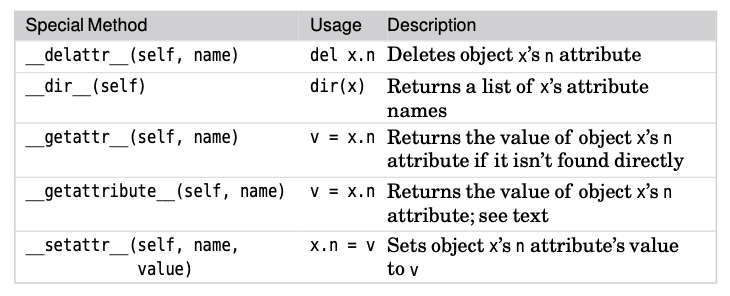
\includegraphics[width=\textwidth]{pics/attribute-special-methods}
  \caption{Attribute access speical methods}
  \label{fig:attribute-special-methods}
\end{figure}





If there are a lot of read-only properites, here is a different solution:
\begin{lstlisting}
USE_GETATTR = True


class Image:
    def __init__(self, width, height, filename="", background="#FFFFFF"):
        self.filename = filename
        self.__background = background
        self.__data = {}
        self.__width = width
        self.__height = height
        self.__colors = {self.__background}

    if USE_GETATTR:
        def __getattr__(self, name):
            if name == 'color':
                return set(self.__colors)
            classname = self.__class__.__name__
            if name in frozenset({'background', 'width', 'height'}):
                # image = Image(10, 10)
                # image.__dict__
                # {'filename': '',
                #  '_Image__background': '#FFFFFF',
                #  '_Image__data': {},
                #  '_Image__width': 10,
                #  '_Image__height': 10,
                #  '_Image__colors': {'#FFFFFF'}}
                return self.__dict__[f'_{classname}__{name}']
            raise AttributeError(f"'{classname}' object has no attribute {name}")
    else:
        @property
        def background(self):
            return self.__background

        @property
        def width(self):
            return self.__width

        @property
        def height(self):
            return self.__height

        @property
        def colors(self):
            return set(self.__colors)
\end{lstlisting}

If the variable \verb|USE_GETATTR| is true, \verb|__getattr__| is used to create read-only properites, otherwise the property decorator is used to create the read-only properties.

If we attemt to access an object's attribute and the attribute is not found, Python will call the \verb|__getattr__| method with the name of the attribute as a parameter.


There is a subtle difference in the that:
\begin{itemize}
\item using \verb|__getattr__()| provides access to the attribute in the instance's class (which may be subclass)
\item accessing the attribute directly uses the class the attribute is defined in 
\end{itemize}



Where as the \verb|__getattr__()| method is called last when looking for (nonspeical) attribute, the \verb|__getattribute__()| method is called first for every attribute access.
Although it can be useful or even essential in some cases to call \verb|__getattribute__()|, reimplementing the \verb|__getattribute__()| method can be tricky.


\subsection{Functors}

In Python, a \keyword{function object} is an object reference to any callable, such as a function, a lambda function, or a method.
The definition also includes classes, since an object reference to a class is a callable that, when called, returns an object of the given class.
In computer science a \keyword{functor} is an object that can be called as though it ware a function, so in Python terms a functor is just another kind of function object.
Any \keyword{class} that has a \verb|__call__()| special method is a functor.



The key benefit that functors offer is that they can maintain some state information.
\begin{lstlisting}
class Strip:
    def __init__(self, characters):
        self.characters = characters

    def __call__(self, string):
        return string.strip(self.characters)
  
strip_punctuation = Strip(',;:.!?')
print(strip_punctuation('Mike Chyson!'))  # Mike Chyson
\end{lstlisting}

We could achieve the same thing using a plain function or lambda, but if we need to store a bit more state or perform more complex processing, a functor is often the right solution.



A functor’s ability to capture state by using a class is very versatile and powerful,but sometimes it is more than we really need.
Another way to capture state is to use a \keyword{closure}.
\keyword{A closure is a function or method that captures some external state.}

\begin{lstlisting}
def make_strip_function(characters):
    def strip_function(string):
        return string.strip(characters)

    return strip_function  

strip_punctuation = make_strip_function(',;:.!?')
print(strip_punctuation('Mike Chyson!'))  # Mike Chyson

\end{lstlisting}

\begin{tcolorbox}
  If the state are complex, you can you a functor, otherwise you can use a plain function or lambda or closure.
\end{tcolorbox}

\subsection{Context manager}

\keyword{Context managers} allow us to simplify code by ensuring that certain operations are performed before and after a particular block of code is executed.
The behavior is achieved because context managers define two special methods, \verb|__enter__()| and \verb|__exit__()|, that Python treats specially in the scope of a \verb|with| statement.
When a context manager is created in a \verb|with| statement its \verb|__enter__()| method is automatically called, and
when the context manager goes out of scope after its with statement its \verb|__exit__()| method is automatically called.


The syntax for using context managers is:
\begin{tcolorbox}
\begin{verbatim}
with expression as variable
    suite
\end{verbatim}
\end{tcolorbox}

The \verb|expression| must be or must produce a context manager object;
if the optional \verb|as variable| part is specified, the variable is set to refer to the object returned by the context manager’s \verb|__enter__()| method (and this is often the context manager itself).
Because a context manager is guaranteed to execute its ``exit'' code (even in the face of exceptions), context managers can be used to eliminate the need for \verb|finally| blocks in many situations.
\keyword{The file objects returned by the built-in open() function are context managers.}


A file object is a context manager whose exit code always closes the file if it was opened.
The exit code is executed whether or not an exception occurs, but in the latter case, the exception is propagated.
This ensures that the file gets closed and we still get the chance to handle any errors.
For example:
\begin{lstlisting}
# without context manager
fh = None
try:
    fh = open(filename)
    for line in fh:
        process(line)
except EnvironmentError as err:
    print(err)
finally:
    if fh is not None:
        fh.close()

# with context manager
try:
    with open(filename) as fh:
        for line in fh:
            process(line)
except EnvironmentError as err:
    print(err)  
\end{lstlisting}

\begin{lstlisting}
try:
    with open(source) as fin, open(target, 'w') as fout:
        for line in fin:
            fout.write(process(line))
except EnvironmentError as err:
    print(err)  
\end{lstlisting}



If we want to create a custom context manager we must create a class that provides two methods: \verb|__enter__()| and \verb|__exit__()|.
Whenever a \verb|with| statement is used on an instance of such a class, the \verb|__enter__()| method is called and the return value is used for the \verb|as variable| (or thrown away if there isn’t one).
When control leaves the scope of the \verb|with| statement the \verb|__exit__()| method is called (with details of an exception if one has occurred passed as arguments).



Suppose we want to perform several operations on a list in an atomic manner.
For example, if we have a list of integers and want to append an integer, delete an integer, and change a couple of integers, all as a single operation, we could write code like this:
\begin{lstlisting}
try:
    with AtomicList(items) as atomic:
        atomic.append(1111)
        del atomic[3]
        atomic[8] = 2222
        atomic[index] = 3333
except (AttributeError, IndexError, ValueError) as err:
    print('no changes applied:', err)  
\end{lstlisting}


Here is the code for the AtomicList context manager:
\begin{lstlisting}
class AtomicList:
    def __init__(self, alist, shallow_copy=True):
        self.original = alist
        self.shallow_copy = shallow_copy

    def __enter__(self):
        self.modified = (self.original[:] if self.shallow_copy else copy.deepcopy(self.original))
        return self.modified

    def __exit__(self, exc_type, exc_val, exc_tb):
        if exc_type is None:  # exception type
            self.original[:] = self.modified  
\end{lstlisting}


If no exception occurred the \verb|exc_type| (``exception type'') will be \verb|None| and we know that we can safely replace the original list’s items with the items from the modified list.
(We cannot do \verb|self.original = self.modified| because that would just replace one object reference with another and would not affect the original list at all.
There is no \verb|return| in \verb|__exit__()|)
But if an exception occurred, we do nothing to the original list and the modified list is discarded.



The return value of \verb|__exit__()| is used to indicate whether any exception that occurred should be propagated.
A \verb|True| value means that we have handled any exception and so no propagation should occur.
Normally we always return \verb|False| or something that evaluates to \verb|False| in a Boolean context to allow any exception that occurred to propagate.
By not giving an explicit \verb|return| value, our \verb|__exit__()| returns \verb|None| which evaluates to \verb|False| and correctly causes any exception to propagate.



\subsection{Descriptors}

Descriptors are \keyword{classes} which provide access control for the attributes of other \keyword{classes}.
Any class that implements one or more of the descriptor special methods, \verb|__get__()|, \verb|__set__()|, and \verb|__delete__()|, is called (and can be used as) a descriptor.


The built-in \verb|property()| and \verb|classmethod()| functions are implemented using descriptors.
The key to understanding descriptors is that although we create an instance of a descriptor in a class as a class attribute, Python accesses the descriptor through the class's instances.



Let’s imagine that we have a class whose instances hold some strings.
We want to access the strings in the normal way, for example, as a property, but we also want to get an XML-escaped version of the strings whenever we want.
One simple solution would be that whenever a string is set we immediately create an XML-escaped copy.
But if we had thousands of strings and only ever read the XML version of a few of them, we would be wasting a lot of processing and memory for nothing.
So we will create a descriptor that will provide XML-escaped strings on demand \keyword{without storing them}.
Here's the client(owner) class, that is, the class uses the discriptor:


\begin{lstlisting}
class Product:
    __slots__ = ('__name', '__description', '__price')

    name_as_xml = XmlShadow('name')
    description_as_xml = XmlShadow('description')

    def __init__(self, name, description, price):
        self.__name = name
        self.__description = description
        self.__price = price

    @property
    def name(self):
        return self.__name

    @property
    def description(self):
        return self.__description

    @description.setter
    def description(self, description):
        self.__description = description

    @property
    def price(self):
        return self.__price

    @price.setter
    def price(self, price):
        self.__price = price

product = Product("Chisel <3cm>", "Chisel & cap", 45.25)
print(product.name, product.name_as_xml, product.description_as_xml, sep='\n')
# Chisel <3cm>
# Chisel &lt;3cm&gt;
# Chisel &amp; cap

\end{lstlisting}

The \verb|name_as_xml| and \verb|description_as_xml| class attributes are set to be instances of the \verb|XmlShadow| descriptor.
Although no \verb|Product| object has a \verb|name_as_xml| attribute or a \verb|description_as_xml| attribute, thanks to the descriptor we can write code like the previous.
This work because when we try to access, for example \verb|name_as_xml| attribute, Python finds that the \verb|Product| class has a descriptor with that name, and so uses the descriptor to get the attribute's value.

\begin{lstlisting}
from xml.sax.saxutils import escape

class XmlShadow:
    def __init__(self, attribute_name):
        self.attribute_name = attribute_name

    def __get__(self, instance, owner=None):
        return escape(getattr(instance, self.attribute_name))
\end{lstlisting}

When the \verb|name_as_xml| or \verb|description_as_xml| attribute is looked up, Python calls the descriptor's \verb|__get__()| method.
The \verb|self| argument is the instance of the descriptor, the \verb|instance| argument is the \verb|Product| instance, and the \verb|owner| argument is the owning class (\verb|Product| in this case).
We use the \verb|getattr()| function to retrieve the relevant attribute from the product (in this case the relevant property), and return an XML-escaped version of it.




If the use case was that only a small proportion of the products were accessed for their XML strings, but the strings were often long and the same ones were frequently accessed, we could use a cache.
\begin{lstlisting}
class CachedXmlShadow:
    def __init__(self, attribute_name):
        self.attribute_name = attribute_name
        self.cache = {}

    def __get__(self, instance, owner=None):
        xml_text = self.cache.get(id(instance))
        if xml_text is not None:
            return xml_text
        return self.cache.setdefault(id(instance), escape(getattr(instance, self.attribute_name)))
\end{lstlisting}

We store the unique identity of the instance as key rather than the instance itself because dictionary keys must be hashable, but we don't want to impose that as a requirement on classes that use the \verb|CachedXmlShadow| descriptor.
The key is necessary because descriptors are created per class rather than per instance.



Here's an example that use a descriptor to store all of an object's attrbute data, with the object not needing to store anything itself.

\begin{lstlisting}
class Point:
    # By setting __slots__ to an empty tuple we ensure that the class cannot store
    # any data attributes at all.
    __slots__ = ()
    x = ExternalStorage('x')
    y = ExternalStorage('y')

    def __init__(self, x=0, y=0):
        self.x = x
        self.y = y  
\end{lstlisting}

By setting \verb|__slots__| to an empty tuple we ensure that the class cannot store any data attributes at all.
When \verb|self.x| is assigned to, Python finds that there is a descriptor with the name ``x'', and so uses the descriptor's \verb|__set__()| method.


\begin{lstlisting}
class ExternalStorage:
    __slots__ = ('attribute_name',)
    __storage = {}  # class attribute

    def __init__(self, attribute_name):
        self.attribute_name = attribute_name

    def __set__(self, instance, value):
        self.__storage[id(instance), self.attribute_name] = value

    def __get__(self, instance, owner):
        if instance is None:
            d = {}
            for k in self.__storage.keys():
                if self.attribute_name in k:
                    d[k] = self.__storage[k]
            return d
        return self.__storage[id(instance), self.attribute_name]


p = Point(3, 4)
print(p.x, p.y)  # 3 4
p = Point(1, 2)
print(p.x, p.y)  # 1 2
print(Point.x, Point.y, Point, sep='\n')
# {(140338432304624, 'x'): 3, (140338432304640, 'x'): 1}
# {(140338432304624, 'y'): 4, (140338432304640, 'y'): 2}
# <class '__main__.Point'>

\end{lstlisting}

Although \verb|__storage| is a class attribute, we can access it as \verb|self.__storage|, because Python will look for it as an instance attribute, and not finding it will then look for it as a class attribute.

The implementation of the \verb|__get__()| special method is slightly more sophisticated than before because we provide a means by which all the attribute values in the ExternalStorage instance itself can be accessed.


We create the \verb|Property| descriptor that mimics the behavior of the built-in \verb|property()| function, at least for setters and getters.
Here's the class that makes use of it:
\begin{lstlisting}
class NameAndExtension:
    def __init__(self, name, extension):
        self.__name = name
        self.extension = extension

    @Property
    def name(self):
        return self.__name

    @Property
    def extension(self):
        return self.__extension

    @extension.setter
    def extension(self, extension):
        self.__extension = extension  
\end{lstlisting}


Here's the \verb|Property| decorator:
\begin{lstlisting}
class Property:
    def __init__(self, getter, setter=None):
        self.__getter = getter
        self.__setter = setter
        self.__name__ = getter.__name__

    def __get__(self, instance, owner=None):
        if instance is None:
            return self
        return self.__getter(instance)

    def __set__(self, instance, value):
        if self.__setter is None:
            raise AttributeError(f"'{self.__name__}' is read-only")
        return self.__setter(instance, value)

    def setter(self, setter):
        self.__setter = setter
        return self.__setter
\end{lstlisting}

The class's initializer takes one or two \keyword{functions} as arguments.
If it is used as a decorator, it will get just the decorated function and this becomes the getter, while the setter is set to \verb|None|.
We use the getter's name as the property's name.
So for each property, we have a getter, possiblely a setter, and a name.

When a property is accessed we return the result of calling the getter function where we have passed the instance as its first parameter.
At first sight, \verb|self.__getter()| looks like a method call, but is is not.
In face, \verb|self.__getter| is an attribute, one that happens to hold an object reference to a method that was passed.
So what happens is that first we retrieve the attribute (\verb|self__getter|), and then we call is as a function \verb|()|.
And because it is called as a function rather than a method we must pass in the relevant \verb|self| object explicitly ourselves.
And in the case of a descriptor the \verb|self| object is called \verb|instance|.

The \verb|setter()| method is called when the interpreter reaches, for example, \verb|@extension.setter|, with the function it decorates as its \verb|setter| argument.
It stores the setter method it has been given (which can now be used in the \verb|__set__()| method), and returns the setter, since decorator should return the function or method they decorate.


\subsection{Class decorators}

Class decorators takes a class object, and should return a class -- normally a modified version of the class they decorate.


\subsubsection{Example:  delegate}

Here's an example without class decorator:
\begin{lstlisting}
_identity = lambda x: x


class SortedList:
    def __init__(self, sequence=None, key=None):
        self.__key = key or _identity
        assert hasattr(self.__key, "__call__")
        if sequence is None:
            self.__list = []
        elif (isinstance(sequence, SortedList) and
              sequence.key == self.__key):
            self.__list = sequence.__list[:]
        else:
            self.__list = sorted(list(sequence), key=self.__key)

    def pop(self, index=-1):
        return self.__list.pop(index)

    def __delitem__(self, index):
        del self.__list[index]

    def __getitem__(self, index):
        return self.__list[index]

    def __setitem__(self, index, value):
        raise TypeError("use add() to insert a value and rely on "
                        "the list to put it in the right place")

    def __iter__(self):
        return iter(self.__list)

    def __reversed__(self):
        return reversed(self.__list)

    def __len__(self):
        return len(self.__list)

    def __str__(self):
        return str(self.__list)
\end{lstlisting}


Here's the decorated version:
\begin{lstlisting}
@delegate("__list", ("pop", "__delitem__", "__getitem__",
                     "__iter__", "__reversed__", "__len__", "__str__"))
class SortedList:

    def __init__(self, sequence=None, key=None):
        self.__key = key or _identity
        assert hasattr(self.__key, "__call__")
        if sequence is None:
            self.__list = []
        elif (isinstance(sequence, SortedList) and
              sequence.key == self.__key):
            self.__list = sequence.__list[:]
        else:
            self.__list = sorted(list(sequence), key=self.__key)
\end{lstlisting}

Here's class decorater:
\begin{lstlisting}
def delegate(attribute_name, method_names):
    def decorator(cls):
        nonlocal attribute_name
        if attribute_name.startswith('__'):
            attribute_name = '_' + cls.__name__ + attribute_name
        for name in method_names:
            setattr(cls, name, eval("lambda self, *a, **kw: "
                                    f"self.{attribute_name}.{name}(*a, **kw)"))
        return cls

    return decorator  
\end{lstlisting}

We could not use a plain decorator because we want to pass arguments to the decorator, so we have instead created a function that takes our arguments and then returns a class decorator.
The decorator itself takes a single argument, a class (just as a function decorator takes a single function or method as its argument).


We must use \verb|nonlocal| so that the nested function uses the \verb|attribute_name| from the outer scope rather than attempting to use one from its own scope.
And we must be able to correct the attribute name if necessary to take account of the name mangling of private attributes.
The decorator’s behavior is quite simple:
It iterates over all the method names that the \verb|delegate()| function has been given, and for each one creates a new method which it sets as an attribute on the class with the given method name.


We have used \verb|eval()| to create each of the delegated methods since it can be used to execute a single statement, and a \verb|lambda| statement produces a method or function.
For example, the code executed to produce the \verb|pop()| method is:
\begin{lstlisting}
lambda self, *a, **kw: self._SortedList__list.pop(*a, **kw)  
\end{lstlisting}


\subsubsection{Example: complete comparisons}


In the following example, only \verb|__lt__()| special method is supplied, and the other comparison method is created by the class decorator.
\begin{lstlisting}
@complete_comparisons
class FuzzyBool:
    def __init__(self, value=0.0):
        self.__value = value if 0.0 <= value <= 1.0 else 0.0

    def __lt__(self, other):
        return self.__value < other.__value
\end{lstlisting}


Here's the decorator:
\begin{lstlisting}
def complete_comparisons(cls):
    assert cls.__lt__ is not object.__lt__, (
        f'{cls.__name__} must define < and ideally =='
    )
    if cls.__eq__ is object.__eq__:
        cls.__eq__ = lambda self, other: (
            not (cls.__lt__(self, other) or cls.__lt__(other, self))
        )
    cls.__ne__ = lambda self, other: not cls.__eq__(self, other)
    cls.__gt__ = lambda self, other: cls.__lt__(other, self)
    cls.__le__ = lambda self, other: not cls.__lt__(other, self)
    cls.__ge__ = lambda self, other: not cls.__lt__(self, other)
\end{lstlisting}


Given a class that defines only < (or < and ==), the decorator produces the missing comparison operators by using the following logical equivalences:
\begin{figure}[H]
  \centering
  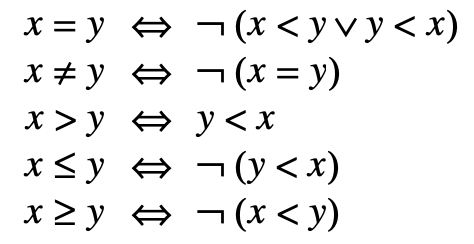
\includegraphics[width=\textwidth]{pics/logical-equivalences}
  \caption{Logical equivalences}
\end{figure}


In fact, Python automatically produces > if < is supplied, != if == is supplied, and >= if <= is supplied, so it is sufficient to just implement the three operators <, <=, and == and to leave Python to infer the others.
However, using the class decorator reduces the minimum that we must implement to just <.
This is convenient, and also ensures that all the comparison operators use the same consistent logic.


One problem that the decorator faces is that class \verb|object| from which every other class is ultimately derived defines all six comparison operators, all of which raise a \verb|TypeError| exception if used.
So we need to know whether < and == have been reimplemented (and are therefore usable).
This can easily be done by comparing the relevant special methods in the class being decorated with those in \verb|object|.



\begin{tcolorbox}
  Using class decorators is probably the simplest and most direct way of changing classes. Another approach is to use metaclasses.
\end{tcolorbox}



\subsection{Abstract base classes}

An abstract base class (ABC) is a class that \keyword{cannot be used to create objects}.
Instead, the purpose of such classes is \keyword{to define interface}, that is, to in effect list the methods and properites that classes that inherit the abstract base class must provide.
This is useful because we can use an abstract base class as a kind of \keyword{promise} -- a promise that any derived class will provide the methods and properites that the abstract base class specifies.


\begin{tcolorbox}
  Abstract base classes are classes that have at least one abstract method or property.
\end{tcolorbox}

\begin{tcolorbox}
  All ABCs must have a metaclass of \verb|abc.ABCMeta| (from the \verb|abc| module), or from one of its subclasses.
\end{tcolorbox}





\subsubsection{Example:  Appliance}

\begin{lstlisting}
import abc


class Appliance(metaclass=abc.ABCMeta):
    @abc.abstractmethod
    def __init__(self, model, price):
        self.__model = model
        self.price = price

    def get_price(self):
        return self.__price

    def set_price(self, price):
        self.__price = price

    price = abc.abstractproperty(get_price, set_price)

    @property
    def model(self):
        return self.__model  
\end{lstlisting}


We have set the class’s metaclass to be \verb|abc.ABCMeta| since this is a requirement for ABCs.
We have made \verb|__init__()| an abstract method to ensure that it is reimplemented, and we have also provided an implementation which we expect (but can’t force) inheritors to call. 
To make an abstract readable/writable property we cannot use decorator syntax; also we have not used private names for the getter and setter since doing so would be inconvenient for subclasses.


The \verb|price| property is abstract (so we cannot use the \verb|@property| decorator), and is readable/wriable data as a property.
We initialize the \keyword{property} in the \verb|__init__()| method rather than setting the private data directly --
this ensures that the setter is called (and may potentially do validation or other work, although it doesn’t in this particular example).



The \verb|model| property is not abstract, so subclasses don’t need to reimplement it, and we can make it a property using the \verb|@property| decorator.



Here is an example subclass:
\begin{lstlisting}
class Cooker(Appliance):
    def __init__(self, model, price, fuel):
        super().__init__(model, price)
        self.fuel = fuel

    price = property(lambda self: super().price,
                     lambda self, price: super().set_price(price))  
\end{lstlisting}


\subsubsection{Example: TextFilter}

\begin{lstlisting}
import abc


class TextFilter(metaclass=abc.ABCMeta):
    @abc.abstractmethod
    def is_tranformer(self):
        raise NotImplementedError()

    @abc.abstractmethod
    def __call__(self):
        raise NotImplementedError()  
\end{lstlisting}

The \verb|TextFilter| ABC provides no functionality at all; it exists purely to define an interface.
Since the abstract property and method have no implementations we don’t want subclasses to call them, so instead of using an innocuous pass statement we raise an exception if they are used



Here are some subclasses:
\begin{lstlisting}
class CharCounter(TextFilter):
    @property
    def is_tranformer(self):
        return False

    def __call__(self, text, chars):
        count = 0
        for c in text:
            if c in chars:
                count += 1
        return count


class RunLengthEncoder(TextFilter):
    @property
    def is_tranformer(self):
        return True

    def __call__(self, utf8_string):
        byte = None
        count = 0
        binary = bytearray()
        for b in utf8_string.encode("utf8"):
            if byte is None:
                if b == 0:
                    binary.extend((0, 1, 0))
                else:
                    byte = b
                    count = 1
            else:
                if byte == b:
                    count += 1
                    if count == 255:
                        binary.extend((0, count, b))
                        byte = None
                        count = 0
                else:
                    if count == 1:
                        binary.append(byte)
                    elif count == 2:
                        binary.extend((byte, byte))
                    elif count > 2:
                        binary.extend((0, count, byte))
                    if b == 0:
                        binary.extend((0, 1, 0))
                        byte = None
                        count = 0
                    else:
                        byte = b
                        count = 1
        if count == 1:
            binary.append(byte)
        elif count == 2:
            binary.extend((byte, byte))
        elif count > 2:
            binary.extend((0, count, byte))
        return bytes(binary)


class RunLengthDecoder(TextFilter):
    @property
    def is_tranformer(self):
        return True

    def __call__(self, rle_bytes):
        binary = bytearray()
        length = None
        for b in rle_bytes:
            if length == 0:
                length = b
            elif length is not None:
                binary.extend([b for x in range(length)])
                length = None
            elif b == 0:
                length = 0
            else:
                binary.append(b)
                length = None
        if length:
            binary.extend([b for x in range(length)])
        return binary.decode("utf8")


if __name__ == '__main__':
    vowel_counter = CharCounter()
    count = vowel_counter('dog fish and cat fish', 'aeiou')
    print(count)  # 5

    print('=' * 100)
    text = 'Mack Chyson ======================='
    encoder = RunLengthEncoder()
    encoded_text = encoder(text)
    print(encoded_text)  # b'Mack Chyson \x00\x17='
    decoder = RunLengthDecoder()
    original_text = decoder(encoded_text)
    print(original_text)
    # Mack Chyson =======================
\end{lstlisting}


\subsubsection{Example: Abstract}

\begin{lstlisting}
class Undo(metaclass=abc.ABCMeta):
    @abc.abstractmethod
    def __init__(self):
        self.__undos = []

    @abc.abstractmethod
    def can_undo(self):
        return bool(self.__undos)

    @abc.abstractmethod
    def undo(self):
        assert self.__undos, 'nothing left to undo'
        self.__undos.pop()(self)

    def add_undo(self, undo):
        self.__undos.append(undo)

    def clear(self):
        self.__undos = []  
\end{lstlisting}

The \verb|self.__undos| list is exprected to hold object references to methods.
Each method must cause the corresponding action to be undone if it is called.
So to perform an undo we pop the last undo method off the \verb|self.__undos| list, and then call the method as a function, passing \verb|self| as an argument.
(We must pass \verb|self| because the method is being called as a function not at a method.)


Here's \verb|Stack| class:
\begin{lstlisting}
class Stack(Undo):
    def __init__(self):
        super().__init__()
        self.__stack = []

    @property
    def can_undo(self):
        return super().can_undo

    def undo(self):
        super().undo()

    def push(self, item):
        self.__stack.append(item)
        self.add_undo(lambda self: self.__stack.pop())

    def pop(self):
        item = self.__stack.pop()
        self.add_undo(lambda self: self.__stack.append(item))
        return item

    def top(self):
        assert self.__stack, 'Stack is empty'
        return self.__stack[-1]

    def __str__(self):
        return str(self.__stack)
\end{lstlisting}


\subsection{Multiple inheritance}

Multiple inheritance is where one class inherits from two or more other classes.
One problem is that multiple inheritance can lead to the same class being inherited more than once and this means that the version of a method that is called depends on the method resolution order,
which potentially makes classes that use multiple inheritance somewhat fragile.



Multiple inheritance can generally ba avoided by:
\begin{itemize}
\item Using single inheritance and setting a metaclass if we want to support an additional API
\item Using mutiple inheritance with one concrete class and one or more abstract base classes for addtional APIs
\item Using single inheritance and aggregate instances of other classes
\end{itemize}





Nonetheless, in some cases, multiple inheritance can provide a very convenient solution.
For example, suppose we want to create a new version of the \verb|Stack| class from the previous subsection, but want the class to support loading and saving using a pickle.
We might well want to add the loading and saving functionality to several classes, so we will implement it in a class of its own:
\begin{lstlisting}
class LoadSave:
    def __init__(self, filename, *attribute_names):
        self.filename = filename
        self.__attribute_names = []
        for name in attribute_names:
            if name.startswith('__'):
                name = '_' + self.__class__.__name__ + name
            self.__attribute_names.append(name)

    def save(self):
        with open(self.filename, 'wb') as fh:
            data = []
            for name in self.__attribute_names:
                data.append(getattr(self, name))
            pickle.dump(data, fh, pickle.HIGHEST_PROTOCOL)

    def load(self):
        with open(self.filename, 'rb') as fh:
            data = pickle.load(fh)
            for name, value in zip(self.__attribute_names, data):
                setattr(self, name, value)
  
\end{lstlisting}


\begin{lstlisting}
class FileStack(Undo, LoadSave):
    def __init__(self, filename):
        Undo.__init__(self)
        LoadSave.__init__(self, filename, '__stack')
        self.__stack = []

    def load(self):
        super().load()
        Undo.clear(self)
\end{lstlisting}

Instead of using \verb|super()| in the \verb|__init__()| method we must specify the base classes that we initialize since \verb|super()| cannot guess out intensions.


\begin{tcolorbox}
  Multiple inheritance can be convenient and works well when the inheritance classes have no overlapping APIs.
\end{tcolorbox}



\subsection{Metaclasses}

A metaclass is to a class what a class is to an instance; that is, a metaclass is used to create classes, just as classes are used to create instances.
We can ask whether a class object inherits another class using \verb|issubclass()|.


\subsubsection{Register}


The simplest use of metaclasses is to make custom classes fit into Python's standard ABC hierarchy.

\begin{lstlisting}
import collections


class SortedList:
    pass


collections.abc.Sequence.register(SortedList)
\end{lstlisting}


Registering a class like this makes it a \keyword{virtual subclass}.
A virtual subclass reports that it is a subclass of the class or classes it it registed with, but does not inherit any data or methods from any of the classes it is registered with.
Registering a class like this provides a promise that the class provides the API of the classes it is registered with, but does not provide any guarantee that it will honor its promise.


\subsubsection{Guarantee}


One use of metaclasses is to provide both a promise and a guarantee about a class's API.
Another use is to modify a class in some way (like a class decorator does).
And metaclasses can be used for both purposes at the same time.



Suppose we want to create a group of classes that all provide \verb|load()| and \verb|save()| methods.
We can do this by creating a class that when used as a metaclass, checks that these methods are present:

\begin{lstlisting}
# API guarantee
class LoadableSavable(type):
    def __init__(cls, classname, bases, dictionary):
        super().__init__(classname, bases, dictionary)

        assert (
            hasattr(cls, 'load') and
            isinstance(getattr(cls, 'load')), collections.abc.Callable
        ), "class '" + classname + "' must provide a load() method"
        assert (
                hasattr(cls, 'save') and
                isinstance(getattr(cls, 'save'), collections.abc.Callable)
        ), "class '" + classname + "' must provide a save() method"
\end{lstlisting}



Classes that are to serve as metaclasses must inherit from the ultimate metaclass base class, \verb|type|, or one of its subclasses.


Once the class has been created, the metaclass is initialized by calling its \verb|__init__()| method.
The arguments given to \verb|__init__()| are \verb|cls|, the class that just been created;
\verb|classname|, the class's name;
\verb|bases|, a list of the class's base classes (excluding \verb|object|, and therefore possibly empty);
and \verb|dictionary| that holds the attributes that became class attributes when the \verb|cls| class was created,
unless we intervened in a reimplementation of the metaclass's \verb|__new__()| method.



\begin{lstlisting}
# class Bad(metaclass=LoadableSavable):
#     def some_method(self): pass
# AssertionError: class 'Bad' must provide a load() method

class Good(metaclass=LoadableSavable):
    def load(self): pass
    def save(self): pass


g = Good()
\end{lstlisting}



\subsubsection{Modify}

We can use metaclasses to change the classes use them.
If the change involves the name, base classes, or dictionary of the class being created, the we need to reimplement the metaclass's \verb|__new__()| method;
buf for other changes, such as adding methods or data attributes, reimplementing \verb|__init__()| is sufficient, although this can also be done in \verb|__new__()|.





This exmaple is just used to show the modification function.
Normall the following code is not good.
Suppose we did not use property decorators before, but use a simple naming convetion ti identify properties.
Here, the class has methods of the form \verb|get_name()| and \verb|set_name()|, we would expect the class to have a private \verb|__name| property accessed using \verb|instance.name| for getting and setting.
Here is the class:

\begin{lstlisting}
class Product(metaclass=AutoSlotProperties):
    def __init__(self, barcode, description):
        self.__barcode = barcode
        self.description = description

    def get_barcode(self):
        return self.__barcode

    def get_description(self):
        return self.__description

    def set_description(self, description):
        if description is None or len(description) < 3:
            self.__description = '<Invalid Description>'
        else:
            self.__description = description
\end{lstlisting}

This can be done using a metaclass.

\begin{lstlisting}
# modifying properties
class AutoSlotProperties(type):
    def __new__(mcl, classname, bases, dictionary):
        slots = list(dictionary.get('__slot__', []))  # get slots
        for getter_name in [key for key in dictionary if key.startswith('get_')]:
            if isinstance(dictionary[getter_name], collections.abc.Callable):
                name = getter_name[4:]
                slots.append('__' + name)  # alter slots
                getter = dictionary.pop(getter_name)
                setter_name = 'set_' + name
                setter = dictionary.get(setter_name, None)
                if setter is not None and isinstance(setter, collections.abc.Callable):
                    del dictionary[setter_name]
                dictionary[name] = property(getter, setter)  # convert to property
        dictionary['__slots__'] = tuple(slots)
        return super().__new__(mcl, classname, bases, dictionary)  



product = Product('111', '8mm Stapler')
print(product.barcode, product.description)  # 111 8mm Stapler
product.description = '8mm Stapler (long)'
print(product.barcode, product.description)  # 111 8mm Stapler (long)

print(product.__slots__)  # ('__barcode', '__description')

for i in dir(product):
    print(i)
# _Product__barcode
# _Product__description
# __class__
# __delattr__
# __dir__
# __doc__
# __eq__
# __format__
# __ge__
# __getattribute__
# __gt__
# __hash__
# __init__
# __init_subclass__
# __le__
# __lt__
# __module__
# __ne__
# __new__
# __reduce__
# __reduce_ex__
# __repr__
# __setattr__
# __sizeof__
# __slots__
# __str__
# __subclasshook__
# barcode
# description  
\end{lstlisting}



\section{Functional-style programming}


Functional-style programming is an approach to programming where computations are built up from combining functions:
\begin{itemize}
\item tha don't modify their arguments and 
\item that don't refer to or change the program's state, and 
\item that provide their results as return values.
\end{itemize}



Three concepts that are strongly associated with functional programming are
\begin{enumerate}
\item mapping
\item filtering
\item reducing
\end{enumerate}


Mapping involves taking a function and an iterable and producing a new iterable (or a list) where each item is the result of calling the function on the corresponding item in the original iterable.
This is supported by the built-in \verb|map()| function, for example:
\begin{lstlisting}
list(map(lambda x: x ** 2, [1, 2, 3, 4]))
Out[3]: [1, 4, 9, 16]  
\end{lstlisting}



Filtering involves taking a function and an iterable and producing a new iterable where each item is from the original iterable -- providing the function returns True when called on the item.
The built-in \verb|filter()| function supports this:
\begin{lstlisting}
list(filter(lambda x: x > 0, [1, -2, 3, -4]))
Out[5]: [1, 3]  
\end{lstlisting}


Reducing involves taking a function and an iterable and producing a single result value.
The way this works is that the function is called on the iterable’s first two values, then on the computed result and the third value, then on the computed result and the fourth value, and so on, until all the values have been used. 
The \verb|functools| module's \verb|functools.reduce()| function supports this.
\begin{lstlisting}
import functools
functools.reduce(lambda x, y: x * y, [1, 2, 3, 4])
Out[7]: 24
import operator
functools.reduce(operator.mul, [1, 2, 3, 4])
Out[9]: 24
\end{lstlisting}


The \verb|operator| module has functions for all of Python’s operators specifically to make functional-style programming easier. 





Python provides some built-in reducing functions:
\begin{description}
\item[all()] given an iterable, returns \verb|True| if all the iterable’s items return \verb|True| when \verb|bool()| is applied to them;
\item[any()] returns \verb|True| if any of the iterable’s items is \verb|True|;
\item[max()] returns the largest item in the iterable;
\item[min()] returns the smallest item in the iterable; 
\item[sum()] returns the sum of the iterable’s items.
\end{description}




\subsection{Partial function application}

Partial function application is the creation of a function from an existing function and some arguments to produce a new function that does what the original function did, but with some arguments fixed so that callers don’t have to pass them.
Here’s a very simple example:
\begin{lstlisting}
enumerate1 = functools.partial(enumerate, start=1)
for lino, line in enumerate1(lines):
    process_line(lino, line)
\end{lstlisting}



Using partial function application can simplify our code, especially when we want to call the same functions with the same arguments again and again.
For example:

\begin{lstlisting}
reader = functools.partial(open, mode='rt', encoding='utf8')
writer = functools.partial(open, mode='wt', encoding='utf8')
\end{lstlisting}

\begin{lstlisting}
Conv2D_ = functools.partial(Conv2D, kernel_size=(3, 3), activation='relu', padding='same')

h = Conv2D_(256)(input_layer)
h = Conv2D_(64)(h)

# The same full code is:
# h = Conv2D(256, (3, 3), activation='relu', padding='same')(input_layer)
# h = Conv2D(64, (3, 3), activation='relu', padding='same')(h)  
\end{lstlisting}


\subsection{Coroutines}

Coroutines are functions whose processing can be suspended and resumed at specific points.


In Python, a coroutine is a function that takes its input from a \verb|yield| expression.
It may also send results to a receiver function (which itself must be a coroutine).
Whenever a coroutine reaches a \verb|yield| expression it suspends waiting for data; and once it receives data, it resumes execution from that point.


\subsubsection{Composing pipelines}

A pipeline is simply the composition of one or more functions where data items are sent to the first function, which then either discards the item (filters it out) or passes it on to the next function (either as is or transformed in some way).
The second function receives the item from the first function and repeats the process, discarding or passing on the item (possibly transformed in a different way) to the next function, and so on.
Items that reach the end are then output in some way.


\begin{tcolorbox}
One benefit of using pipelines is that we can read data items incrementally, often one at a time, and have to give the pipeline only enough data items to fill it (usually one or a few items per component).
This can lead to significant \keyword{memory savings} compared with, say, reading an entire data set into memory and then processing it all in one go.  
\end{tcolorbox}



Here is an example -- a file matcher that reads all the filenames given on the command line (including those in the directories given on the command line, recursively), and that output the absolute paths of those files that meet certain criteria.




\begin{lstlisting}
import os
import sys
import functools


def coroutine(function):
    @functools.wraps(function)
    def wrapper(*args, **kwargs):
        generator = function(*args, **kwargs)
        next(generator)
        return generator

    return wrapper


@coroutine
def reporter():
    while True:
        filename = (yield)
        print(filename)


@coroutine
def get_files(receiver):
    """
    A wrapper of os.walk()
    :param receiver:
    :return:
    """
    while True:
        path = (yield)
        if os.path.isfile(path):
            receiver.send(os.path.abspath(path))
        else:
            for root, dirs, files in os.walk(path):
                for filename in files:
                    receiver.send(os.path.abspath(os.path.join(root, filename)))


@coroutine
def suffix_matcher(receiver, suffixes):
    while True:
        filename = (yield)
        if filename.endswith(suffixes):
            receiver.send(filename)


@coroutine
def size_matcher(receiver, minimum=None, maximum=None):
    while True:
        filename = (yield)
        size = os.path.getsize(filename)
        if ((minimum is None or size >= minimum) and
                (maximum is None or size <= maximum)):
            receiver.send(filename)


if __name__ == '__main__':
    # notice the order in coroutine
    pipes = []
    pipes.append(reporter)
    pipes.append(size_matcher(pipes[-1], minimum=1024))
    pipes.append(suffix_matcher(pipes[-1], (".png", ".jpg", ".jpeg", ".py")))
    pipes.append(get_files(pipes[-1]))
    pipeline = pipes[-1]
    # Equal to
    # pipeline = get_files(suffix_matcher(size_matcher(reporter(), minimum=1024), (".png", ".jpg", ".jpeg", ".py")))

    try:
        for file in sys.argv[1:]:
            print(file)
            pipeline.send(file)
            # pipeline.py
            # /Users/mike/PycharmProjects/python3/c8_advanced_programming_techniques/functional_programming/pipeline.py
            # partial.py
            # /Users/mike/PycharmProjects/python3/c8_advanced_programming_techniques/functional_programming/partial.py
            # __init__.py
    finally:
        for pipe in pipes:
            pipe.close()
  
\end{lstlisting}

The \verb|@coroutine| decorator takes a coroutine function, and calls the built-in \verb|next()| function on it -- this causes the function to be executed up to the first \verb|yield| expression, ready to receive data.






\chapter{Debugging, testing, and profiling}

Writing programs is a mixture of art, craft, and science, and because it is done by \keyword{humans}, mistakes are made.


Mistackes fall into sevaral categories:
\begin{description}
\item[syntax error] The program can not run.
\item[logical error] The program runs, but some aspect of its behavior is not what we intended or expected.
\item[poor performance] This is almost always due to a poor choice of algorithm or data structure or both.
\end{description}

\section{Debugging}


\subsection{Dealing with syntax errors}

\begin{lstlisting}
for i in range(10)
    print(1)

#   File "/Users/mike/PycharmProjects/python3/c9_debugging_testing_profiling/t.py", line 10
#     for i in range(10)
#                      ^
# SyntaxError: invalid syntax  
\end{lstlisting}

If we try to run a program that has a syntax error, Python will stop execution and print the filename, line number, and offending line, with a caret(\^{}) underneath indicating exactly where the error was detected.


\begin{lstlisting}
try:
    if True:
        print(''
except Exception as err:
    print(err)
    
#   File "/Users/mike/PycharmProjects/python3/c9_debugging_testing_profiling/t.py", line 21
#     except Exception as err:
#     ^
# SyntaxError: invalid syntax  
\end{lstlisting}

There is no syntax error in the line indicated, so both the line number and the caret’s position are wrong.
We have omite a parenthese, but Python didn't realize this until it reach the \verb|except| keyword on the following line.




\subsection{Dealing with runtime errors}

\begin{lstlisting}
def div():
    1 / 0


if __name__ == '__main__':
    div()

# Traceback (most recent call last):
#   File "/Users/mike/PycharmProjects/python3/c9_debugging_testing_profiling/e3.py", line 17, in <module>
#     div()
#   File "/Users/mike/PycharmProjects/python3/c9_debugging_testing_profiling/e3.py", line 13, in div
#     1 / 0
# ZeroDivisionError: division by zero  
\end{lstlisting}

If an unhandled exception occurs at runtime, Python will stop executing our program and print a traceback.
Tracebacks should be read from their last line back toward their first line.
The last line specifies the unhandled exception that occurred.
Above the line, the filename, line number, and function name, followed by the line that caused the exception, are shown.


\subsection{Scientific debugging}

To be able to kill a bug we must be able to do the following.
\begin{enumerate}
\item Reproduce the bug.
\item Locate the bug.
\item Fix the bug.
\item Test the fix.
\end{enumerate}


Reproducing the bug is sometimes easy -- it always occurs on every run; and sometimes hard -- it occurs intermittently.
In either case we should try to reduce the bug’s dependencies, that is, find the smallest input and the least amount of processing that can still produce the bug.


The scientific method of finding and fixing the bug has three steps:
\begin{enumerate}
\item Think up an explanation -- a hypothesis -- that reasonably accounts for the bug.
\item Create an experiment to test the hypothesis.
\item Run the experiment.
\end{enumerate}


\section{Unit testing}

A key point of TDD (Test Driven Development) is that when we want to add a feature, we \keyword{frist} write a test for it.


Python's standard library provides two unit testing modules, \verb|doctest| and \verb|unittest|.
Creating doctests is straightforward:
We write the tests in the module, function, class, and methods’ docstrings, and for modules, we simply add three lines at the end of the module:
\begin{lstlisting}
if __name__ == "__main__":
    import doctest
    doctest.testmod()
\end{lstlisting}

To exercise the program's doctests there there are two approaches:
\begin{enumerate}
\item Import the \verb|doctest| module and then run the program -- for example, at the console, \verb|python -m doctest yourprogram.py|.
\item Create a separate test program using the \verb|unittest| module.
\end{enumerate}




\section{Profiling}

There are some programming habits that are good for performance:
\begin{itemize}
\item Prefer tuples to lists when read-only sequence is needed.
\item Use generators rather than creating large tuples or lists to iterate over.
\item Use Python’s built-in data structures -- \verb|dicts|, \verb|lists|, and \verb|tuples| -- rather than custom data structures implemented in Python, since the built-in ones are all very highly optimized.
\item When creating large strings out of lots of small strings, instead of concatenating the small strings, accumulate them all in a list, and join the list of strings into a single string at the end.
\item If an object (including a function or method) is accessed a large number of times using attribute access (e.g., when accessing a function in a module), or from a data structure, it may be better to create and use a local variable that refers to the object to provide faster access.
\end{itemize}




The \verb|cProfile| module (or the \verb|profile| module) can be sued to compare the performance of functions and methods.
And it also shows precisely what is being called and how long each call takes.


\begin{lstlisting}
import cProfile
import math


def log(x, y):
    return math.log(x, y)


code = """
for i in range(10000):
    log(10, 2)
"""
cProfile.run(code)
\end{lstlisting}


\begin{verbatim}
         20003 function calls in 0.006 seconds

   Ordered by: standard name

   ncalls  tottime  percall  cumtime  percall filename:lineno(function)
        1    0.002    0.002    0.006    0.006 <string>:2(<module>)
    10000    0.002    0.000    0.004    0.000 cprofile_.py:5(log)
        1    0.000    0.000    0.006    0.006 {built-in method builtins.exec}
    10000    0.002    0.000    0.002    0.000 {built-in method math.log}
        1    0.000    0.000    0.000    0.000 {method 'disable' of '_lsprof.Profiler' objects}
\end{verbatim}

The \verb|ncalls| (``number of calls'') column lists the number of calls to the specified function.
The \verb|tottime| (``total time'') column lists the total time spent in the function, but excluding time spent inside functions called by the function.
The first \verb|percall| column lists the average time of each all to the function (\verb|tottime| // \verb|ncalls|).
The \verb|cumtime| (``cumulative time'') column lists the time spent in the function and includes the time spent inside functions called by the function.
The second \verb|percall| column lists the average time of each call to the function, including functions called by it.




The \verb|cProfile| module allows us to profile code without instrumenting it.
The command line to use is \verb|python -m cProfile program_or_module.py|.

\verb|MyModule.py|:
\begin{lstlisting}
import math


def log(x, y):
    return math.log(x, y)


for i in range(10000):
    log(10, 2)
  
\end{lstlisting}

We can save the complement profile data and analyze it using the \verb|pstats| module.

\begin{lstlisting}

(base) mike@Mikes-MacBook-Pro c9_debugging_testing_profiling % python -m cProfile -o profile.dat MyModule.py
(base) mike@Mikes-MacBook-Pro c9_debugging_testing_profiling % python -m pstats                             
Welcome to the profile statistics browser.
% read profile.dat
profile.dat% callers log
   Random listing order was used
   List reduced from 65 to 2 due to restriction <'log'>

Function                    was called by...
                                ncalls  tottime  cumtime
{built-in method math.log}  <-   10000    0.001    0.001  MyModule.py:4(log)
MyModule.py:4(log)          <-   10000    0.002    0.003  MyModule.py:1(<module>)


profile.dat% callees log
   Random listing order was used
   List reduced from 65 to 2 due to restriction <'log'>

Function                    called...
                                ncalls  tottime  cumtime
{built-in method math.log}  -> 
MyModule.py:4(log)          ->   10000    0.001    0.001  {built-in method math.log}


profile.dat% quit
Goodbye.
  
\end{lstlisting}



\chapter{Processes and threading}

With the advant of \keyword{multicore} processors, it is more tempting and more practical than ever before to spread the processing load so as to get the most out of all the avaiable cores.
There are two main approaches to spreading the workload:
\begin{itemize}
\item multiple processes
\item multiple threads
\end{itemize}



\begin{table}[htb!]
  \centering
  \begin{tabular}{p{0.3\columnwidth}p{0.3\columnwidth}p{0.3\columnwidth}}
    \toprule{}
    & \head{advantage} & \head{disadvantage} \\
    \midrule
    multiple processes & each process runs independently & communication and data sharing can be inconvenient \\
    multiple threads & can communicate simply by data sharing & more complex than single-threaded program\\
    \bottomrule
  \end{tabular}
  \caption{multiple processes and multiple threads}
\end{table}


\section{Using the multiprocessing module}

\begin{lstlisting}
#!/usr/bin/env python3
"""
@project: python3
@file: grepword_p
@author: mike
@time: 2021/2/22

@function:
Searches for a word specified on the command line in the files listed after the word.
This the parent program. 
The corresponding child program is grepword_p_child.py.
"""
import os
import sys
import subprocess
import optparse


def main():
    child = os.path.join(os.path.dirname(__file__), 'grepword_p_child.py')
    opts, word, args = parse_options()
    filelist = get_files(args, opts.recurse)
    files_per_process = len(filelist) // opts.count
    # Usually the number of files won’t be an exact multiple of the number of processes,
    # so we increase the number of files the first process is given by the remainder.
    start, end = 0, files_per_process + (len(filelist) % opts.count)
    number = 1

    pipes = []
    while start < len(filelist):
        command = [sys.executable, child]
        if opts.debug:
            command.append(str(number))
        pipe = subprocess.Popen(command, stdin=subprocess.PIPE)
        pipes.append(pipe)
        pipe.stdin.write(word.encode('utf8') + b'\n')
        for filename in filelist[start:end]:
            pipe.stdin.write(filename.encode('utf8') + b'\n')
        pipe.stdin.close()
        number += 1
        start, end = end, end + files_per_process

    while pipes:
        pipe = pipes.pop()
        pipe.wait()


def parse_options():
    parser = optparse.OptionParser(
        usage=("usage: %prog [options] word name1 "
               "[name2 [... nameN]]\n\n"
               "names are filenames or paths; paths only "
               "make sense with the -r option set"))
    parser.add_option("-p", "--processes", dest="count", default=7,
                      type="int",
                      help=("the number of child processes to use (1..20) "
                            "[default %default]"))
    parser.add_option("-r", "--recurse", dest="recurse",
                      default=False, action="store_true",
                      help="recurse into subdirectories")
    parser.add_option("-d", "--debug", dest="debug", default=False,
                      action="store_true")
    opts, args = parser.parse_args()
    if len(args) == 0:
        parser.error("a word and at least one path must be specified")
    elif len(args) == 1:
        parser.error("at least one path must be specified")
    if (not opts.recurse and
            not any([os.path.isfile(arg) for arg in args])):
        parser.error("at least one file must be specified; or use -r")
    if not (1 <= opts.count <= 20):
        parser.error("process count must be 1..20")
    return opts, args[0], args[1:]


def get_files(args, recurse):
    filelist = []
    for path in args:
        if os.path.isfile(path):
            filelist.append(path)
        elif recurse:
            for root, dirs, files in os.walk(path):
                for filename in files:
                    filelist.append(os.path.join(root, filename))
    return filelist


main()  
\end{lstlisting}


The \verb|number| variable (line 22) is used purely for debugging so that we can see which process produce each line of output.
For each \verb|start:end| slice of the \verb|filelist| we specify the Python interpreter (conveniently available in \verb|sys.executable|) (line 26).

Once all the processes have started we wait for each child process to finish.
This is not essential, but on Unix-like systems it ensures that we are returned to the console prompt when all the processes are done (otherwise, we must press Enter when they are all finished).
Another benefit of waiting is that if we interrupt the program (e.g., by pressing Ctrl+C), all the processes that are still running will be interrupted and will terminate with an uncaught \verb|KeyboardInterrupt| exception --
if we did not wait the main program would finish (and therefore not be interruptible), and the child processes would continue (unless killed by a kill program or a task manager).




\begin{lstlisting}
#!/usr/bin/env python3
"""
@project: python3
@file: grepword_p_child
@author: mike
@time: 2021/2/22
 
@function:
"""
import sys

coding = 'utf8'
BLOCK_SIZE = 8000
number = f'{sys.argv[1]}' if len(sys.argv) == 2 else ''
stdin = sys.stdin.buffer.read()
lines = stdin.decode(coding, 'ignore').splitlines()
word = lines[0].rstrip()

for filename in lines[1:]:
    filename = filename.rstrip()
    previous = ''
    try:
        with open(filename, 'rb') as fh:
            while True:
                current = fh.read(BLOCK_SIZE)
                if not current:
                    break
                current = current.decode(coding, 'ignore')
                if word in current or word in previous[-len(word):] + current[:len(word)]:
                    print(f'{number}{filename}')
                    break
                if len(current) != BLOCK_SIZE:
                    break
                previous = current
    except EnvironmentError as err:
        print(f'{number}{err}')
  
\end{lstlisting}

It is possible that some of the files might be very large and this could be a problem, especially if there are 20 child processes running concurrently, all reading big files.
We handle this by reading each file in blocks, keeping the previous block read to ensure that we don’t miss cases when the only occurrence of the search word happens to fall across two blocks.


\section{Using the threading module}

Setting up two or more separate threads of execution in Python is quite straightforward.
The complexity arises when we want to separate threads to share data.

One common solution is to use some kind of locking mechanism.



Every Python program has at least one thread, the main thread.
To create multiple threads we must import the \verb|threading| module and use that to create as many additional threads as want.
There are two ways to create threads:
\begin{enumerate}
\item We can call \verb|threading.Thread()| and pass it a callable object
\item We can subclass the \verb|threading.Thread| class.
\end{enumerate}



\begin{lstlisting}
#!/usr/bin/env python3
"""
@project: python3
@file: grepword_t
@author: mike
@time: 2021/2/22
 
@function:
"""

import queue
import os
import threading

BLOCK_SIZE = 8000
from grepword_p import parse_options, get_files


def main():
    opts, word, args = parse_options()
    filelist = get_files(args, opts.recurse)
    work_queue = queue.Queue()
    for i in range(opts.count):
        number = f'{i + 1}: ' if opts.debug else ''
        worker = Worker(work_queue, word, number)
        worker.daemon = True
        worker.start()
    for filename in filelist:
        work_queue.put(filename)
    work_queue.join()


class Worker(threading.Thread):
    def __init__(self, work_queue, word, number):
        super().__init__()
        self.work_queue = work_queue
        self.word = word
        self.number = number

    def run(self) -> None:
        while True:
            try:
                filename = self.work_queue.get()
                self.process(filename)
            finally:
                self.work_queue.task_done()

    def process(self, filename):
        previous = ""
        try:
            with open(filename, "rb") as fh:
                while True:
                    current = fh.read(BLOCK_SIZE)
                    if not current:
                        break
                    current = current.decode("utf8", "ignore")
                    if (self.word in current or
                            self.word in previous[-len(self.word):] +
                            current[:len(self.word)]):
                        print("{0}{1}".format(self.number, filename))
                        break
                    if len(current) != BLOCK_SIZE:
                        break
                    previous = current
        except EnvironmentError as err:
            print("{0}{1}".format(self.number, err))
  
\end{lstlisting}

The program will not terminate while it has any threads running.
This is a problem because once the worker threads have done their work, although they have finished they are technically still running.
The solution is to turn the threads into daemons.
The effect of this is that the program will terminate as soon as the program has no nondaemon threads running.
The main thread is not a daemon, so once the main thread finishes, the program will cleanly terminate each daemon thread and then terminate itself.
Of course, this can now create the opposite problem -- once the threads are up and running we must ensure that the main thread dees not finish until the work is done.
This is achieved by calling \verb|queue.Queue.join()| -- this method blocks until the queue is empty.



We have made the \verb|run()| emthod infinite loop.
This is common for daemon threads.
Once we have a file we process it, and afterward we must tell the queue that we have done that particular job -- calling \verb|queue.Queue.task_done()| is ensential to the correct working of \verb|queue.Queue.join()|.




\begin{lstlisting}
#!/usr/bin/env python3
"""
@project: python3
@file: findduplicates_t
@author: mike
@time: 2021/2/23
 
@function:
The program iterates over all the files in the current directory (or the specified path),
recursively going into subdirectories. It compares the lengths of all the files with the
same name, and for those files that have the same name and the same size it then uses
the MD5 (Message Digest) algorithm to check whether the files are the same, reporting
any that are.
"""

import collections
import os
import queue
import threading
import hashlib
import optparse


def main():
    # parse commandline arguments
    opts, path = parse_options()
    # prepare the data
    data = collections.defaultdict(list)
    for root, dirs, files in os.walk(path):
        for filename in files:
            fullname = os.path.join(root, filename)
            try:
                key = (os.path.getsize(fullname), filename)
            except EnvironmentError:
                continue

            if key[0] == 0:
                continue

            data[key].append(fullname)

    # Create the worker threads
    work_queue = queue.PriorityQueue()
    results_queue = queue.Queue()
    # Reduce the duplicate computation of the same file
    md5_from_filename = {}
    for i in range(opts.count):
        number = f'{i + 1}: ' if opts.debug else ''
        worker = Worker(work_queue, md5_from_filename, results_queue, number)
        worker.daemon = True
        worker.start()

    # Create the result thread
    result_thread = threading.Thread(target=lambda: print_results(results_queue))
    result_thread.daemon = True
    result_thread.start()

    for size, filename in sorted(data):
        names = data[size, filename]
        if len(names) > 1:
            work_queue.put((size, names))
        # Blocks until all items in the Queue have been gotten and processed.
        work_queue.join()
        results_queue.join()


def print_results(results_queue):
    while True:
        try:
            results = results_queue.get()
            if results:
                print(results)
        finally:
            results_queue.task_done()


class Worker(threading.Thread):
    # class attribute
    Md5_lock = threading.Lock()

    def __init__(self, work_queue, md5_from_filename, results_queue, number):
        super().__init__()
        self.work_queue = work_queue
        self.md5_from_filename = md5_from_filename
        self.results_queue = results_queue
        self.number = number

    def run(self):
        while True:
            try:
                size, names = self.work_queue.get()
                self.process(size, names)
            finally:
                self.work_queue.task_done()

    def process(self, size, filenames):
        md5s = collections.defaultdict(set)
        for filename in filenames:
            with self.Md5_lock:
                md5 = self.md5_from_filename.get(filename, None)
            if md5 is not None:
                md5s[md5].add(filename)
            else:
                try:
                    md5 = hashlib.md5()
                    with open(filename, 'rb') as fh:
                        md5.update(fh.read())
                    md5 = md5.digest()
                    md5s[md5].add(filename)
                    with self.Md5_lock:
                        self.md5_from_filename[filename] = md5
                except EnvironmentError:
                    continue

        for filenames in md5s.values():
            if len(filenames) == 1:
                continue
            self.results_queue.put(
                "{0}Duplicate files ({1:n} bytes): \n\t{2}".format(self.number, size, "\n\t".join(sorted(filenames)))
            )


def parse_options():
    parser = optparse.OptionParser(
        usage=("usage: %prog [options] [path]\n"
               "outputs a list of duplicate files in path "
               "using the MD5 algorithm\n"
               "ignores zero-length files\n"
               "path defaults to ."))
    parser.add_option("-t", "--threads", dest="count", default=7,
                      type="int",
                      help=("the number of threads to use (1..20) "
                            "[default %default]"))
    parser.add_option("-v", "--verbose", dest="verbose",
                      default=False, action="store_true")
    parser.add_option("-d", "--debug", dest="debug", default=False,
                      action="store_true")
    opts, args = parser.parse_args()
    if not (1 <= opts.count <= 20):
        parser.error("thread count must be 1..20")
    return opts, args[0] if args else "."


main()  
\end{lstlisting}

Whether we access the \verb|md5_from_filename| dictionary to read it or to write it, we put the access in the context of a lock (line 79).
Instances of the \verb|threading.Lock()| class are context managers that acquire the lock on entry and release the lock on exit.
The \verb|with| statements will block if another thread has the \verb|Md5_lock|, until the lock is released.




\chapter{Networking}

Networking allows computer programs to \keyword{communicate} with each other, even if they are running on different machines.

\section{Console tool}

\begin{lstlisting}
#!/usr/bin/env python3
"""
@project: python3
@file: Console
@author: mike
@time: 2021/2/23
 
@function:
"""
import sys
import datetime


class _RangeError(Exception):
    pass


def get_string(message, name="string", default=None,
               minimum_length=0, maximum_length=80,
               force_lower=False):
    message += ": " if default is None else f" [{default}]: "
    while True:
        try:
            line = input(message)
            if not line:
                if default is not None:
                    return default
                if minimum_length == 0:
                    return ""
                else:
                    raise ValueError(f"{name} may not be empty")
            if not (minimum_length <= len(line) <= maximum_length):
                raise ValueError("{0} must have at least {1} and "
                                 "at most {2} characters".format(
                    name, minimum_length, maximum_length))
            return line if not force_lower else line.lower()
        except ValueError as err:
            print("ERROR", err)


def get_integer(message, name="integer", default=None, minimum=None,
                maximum=None, allow_zero=True):
    message += ": " if default is None else f" [{default}]: "
    while True:
        try:
            line = input(message)
            if not line and default is not None:
                return default
            x = int(line)
            if x == 0:
                if allow_zero:
                    return x
                else:
                    raise _RangeError(f"{name} may not be 0")
            if ((minimum is not None and minimum > x) or
                    (maximum is not None and maximum < x)):
                raise _RangeError("{0} must be between {1} and {2} "
                                  "inclusive{3}".format(name, minimum, maximum,
                                                        (" (or 0)" if allow_zero else "")))
            return x
        except _RangeError as err:
            print("ERROR", err)
        except ValueError as err:
            print("ERROR {0} must be an integer".format(name))


def get_float(message, name="float", default=None, minimum=None,
              maximum=None, allow_zero=True):
    message += ": " if default is None else f" [{default}]: "
    while True:
        try:
            line = input(message)
            if not line and default is not None:
                return default
            x = float(line)
            if abs(x) < sys.float_info.epsilon:
                if allow_zero:
                    return x
                else:
                    raise _RangeError(f"{name} may not be 0.0")
            if ((minimum is not None and minimum > x) or
                    (maximum is not None and maximum < x)):
                raise _RangeError("{0} must be between {1} and {2} "
                                  "inclusive{3}".format(name, minimum, maximum,
                                                        (" (or 0.0)" if allow_zero else "")))
            return x
        except _RangeError as err:
            print("ERROR", err)
        except ValueError as err:
            print("ERROR {0} must be a float".format(name))


def get_bool(message, default=None):
    yes = frozenset({"1", "y", "yes", "t", "true", "ok"})
    message += " (y/yes/n/no)"
    message += ": " if default is None else f" [{default}]: "
    line = input(message)
    if not line and default is not None:
        return default in yes
    return line.lower() in yes


def get_date(message, default=None, format="%y-%m-%d"):
    # message should include the format in human-readable form, e.g.
    # for %y-%m-%d, "YY-MM-DD".
    message += ": " if default is None else f" [{default}]: "
    while True:
        try:
            line = input(message)
            if not line and default is not None:
                return default
            return datetime.datetime.strptime(line, format)
        except ValueError as err:
            print("ERROR", err)


def get_menu_choice(message, valid, default=None, force_lower=False):
    message += ": " if default is None else " [{0}]: ".format(default)
    while True:
        line = input(message)
        if not line and default is not None:
            return default
        if line not in valid:
            print("ERROR only {0} are valid choices".format(
                ", ".join(["'{0}'".format(x)
                           for x in sorted(valid)])))
        else:
            return line if not force_lower else line.lower()
  
\end{lstlisting}

\section{Creating a TCP client}

\begin{lstlisting}
#!/usr/bin/env python3
"""
@project: python3
@file: car_registration
@author: mike
@time: 2021/2/23
 
@function:
"""
import sys
import Console
import collections
import struct
import pickle
import socket

Address = ['localhost', 9653]
CarTuple = collections.namedtuple("CarTuple", "seats mileage owner")


def main():
    if len(sys.argv) > 1:
        Address[0] = sys.argv[1]
    call = dict(c=get_car_details,
                m=change_mileage,
                o=change_owner,
                n=new_registration,
                s=stop_server,
                q=quit_)
    menu = '(C)ar Edit (M)ileage Edit (O)wner Edit (N)ew car (S)top server (Q)uit'
    valid = frozenset('cmonsq')
    previous_license = None
    while True:
        action = Console.get_menu_choice(menu, valid, 'c', True)
        previous_license = call[action](previous_license)


def get_car_details(previous_license):
    license, car = retrieve_car_details(previous_license)
    if car is not None:
        print('License: {0}\nSeats:   {seats}\nMileage: {mileage}\n'
              'Owner:   {owner}'.format(license, **car._asdict()))
        return license


def retrieve_car_details(previous_license):
    license = Console.get_string('License', 'license', previous_license)
    if not license:
        return previous_license, None
    license = license.upper()
    ok, *data = handle_request('GET_CAR_DETAILS', license)
    if not ok:
        print(data[0])
        return previous_license, None
    return license, CarTuple(*data)


def change_mileage(previous_license):
    license, car = retrieve_car_details(previous_license)
    if car is None:
        return previous_license
    mileage = Console.get_integer('Mileage', 'mileage', car.mileage, 0)
    if mileage == 0:
        return license
    ok, *data = handle_request('CHANGE_MILEAGE', license, mileage)
    if not ok:
        print(data[0])
    else:
        print('Mileage successfully changed')
    return license


def change_owner(previous_license):
    license, car = retrieve_car_details(previous_license)
    if car is None:
        return previous_license
    owner = Console.get_string('Owner', 'owner', car.owner)
    if not owner:
        return license
    ok, *data = handle_request('CHANGE_OWNER', license, owner)
    if not ok:
        print(data[0])
    else:
        print('Owner successfully changed')
    return license


def new_registration(previous_license):
    license = Console.get_string('License', 'license')
    if not license:
        return previous_license
    license = license.upper()
    seats = Console.get_integer('Seats', 'seats', 4, 0)
    if not (1 < seats < 10):
        return previous_license
    mileage = Console.get_integer('Mileage', 'mileage', 0, 0)
    owner = Console.get_string('Owner', 'owner')
    if not owner:
        return previous_license

    ok, *data = handle_request('NEW_REGISTRATION', license, seats, mileage, owner)
    if not ok:
        print(data[0])
    else:
        print(f'Car {license} successfully registered')
    return license


def quit_(*ignore):
    sys.exit()


def stop_server(*ignore):
    handle_request('SHUTDOWN', wait_for_reply=False)
    sys.exit()


def handle_request(*items, wait_for_reply=True):
    SizeStruct = struct.Struct('!I')
    data = pickle.dumps(items, 3)  # 3 is protocol version

    try:
        with SocketManager(tuple(Address)) as sock:
            sock.sendall(SizeStruct.pack(len(data)))
            sock.sendall(data)

            if not wait_for_reply:
                return

            size_data = sock.recv(SizeStruct.size)
            size = SizeStruct.unpack(size_data)[0]
            result = bytearray()
            while True:
                data = sock.recv(4000)
                if not data:
                    break
                result.extend(data)
                if len(result) >= size:
                    break
        return pickle.loads(result)
    except socket.error as err:
        print(f'{err}: is the server running?')
        sys.exit(1)


class SocketManager:
    def __init__(self, address):
        self.address = address

    def __enter__(self):
        # AF_INET: address family ipv4
        # SOCK_STREAM: TCP
        self.sock = socket.socket(socket.AF_INET, socket.SOCK_STREAM)
        self.sock.connect(self.address)
        return self.sock

    def __exit__(self, *ignore):
        self.sock.close()


main()
  
\end{lstlisting}

If we choose to quit the program we do a clean termination by calling \verb|sys.exit()|.
Every menu function is called with the previous license, but we don’t care about the argument in this particular case.
We cannot write \verb|def quit():| because that would create a function that expects no arguments and so when the function was called with the previous license a \verb|TypeError| exception would be raised saying that no arguments were expected but that one was given.
So instead we specify a parameter of \verb|*ignore| which can take any number of positional arguments.




\section{Creating a TCP server}

\begin{lstlisting}
#!/usr/bin/env python3
"""
@project: python3
@file: car_registration_server
@author: mike
@time: 2021/2/23
 
@function:
"""
import os
import pickle
import sys
import gzip
import socketserver
import threading
import struct
import copy
import random


class Car:
    def __init__(self, seats, mileage, owner):
        self.__seats = seats
        self.mileage = mileage
        self.owner = owner

    @property
    def seats(self):
        return self.__seats

    @property
    def mileage(self):
        return self.__mileage

    @mileage.setter
    def mileage(self, mileage):
        self.__mileage = mileage

    @property
    def owner(self):
        return self.__owner

    @owner.setter
    def owner(self, owner):
        self.__owner = owner

    def __str__(self):
        return f'{self.seats}, {self.mileage}, {self.owner}'


class Finish(Exception):
    pass


def main():
    filename = os.path.join(os.path.dirname(__file__), 'car_registration.dat')
    cars = load(filename)
    print(f'Loaded {len(cars)} car registrations')
    RequestHandler.Cars = cars  # set Cars attribute into RequestHandler
    server = None
    try:
        server = CarRegistrationServer(('', 9653), RequestHandler)
        server.serve_forever()
    except Exception as err:
        print('ERROR', err)
    finally:
        if server is not None:
            server.shutdown()
            save(filename, cars)
            print(f'Save {len(cars)} car registrations')


def load(filename):
    if not os.path.exists(filename):
        # Generate fake data
        cars = {}
        owners = []
        for forename, surname in zip(
                ("Warisha", "Elysha", "Liona",
                 "Kassandra", "Simone", "Halima", "Liona", "Zack",
                 "Josiah", "Sam", "Braedon", "Eleni"),
                ("Chandler", "Drennan", "Stead", "Doole", "Reneau",
                 "Dent", "Sheckles", "Dent", "Reddihough", "Dodwell",
                 "Conner", "Abson")):
            owners.append(forename + " " + surname)
        for license in (
                "1H1890C", "FHV449", "ABK3035", "215 MZN",
                "6DQX521", "174-WWA", "999991", "DA 4020", "303 LNM",
                "BEQ 0549", "1A US923", "A37 4791", "393 TUT", "458 ARW",
                "024 HYR", "SKM 648", "1253 QA", "4EB S80", "BYC 6654",
                "SRK-423", "3DB 09J", "3C-5772F", "PYJ 996", "768-VHN",
                "262 2636", "WYZ-94L", "326-PKF", "EJB-3105", "XXN-5911",
                "HVP 283", "EKW 6345", "069 DSM", "GZB-6052", "HGD-498",
                "833-132", "1XG 831", "831-THB", "HMR-299", "A04 4HE",
                "ERG 827", "XVT-2416", "306-XXL", "530-NBE", "2-4JHJ"):
            mileage = random.randint(0, 100000)
            seats = random.choice((2, 4, 5, 6, 7))
            owner = random.choice(owners)
            cars[license] = Car(seats, mileage, owner)
        return cars

    try:
        with gzip.open(filename, 'rb') as fh:
            cars = pickle.load(fh)
            print(cars)
            return cars
    except (EnvironmentError, pickle.UnpicklingError) as err:
        print(f'server cannot load data: {err}')
        sys.exit(1)


def save(filename, cars):
    try:
        with gzip.open(filename, 'wb') as fh:
            pickle.dump(cars, fh, 3)
    except (EnvironmentError, pickle.UnpicklingError) as err:
        print(f'server failed to save data: {err}')
        sys.exit(1)


class CarRegistrationServer(socketserver.ThreadingMixIn, socketserver.TCPServer):
    pass


class RequestHandler(socketserver.StreamRequestHandler):
    CarsLock = threading.Lock()
    CallLock = threading.Lock()

    Call = dict(
        GET_CAR_DETAILS=lambda self, *args: self.get_car_details(*args),
        CHANGE_MILEAGE=lambda self, *args: self.change_mileage(*args),
        CHANGE_OWNER=lambda self, *args: self.change_owner(*args),
        NEW_REGISTRATION=lambda self, *args: self.new_registration(*args),
        SHUTDOWN=lambda self, *args: self.shutdown(*args)
    )

    def handle(self) -> None:
        SizeStruct = struct.Struct('!I')
        size_data = self.rfile.read(SizeStruct.size)
        size = SizeStruct.unpack(size_data)[0]
        data = pickle.loads(self.rfile.read(size))

        try:
            with RequestHandler.CallLock:
                function = self.Call[data[0]]
            reply = function(self, *data[1:])
        except Finish:
            return
        data = pickle.dumps(reply, 3)
        self.wfile.write(SizeStruct.pack(len(data)))
        self.wfile.write(data)

    def shutdown(self, *ignore):
        self.server.shutdown()
        raise Finish()

    def get_car_details(self, license):
        with RequestHandler.CarsLock:
            car = copy.copy(self.Cars.get(license, None))
        if car is not None:
            return True, car.seats, car.mileage, car.owner
        return False, 'This license is not registered'

    def change_mileage(self, license, mileage):
        if mileage < 0:
            return False, 'Cannot set a negative mileage'
        with RequestHandler.CarsLock:
            car = self.Cars.get(license, None)
            if car is not None:
                if car.mileage < mileage:
                    car.mileage = mileage
                    return True, None
                return False, 'Cannot wind the odometer back'
        return False, 'This license is not registered'

    def change_owner(self, license, owner):
        with RequestHandler.CarsLock:
            car = self.Cars.get(license, None)
            if car is not None:
                car.owner = owner
                return True, None
        return False, 'This license is not registered'

    def new_registration(self, license, seats, mileage, owner):
        if not license:
            return False, 'Cannot set an empty license'
        if seats not in {2, 4, 5, 6, 7, 8, 9}:
            return False, 'Cannot register car with invalid seats'
        if mileage < 0:
            return False, 'Cannot set a negative mileage'
        if not owner:
            return False, 'Cannot set an empty owner'

        with RequestHandler.CarsLock:
            if license not in self.Cars:
                self.Cars[license] = Car(seats, mileage, owner)
                return True, None
        return False, 'Cannot register duplicate license'


main()
\end{lstlisting}

Since the code for creating servers often follows the same design, rather than having to use the low-level \verb|socket| module, we can use the high-level \verb|socketserver| module which takes care of all the housekeeping for us.
All we have to do is provide a request handler class with a \verb|handle()| method which is used to read requests and write replies.


Our request handler class needs to be able to access the \verb|cars| dictionary, but we cannot pass the dictionary to an instance because the server creates the instances for us --- one to handle each request.
So we set the dictionary to the \verb|RequestHandler.Cars| class variable where it is accessible to all instances.



Note that the \verb|socketserver| mixin class we used must always be inherited first.
This is to ensure that the mixin class’s methods are used in preference to the second class’s methods for those methods that are provided by both, since Python looks for methods in the base classes in the order in which the base classes are specified, and uses the first suitable method it finds.


The \verb|RequestHandler.Cars| dictionary is a class variable that was added in the \verb|main()| function; it holds all the registration data.
Adding additional attributes to objects (such as classes and instances) can be done outside the class (in this case in the \verb|main()| function) without formality (as long as the object has a \verb|__dict__|), and can be very convenient.


The \verb|Call| dictionary is another class variable.
We cannot use the methods directly because there is no \verb|self| available at the class level.
The solution we have used is to provide wrapper functions that will get \verb|self| when they are called, and which in turn call the appropriate method with the given self and any other arguments.


\section{Summary}

Creating network clients and servers can be quite straightforward in Python thanks to the standard library’s networking modules, and the \verb|struct| and \verb|pickle| modules.





\chapter{Database Programming}

There are two commonly used database:
\begin{enumerate}
\item RDBMS (Relational Database Management System).
  These systems use tables (spreadsheet-like grids) with rows equating to records and columns equating to fields.
  The tables and the data they hold are created and manipulated using statements written in SQL (Structured Query Language).
\item DBM (Database Manager).
  It stores any number of key-value items.
\end{enumerate}


\section{DBM databases}

The \verb|shelve| module provides a wrapper around a DBM that allows us to interact with the DBM as though it were a dictionary, providing that we use only string keys and pickable values.
Behind the scenes the \verb|shelve| module converts the keys and values to and from \verb|bytes| objects.


\url{https://github.com/mikechyson/python3/blob/master/c12_database/dvds_dbm.py}


\section{SQL databases}

To make it as easy as possible to switch between database backends, PEP 249 (Python Database API Specification v2.0) provides an API specification called DB-API 2.0 that database interfaces ought to honor.
There are two major objects specified by the API, the connection object and the cursor object.


\begin{table}[!ht]
  \centering
  \begin{tabular}{lp{0.8\columnwidth}}
    \toprule{}
    \head{Syntax} & \head{Description} \\
    \midrule
    db.close() & Closes the connection. \\
    db.commit() & Commits any pending transaction to the database; does nothing for databases that don't support transactions. \\
    db.cursor() & Returns a databse cursor object through which queries can be executed. \\
    db.rollback() & Rolls back any pending transaction to the state that existed before the transaction began; does nothing for databases that don't support transactions. \\
    \bottomrule
  \end{tabular}
  \caption{DB-API 2.0 Connection Object Methods}
\end{table}


\begin{table}[!ht]
  \centering
  \begin{tabular}{p{0.2\columnwidth}p{0.7\columnwidth}}
    \toprule
    \head{Syntax} & \head{Description} \\
    \midrule
    c.arraysize & The (readable/writable) number of rows that \verb|fetchall()| will return if no size is specified \\
    c.fetchmany(size) & Returns a sequence of rows (each row it self being a sequence); \verb|size| default to \verb|c.arraysize| \\
    c.fetchall() & Returns a sequence of all the rows that have not yet been fetched \\
    c.fetchone() & Returns the next row of the query result set as a sequence, or \verb|None| when the results are exhausted. \\
    c.description & A read-only sequence of 7-tuples (\verb|name|, \verb|type_code|, \verb|display_size|, \verb|internal_size|, \verb|precision|, \verb|scale|, \verb|null_ok|), describing each successive column of cursor \verb|c| \\
    c.execute(sql, params) & Executes the SQL query in string \verb|sql|, replacing each palceholder with the corresponding parameter from the \verb|params| sequence of mapping if given \\
    c.execute(sql, seqofparams) & Executes the SQL query once for each item in the \verb|seq_of_params| sequence of sequences or mappings; this method should not be used for operations that create result sets (such as \verb|SELECT| statements) \\
    c.close() & Closes the cursor, \verb|c|; this is done automatically when the curosr goes out of scope
  \end{tabular}
  \caption{DB-API 2.0 Cursor Object Attributes and Methods}
\end{table}


\url{https://github.com/mikechyson/python3/blob/master/c12_database/dvds_sql.py}




\chapter{Regular Expressions}

A regular expression is a compact notation for representing a collection of strings.
What makes regular expressions so powerful is that a \keyword{single} regular expression can represent an \keyword{unlimited} number of strings.


Regexes (REGular EXpression) are used for five main purposes:
\begin{description}
\item[Parsing] 
\item[Searching] 
\item[Searching and replacing] 
\item[Spliting strings] 
\item[Validation] 
\end{description}

\begin{tcolorbox}
  The core of regular expression is \keyword{matchding}.
  All the above five purposes is based on the matching.
\end{tcolorbox}


\section{Python's regular expression language}

\begin{tcolorbox}
  \textbf{bold font} for regular expression;
  \underline{underlining} for matching;
  \mikebl{shading} for capture;
\end{tcolorbox}

\subsection{Character and character classes}

The simplest expressions are just literal characters, such as \keyword{a} or \keyword{5}, and if no quantifier is explicitly given it is taken to be ``match one occurrence''.

For example, the regex \textbf{mike} consists of four expressions, each implicitly quantified to match once, so it matches one \textit{m} followed by one \textit{i} followed by one \textit{k} followed by one \textit{e}, and hence matches the string \underline{mike} and \underline{mike}chyson.


Although most characters can used as literals, some are ``special characters'' -- these are symbols in the regex language and so must be escaped by preceding them with a backslash(\textbackslash{}) to use as literals.
The speical characters are \verb-\.^$?+*{}[]()|-.
Most of Python's standard string escapes can also be sued within regexes, for example \verb|\n| for newline and \verb|\t| for tab, as well as hexadecimal escapes for characters using the \verb|\xHH|, \verb|\uHHHH| and \verb|\UHHHHHHHH| syntaxes.



In many cases, rather than matching one particular character we want to match any one of a set of characters.
This can be achieved by using a \keyword{character class} -- one or more characters enclosed in square brackets.
(This has nothing to do with a Python class, and is simply the regex term for ``set of characters''.)
A character class is an expression, and like any other expression, if not explicitly quantified it matches exactly one character (which can be any of the characters in the character class).

For example, the regex \textbf{r[ea]d} matches both \underline{red} and \underline{rad}, but not read.


For convenience we can specify a range of character using a hyphen, so the regex \textbf{[0-9]} matches a digit.
It is possible to negate the meaning of a character class by following the opening bracket with a caret, so \textbf{[\^{}0-9]} matches any character that is not a digit.



\begin{tcolorbox}
  Note that inside a character class, apart from \textbackslash, the special characters lose there special meaning, although in the case of \^{} it acquires a new meaning (negation) if it is the first character in the character class, and otherwise is simply a literal caret.
  Alse, \--{} signifies a character range unless it is the first character, in which case it is a literal hyphen.
\end{tcolorbox}


Since some sets of characters are required so frequently, several have shorthand forms, as shown in table \ref{tab:character-class-shorthands}.
With one exception that the shorthands can be used inside character sets, so example, the regex \textbf{[\textbackslash dA-Fa-f]} matches any hexadecimal digit.
The exception is . which is a shorthand outside a character class but matches a literal . inside a character class.

\begin{table}[!ht]
  \centering
  \begin{tabular}{lp{0.7\columnwidth}}
    \toprule
    \head{Symbol} & \head{Meaning} \\
    . & Matches any character except newline; or any character at all with the \verb|re.DOTALL| flag; or inside a character class matches a literal . \\
    \textbackslash d & Matches a Unicode digit; or \textbf{[0-9]} with the \verb|re.ASCII| flag \\
    \textbackslash D & Matches a Unicode nondigit; or \textbf{[\^{}0-9]} with the \verb|re.ASCII| flag \\
    \textbackslash s & Matches a Unicode whitespace; or \textbf{[ \textbackslash t\textbackslash n\textbackslash r\textbackslash f\textbackslash v]} with the \verb|re.ASCII| flag \\
    \textbackslash S & Matches a Unicode nonwhitespace; or \textbf{[\^{} \textbackslash t\textbackslash n\textbackslash r\textbackslash f\textbackslash v]} with the \verb|re.ASCII| flag \\
    \textbackslash w & Matches a Unicode ``word'' character; or \textbf{[a-zA-Z0-9\_]} with the \verb|re.ASCII| flag \\
    \textbackslash W & Matches a Unicode non-``word'' character; or \textbf{[\^{}a-zA-Z0-9\_]} with the \verb|re.ASCII| flag \\
    \bottomrule
  \end{tabular}
  \caption{Character class shorthands}
  \label{tab:character-class-shorthands}
\end{table}



\subsection{Quantifiers}

A quantifier has the form {m,n} where m and n are the minimum and maximum times the expression the quantifier applies to must match.
For example, both \textbf{e{1,1}e{1,1}} and \textbf{e{2,2}} match f\underline{ee}l, but neither matches felt.



Writing a quantifier after every expression would soon become tedious.
Fortunately, the regex language supports several convenient shorthands.
If only one number is given in the quantifier it is taken to be both the minimum and the maximum, so \textbf{e{2}} is the same as \textbf{e{2,2}}.
If no quantifier is explicitly given, it is assumed to be one.



\begin{table}[!ht]
  \centering
  \begin{tabular}{lp{0.7\columnwidth}}
    \toprule
    \head{Syntax} & \head{Meaning} \\
    \midrule
    e? or e\{0,1\} & Greedily match zero or one occurence of expression e \\
    e+ or e\{1,\} & Greedily match one or more occurences of expression e \\
    e* or e\{0,\} & Greedily match zero or more occurences of expression e \\
    e\{m\} & Match exactly m occurences of expression e \\
    e\{m,\} & Greedily match at least m occurences of expression e \\
    e\{,n\} & Greedily match at most n occurences of expression e \\
    e\{m,n\} & Greedily match at least m and at most n occurences of expression e \\
    \bottomrule
  \end{tabular}
  \caption{Regular Expression Quantifiers}
  \label{tab:regular-expression-quantifiers}
\end{table}



By default, all quantifiers are \textit{greedy} -- they match as many characters as then can.
We can make any quantifiers nongreedy (also called \textit{minimal}) by following it with a ? symbol.
The question mark has two different meanings -- on its own it is a shorthand for the \textbf{\{0,1\}} quantifier, and when it follows a quantifier it tells the quantifier to be nongreedy.)



\subsection{Grouping and capturing}

In practical applications we often need regexes that can match any one of two or more alternatives, and we often need to capture the match or some part of the match for further processing.
Also, we sometimes want a quantifier to apply to several expressions.
All of these can be achieved by grouping with (), and in the case of alternatives using alternation with |.
For example,
the regex \textbf{air(craft|plane)|jet} will match any text that containing ``aircraft'' or ``airplace'' or ``jet''.


Parentheses serve two different purpose -- to group expressions and to capture the text that matches an expression.
We use the term \textit{group} to refer to a grouped expression whether it captures or not, and \textit{capture} and \textit{caputure group} to refer to a captured group.
For example,
The regex \textbf{(aircraft|airplane|jet)} would not only match any of the three expressions, but would also capture whichever one was matched for later reference.

We can switch off the capturing effect by following on opening parenthesis with \textbf{`?:}.
For example,
\textbf{(?:aircraft|airplane|jet)}.



A grouped expression is an expression and so can be quantified.
Like any other expression the quantity is assumed to be one unless explicitly given.

For example,
the regex \textbf{(\textbackslash w+)=(.+)} will match \underline{\mikebl{topic}=\mikebl{ physical geography}} with the two captures shown shaded.
The regex \textbf{[ \textbackslash t]*(\textbackslash +)[ \textbackslash t]*=[ \textbackslash t]*(.+)} will match \underline{\mikebl{topic} = \mikebl{physical geography}}.
The later regex keep the whitespace matching parts outside the capturing parentheses, and to allow for lines that have no whitespace at all.



Captures can be referred to using \textit{backreferences}, that is, by referring back to an earlier capture group\footnote{Backreferences cannot be used inside character classes, that is, inside [].}.
One syntax for backreferences inside regexes themselves is \textit{\textbackslash i} where \textit{i} is the capture number.
Captures are numbered starting from one and increasing by one going from left to right as each new (capturing) left parenthesis is encountered. 
For example, to simplistically match duplicated words we can use the regex \textbf{(\textbackslash w+)\textbackslash s+\textbackslash 1} which matches a ``word'', then at least one whitespace, and then the same word as was captured.
(Capture number 0 is created automatically without the need for parentheses; it holds the entire match.)



In long or complicated regexes it is often more convenient to use names rather than numbers for captures.
This can also make maintenance easier since adding or removing capturing parentheses may change the numbers but won’t affect names.
To name a capture we follow the opening parenthesis with \textbf{?P<}\textit{name}\textbf{>}.
For example, \textbf{(?P<key>\textbackslash w+)=(?P<value>.+)} has two captures called ``key'' and ``value''.
The syntax for backreferences to named captures inside a regex is \textbf{(?=}\textit{name}\textbf{)}.
For example, \textbf{(?P<word>\textbackslash w+)\textbackslash s+(?P=word)} matches duplicate words using a capture called ``word''.


\subsection{Assertions and flags}

One problem that affects many of the regexes is that they can match more or different text than we intended.
For example, the regex \textbf{aircraft|airplane|jet} will match ``waterjet'' and ``jetski'' as well as ``jet''.
This kind of problem can be solved by using assertions.
An assertion does not match any text, but instead says something about the text at the point where the assertion occurs.



Some assertions are shown in Table \ref{tab:assertions}
\begin{table}[!ht]
  \centering
  \begin{tabular}{lp{0.7\columnwidth}}
    \toprule
    \head{Symbol} & \head{Meaning} \\
    \midrule
    \^{} & Matches at the start; also matches after each newline with the \verb|re.MULTILINE| flag \\
    \$ & Matches at the end; also matches before each newline with the \verb|re.MULTILINE| flag \\
    \textbackslash A & Matches at the start \\
    \textbackslash b & Matches at a ``word'' boundary \\
    \textbackslash B & Matches at a non-``word'' boundary \\
    \textbackslash Z & Matches at the end \\
    (?=e) & Matches if the expression e matches at this assertion but does not advance over it -- called lookahead or positive lookahead \\
    (?!e) & Matches if the expression e does not match at this assertion and does not advance over it -- called negative lookahead \\
    (?<=e) & Matches if the expression e matches immediately before this assertion -- called positive lookbehind \\
    (?<!e) & Matches if the expression e does not match immediately before this assertion -- called negative lookbehind
  \end{tabular}
  \caption{Regular Expression Assertions}
  \label{tab:assertions}
\end{table}


The key value regex is as follows:
\begin{lstlisting}
  r'''^[ \t]*(?P<key>\w+)[ \t]*=[ \t]*(?P<value>[^\n]+)(?<![ \t])'''
\end{lstlisting}



It looks quite complicated.
One way to make it more maintainable is to include comments in it.
This can be done by adding inline comments using the syntax (\verb|?#the comment|), but in practice comments like this can easily make the regex even more difficult to read.
A much nicer solution is to use the \verb|re.VERBOSE| flag —- this allows us to freely use whitespace and normal Python comments in regexes, with the one constraint that if we need to match whitespace we must either use \textbf{\textbackslash s} or a character class such as \textbf{[ ]}.
Here’s the \textit{key=value} regex with comments:
\begin{lstlisting}
r'''
^[ \t]*              # start of lien and optional leading whitespace
(?P<key>\w+)         # the key text
[ \t]*=[ \t]*        # the equals with optional surrounding whitespace
(?P<value>[^\n]+)    # the value text
(?<![ \t])           # negative lookbehind to avoid trailing whitespace
'''
\end{lstlisting}




Suppose we want to extract the filenames referred to by the \verb|src| attribute in HTML \verb|img| tags.
\begin{lstlisting}
r'''
<img\s+                              # start of the tag
[^>]*?                               # any attributes that precede the src
src=                                 # start of the src attribute
(?:
     (?P<quote>["'])                 # opening quote
     (?P<qimage>[^\1>]+?)            # image filename
     (?P=quote)                      # closing quote matching the opening quote
|
     (?P<uimage>[^"' >]+             # unquoted image filename
)
[^>]*?                               # any attribute that follow the src
>     
'''
\end{lstlisting}

Note that to refer to the matching quote inside the character class we have to use a numbered backreference \textbf{\textbackslash 1}, instead of \textbf{(?=quote)}, since only numbered backreference work inside character classes.


\section{The regular expression module}

The \verb|re| module provides two ways of working with regexes:
\begin{enumerate}
\item Use the functions listed in Figure \ref{fig:regex-first-way}
\item Compile the regex and call compiled regex methods in Figure \ref{fig:regex-second-way}
\end{enumerate}

\begin{figure}[!ht]
  \centering
  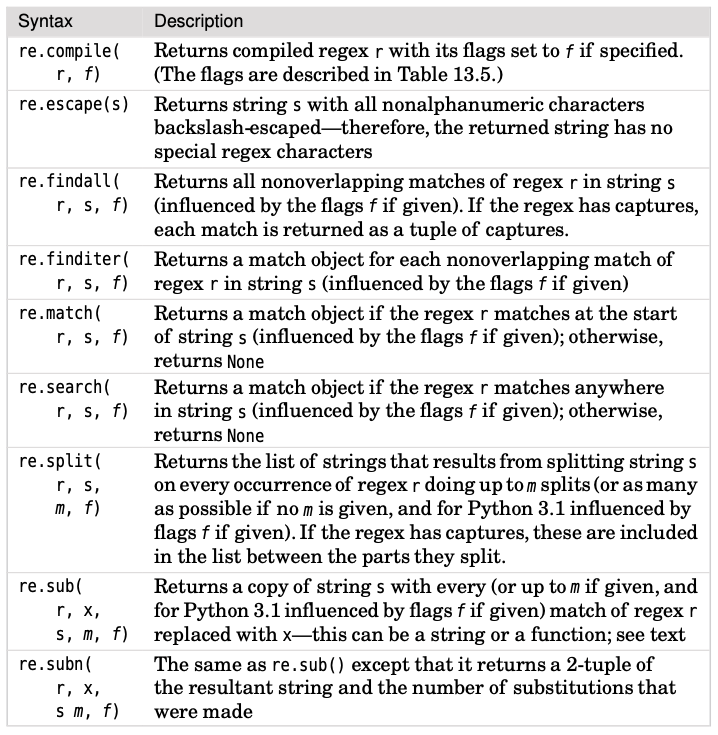
\includegraphics[width=\textwidth]{pics/regex-first-way}
  \caption{The Regular Expression Module’s Functions}
  \label{fig:regex-first-way}
\end{figure}


\begin{figure}[!ht]
  \centering
  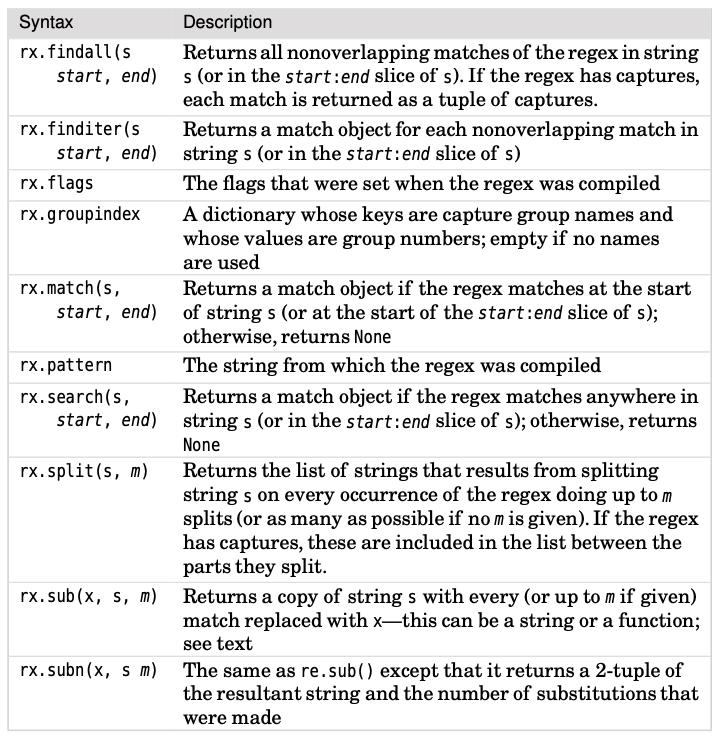
\includegraphics[width=\textwidth]{pics/regex-second-way}
  \caption{Regular Expression Object Methods}
  \label{fig:regex-second-way}
\end{figure}


\begin{figure}[!ht]
  \centering
  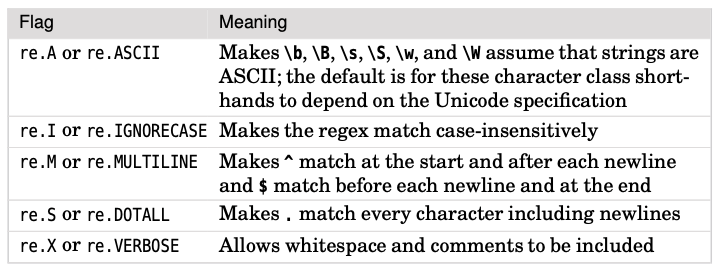
\includegraphics[width=\textwidth]{pics/regex-flag}
  \caption{The Regular Expression Module's Flags}
\end{figure}


For example (search):
\begin{lstlisting}
import re

# manner 1
text = '#C0C0AB'
match = re.search(r'#[\dA-Fa-f]{6}\b', text)

# manner 2
color_re = re.compile(r'#[\dA-Fa-f]{6}\b')
match = color_re.search(text)

# flag
match = re.search(r'#[\dA-F]{6}\b', text, re.IGNORECASE)
match = re.search(r'(?i)#[\dA-F]{6}\b', text)
\end{lstlisting}


The methods provided by match objects are listed in Figure \ref{fig:match-object-methods}
\begin{figure}[!ht]
  \centering
  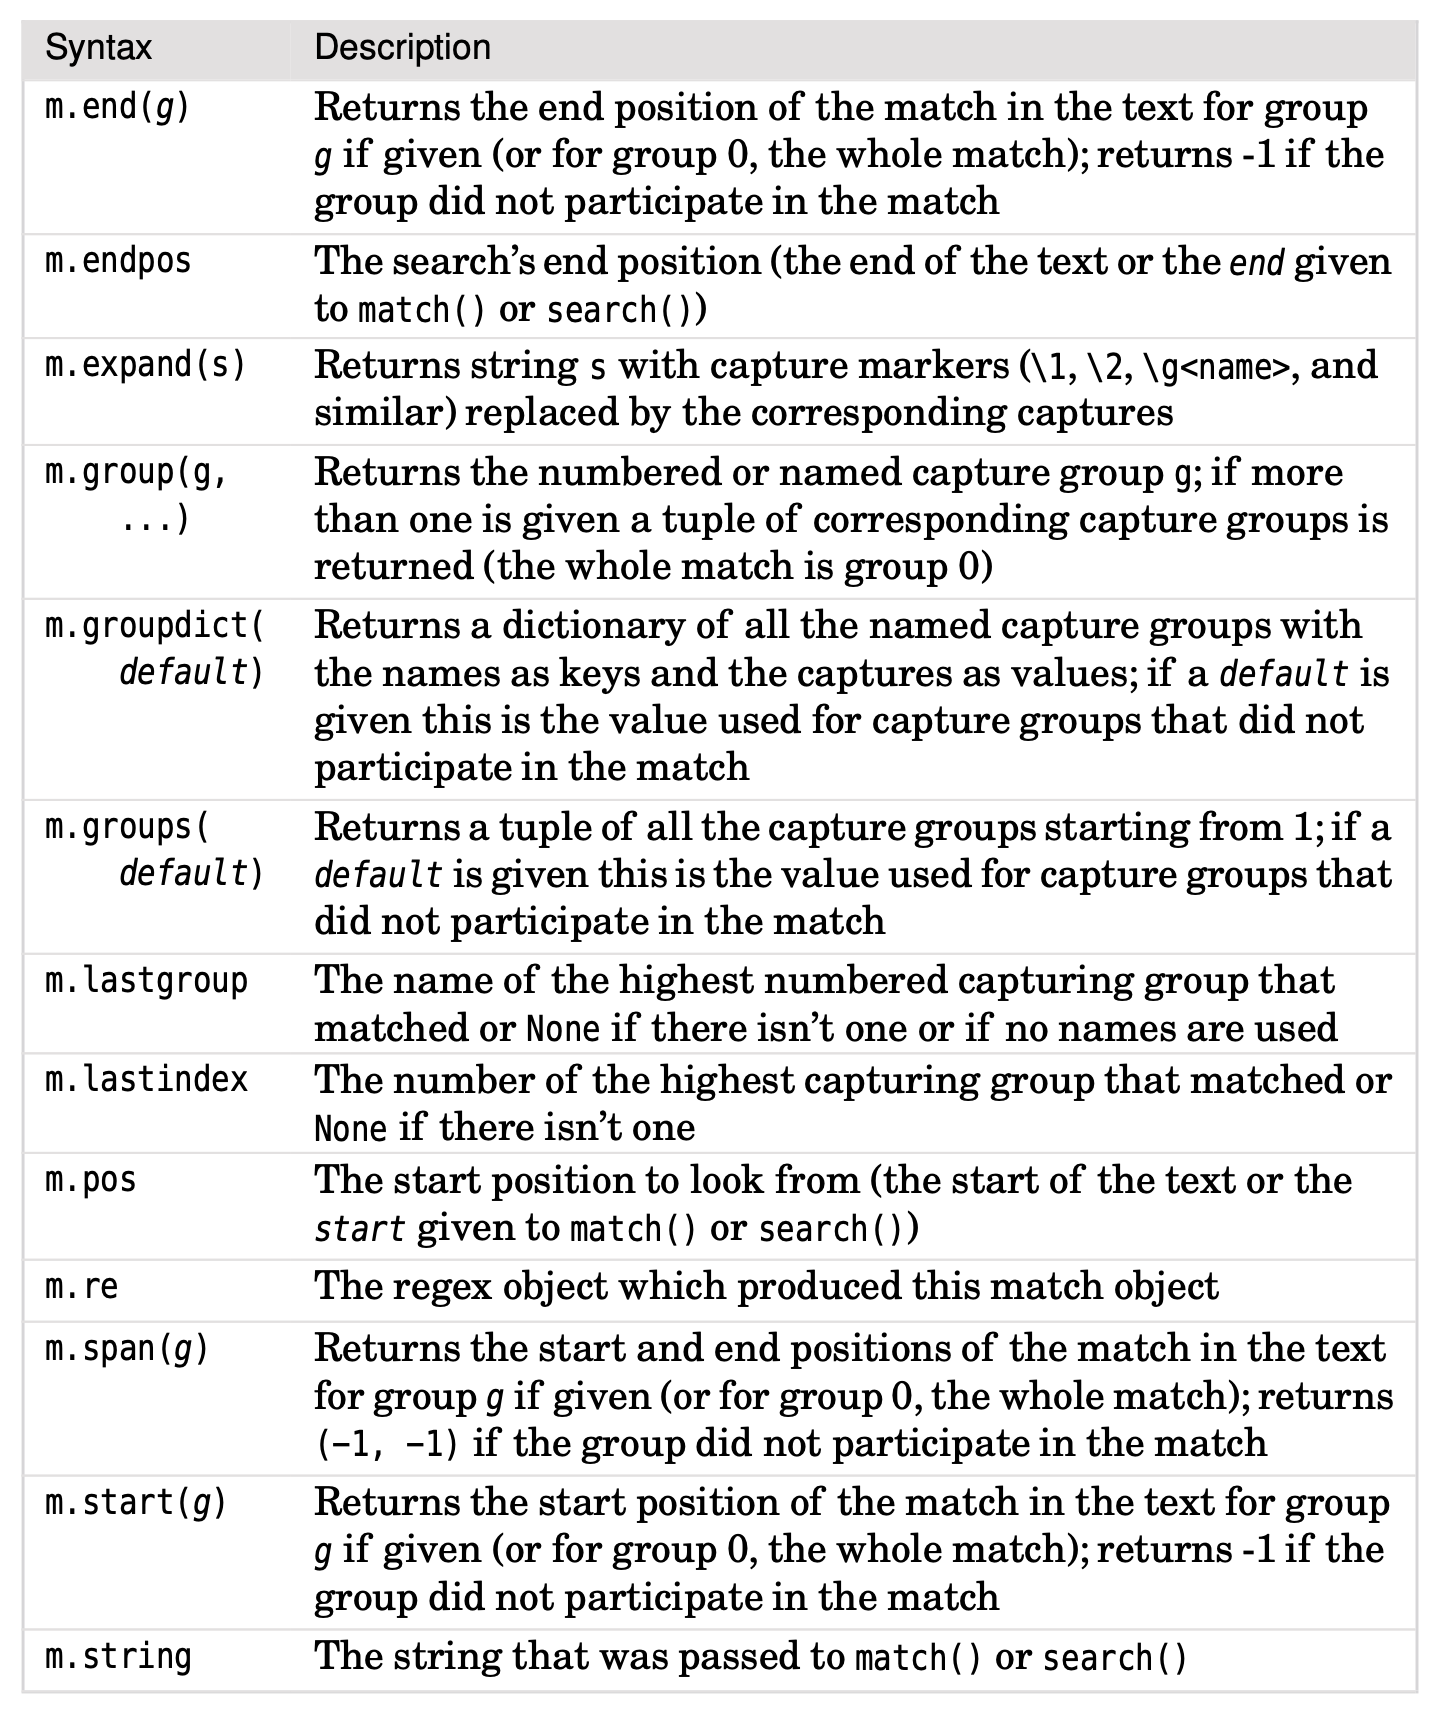
\includegraphics[width=\textwidth]{pics/match-object-methods}
  \caption{Match Object Attribute and Methods}
  \label{fig:match-object-methods}
\end{figure}

Example (check duplicate words):
\begin{lstlisting}
text = "one and and two let's say"
double_word_re = re.compile(r"\b(?P<word>\w+)\s+(?P=word)(?!\w)", re.IGNORECASE)
double_word_re = re.compile(r"\b(?P<word>\w+)\s+(?P=word)\b", re.IGNORECASE) # same to the above
for match in double_word_re.finditer(text):
    print(f'{match.group("word")} is duplicated')
# and is duplicated
\end{lstlisting}


Example (extract image filenames):
\begin{lstlisting}
text = '''
<img src="/images/stickman.gif" alt="Stickman" width="24" height="39">
<img src="https://www.w3schools.com/images/lamp.jpg" alt="Lamp" width="32" height="32">
'''
image_re_text = r'''
<img\s+                              # start of the tag
[^>]*?                               # any attributes that precede the src
src=                                 # start of the src attribute
(?:
     (?P<quote>["'])                 # opening quote
     (?P<qimage>[^\1>]+?)            # image filename
     (?P=quote)                      # closing quote matching the opening quote
|
     (?P<uimage>[^"' >]+)            # unquoted image filename
)
[^>]*?                               # any attribute that follow the src
>     
'''
image_re = re.compile(image_re_text, re.IGNORECASE | re.VERBOSE)
image_files = []
for match in image_re.finditer(text):
    image_files.append(match.group("qimage") or match.group("uimage"))
for image_file in image_files:
    print(image_file)
# /images/stickman.gif
# https://www.w3schools.com/images/lamp.jpg  
\end{lstlisting}



Example (convert html to text):
\begin{lstlisting}
def html2text(html_text):
    def char_from_entity(match):
        code = html.entities.name2codepoint.get(match.group(1), 0xFFFD)
        return chr(code)

    # (?s) math . include newline
    text = re.sub(r"(?s)<!--.*?-->", "", html_text)  # HTML comments
    text = re.sub(r"<[Pp][^>]*?>", '\n\n', text)  # opening paragraph tags
    text = re.sub(r"<[^>]*?>", '', text)  # any tag
    text = re.sub(r"&#(\d+);", lambda m: chr(int(m.group(1))), text)  # &#165; for ¥
    text = re.sub(r"&([A-Za-z]+);", char_from_entity, text)  # named entities
    text = re.sub(r"\n(?:[ \xA0\t]+\n)+", '\n', text)  # linesthat contain only whitespace
    # Replace sequences of two or more newlines with exactly two newlines
    text = re.sub(r"\n\n+", '\n\n', text.strip())
    return text  
\end{lstlisting}


Example (switch name order in fullname):
\begin{lstlisting}
import re

# from Forename Middlename1 ... MiddlenameN Surname
# to Surname,ForenameMiddlename1...MiddlenameN
names = ['Mike Ming Chyson', 'Maël Ming Li']
new_names = []
for name in names:
    # name = re.sub(r"(\w+(?:\s+\w+)*)\s+(\w+)", r"\2, \1", name)
    name = re.sub(r"(?P<forenames>\w+(?:\s+\w+)*)"
                  r"\s+(?P<surname>\w+)",
                  r"\g<surname>, \g<forenames>",
                  name)
    new_names.append(name)
for name in new_names:
    print(name)
# Chyson, Mike Ming
# Li, Maël Ming  
\end{lstlisting}


Example (detect encoding):
\begin{lstlisting}
import re

binary = b''

re_binary = r"""
# A lookbehind assertion that says that the
# match cannot be preceded by a hyphen or a word character.
(?<![-\w]) 
(?:(?:en)?coding|charset)  # encoding|coding|charset
(?:=(["'])?([-\w]+)(?(1)\1)
|:\s*([-\w]+))
""".encode('utf8')
match = re.search(re_binary, binary, re.IGNORECASE | re.VERBOSE)
encoding = match.group(match.lastindex) if match else b'utf8'
\end{lstlisting}

Example (split text based on whitespace):
\begin{lstlisting}
text = 'hello world'
re.split(r"\s+", text)
# same to
text.split()  
\end{lstlisting}

\chapter{Introduction to GUI programming}

Python has no native support for GUI (Graphical User Interface) programming, but this isn't a problem since many GUI libraries written in other languages can be used by Python programmers.
This is possible becuase many GUI libraries have Python \keyword{wrappers} or \keyword{bindings} -- these are packages and modules that are imported and used like any other Python packages and modules but which access functionality that is in non-Python libraries under the hood.


Python's standard library includes Tcl/Tk -- Tcl is an almost syntax-free scripting language and Tk is a GUI library written in Tcl and C.
Python's \verb|tkinker| module provides Python binding for the Tk GUI library.
Tk has three advantages compared with other GUI libraries:
\begin{itemize}
\item It is installed as standard with Python, so it is always available.
\item It is small.
\item It comes with IDLE.
\end{itemize}



For developing GUI programs that must run on any or all Python desktop platform, using only a standard Python installation with no additional libraries, there is just one choice: Tk.



\section{Dialog-style programs}

In most object-oriented programs, a custom class is used to represent a single main window or dialog, with most of the widgets it contains being instances of standard widgets, such as buttons or checkboxes, supplied by the library.
Like most cross-platform GUI libraries, Tk doesn't really make distinction between a window and a widget -- a window is simply a widget that has no widget parent.
Widgets that don't have a widget parent (windows) are automatically supplied with a frame and window decorations (such as a title bar and close button).
In addition to distinguishing between widgets and windows (also called top-level widgets), the parent–child relationships help ensure that widgets are deleted in the right order and that child widgets are automatically deleted when their parent is deleted.

The interface is shown in Figure \ref{fig:interest}.
\begin{figure}[!ht]
  \centering
  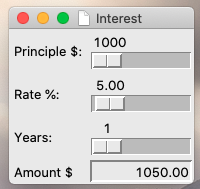
\includegraphics[width=0.8\textwidth]{pics/interest}
  \caption{The interest program}
  \label{fig:interest}
\end{figure}

The corresponding code is shown below:


\begin{lstlisting}
#!/usr/bin/env python3
"""
@project: python3
@file: interest
@author: mike
@time: 2021/2/23
 
@function:
"""
import tkinter
import os
import sys


class MainWindow(tkinter.Frame):
    def __init__(self, parent):
        super().__init__(parent)
        self.parent = parent
        # Lays out the frame using the grid layout manager
        self.grid(row=0, column=0)

        self.principal = tkinter.DoubleVar()
        self.principal.set(1000.0)
        self.rate = tkinter.DoubleVar()
        self.rate.set(5.0)
        self.years = tkinter.IntVar()
        self.amount = tkinter.StringVar()

        principal_label = tkinter.Label(self, text='Principle $:',
                                        anchor=tkinter.W,
                                        underline=0)
        principal_scale = tkinter.Scale(self, variable=self.principal,
                                        command=self.updateUi,
                                        from_=100,
                                        to=10000000,
                                        resolution=100,
                                        orient=tkinter.HORIZONTAL)
        rate_label = tkinter.Label(self, text='Rate %:',
                                   underline=0,
                                   anchor=tkinter.W)
        rate_scale = tkinter.Scale(self, variable=self.rate,
                                   command=self.updateUi,
                                   from_=1,
                                   to=100,
                                   resolution=0.25,
                                   digits=5,
                                   orient=tkinter.HORIZONTAL)
        year_label = tkinter.Label(self, text='Years:',
                                   underline=0,
                                   anchor=tkinter.W)
        year_scale = tkinter.Scale(self, variable=self.years,
                                   command=self.updateUi,
                                   from_=1,
                                   to=50,
                                   orient=tkinter.HORIZONTAL)
        amount_label = tkinter.Label(self, text='Amount $', anchor=tkinter.W)
        actual_amount_label = tkinter.Label(self, textvariable=self.amount,
                                            relief=tkinter.SUNKEN,
                                            anchor=tkinter.E)

        principal_label.grid(row=0, column=0, padx=2, pady=2, sticky=tkinter.W)
        principal_scale.grid(row=0, column=1, padx=2, pady=2, sticky=tkinter.EW)
        rate_label.grid(row=1, column=0, padx=2, pady=2, sticky=tkinter.W)
        rate_scale.grid(row=1, column=1, padx=2, pady=2, sticky=tkinter.EW)
        year_label.grid(row=2, column=0, padx=2, pady=2, sticky=tkinter.W)
        year_scale.grid(row=2, column=1, padx=2, pady=2, sticky=tkinter.EW)
        amount_label.grid(row=3, column=0, padx=2, pady=2, sticky=tkinter.W)
        actual_amount_label.grid(row=3, column=1, padx=2, pady=2, sticky=tkinter.EW)

        principal_scale.focus_set()
        self.updateUi()
        parent.bind('<Alt-p>', lambda *ignore: principal_scale.focus_set())
        parent.bind('<Alt-r>', lambda *ignore: rate_scale.focus_set())
        parent.bind('<Alt-y>', lambda *ignore: year_scale.focus_set())
        parent.bind('<Control-q>', self.quit)
        parent.bind('<Escape>', self.quit)

    def updateUi(self, *ignore):
        amount = self.principal.get() * (
                (1 + (self.rate.get() / 100.0)) ** self.years.get()
        )
        self.amount.set(f'{amount:.2f}')

    def quit(self, event=None):
        self.parent.destroy()


application = tkinter.Tk()
path = os.path.join(os.path.dirname(__file__), 'images/')
if sys.platform.startswith('win'):
    icon = path + 'interest.ico'
else:
    icon = '@' + path + 'interest.xbm'
application.iconbitmap(icon)
application.title('Interest')
window = MainWindow(application)
application.protocol('WM_DELETE_WINDOW', window.quit)
application.mainloop()
  
\end{lstlisting}




Rather than using absolute positions and sizes, widgets are laid out inside other widgets using layout managers.
The call to \verb|grid()| lays out the frame using the grid layout manager.
Every widget that is shown must be laid out, even top-level ones.


(Line 22-27)
Tk allows us to create variables that are associated with widgets.
If a variable’s value is changed programmatically, the change is reflected in its associated widget, and similarly, if the user changes the value in the widget the associated variable’s value is changed.


(Line 29-59)
This part of the initializer is where we create the widgets.
The \verb|tkinter.Label| widget is used to display read-only text to the user.
Like all widgets it is created with a parent, and then keyword arguments are used to set various other aspects of the widget’s behavior and appearance.
We have set the \verb|principalLabel|’s text appropriately, and set its anchor to \verb|tkinter.W|, which means that the label’s text is aligned west (left).
The underline parameter is used to specify which character in the label should be underlined to indicate a keyboard accelerator (e.g., Alt+P).
(A keyboard accelerator is a key sequence of the form \verb|Alt+letter| where \verb|letter| is an underlined letter and which results in the keyboard focus being switched to the widget associated with the accelerator, most commonly the widget to the right or below the label that has the accelerator.)


(Line 72-77)
We set up a few key bindings.


To give the program an icon on Windows we use an \keyword{.ico} file and pass the name of the file (with its full path) to the iconbitmap() method.
But for Unix platforms we must provide a bitmap.
Tk has several built-in bitmaps, so to distinguish one that comes from the file system we must precede its name with an \keyword{@} symbol.



\section{Main-window-style programs}

\url{https://github.com/mikechyson/python3/blob/master/c15_gui/bookmarks_tk.pyw}
\chapter{Environment}

The operating system is Ubuntu 20.04.1 LTS.

The text editor is Emacs.

The installation of Emacs is as follows:

\lstset{language=sh}
\begin{lstlisting}
  sudo apt install emacs
\end{lstlisting}

The installation of LaTex and some packages is as follows:
\begin{lstlisting}
  sudo apt install texlive-latex-base
  sudo apt install texlive-xetex
  sudo apt install texlive-full
\end{lstlisting}









\backmatter
\bibliographystyle{plainnat}
\bibliography{tex}
\end{document}
